\chapter{Wordlists, cognate sets, and test data}\label{sec:4}

The purpose of this chapter is to describe the infrastructure that was developed to arrive at the linguistic dataset used for evaluation of the new algorithms I propose in Chapters 6 and 7. The first section describes the NorthEuraLex database, which has been the major data collection project within the EVOLAEMP project, and of which the author has been the coordinator and most active contributor. Further sections describe how the orthographic realizations as extracted from dictionaries were converted into a phonetic representation, the rather complex way in which phonetic strings were aligned to yield similarity scores, and the way in which cognate sets where inferred from these scores through clustering.

\section{NorthEuraLex}\label{sec:4.1}

\subsection{The case for a new deep-coverage lexical database}
Existing large-scale lexical databases only contain data for very few concepts. While Swadesh lists of between 100 and 250 concepts exist for many languages, there has so far not been an effort to collect such lists across many language families. The singular cross-linguistic database with truly global coverage is the ASJP database \citep{asjp17}, which by now covers a list of 40 very stable concepts across more than 5,000 languages.

Typically, algorithms for more advanced subtasks such as sound correspondence extraction and automated reconstruction are tested and evaluated on data covering a single language family. The best deep-coverage databases in a uniform format are maintained by experts in the respective language families.

The only deep-coverage lexical database which covers a multitude of language families is the intercontinental dictionary series (IDS) edited by \cite{ids}. This collection of dictionaries has the advantage of consisting of expert contributions, but has not been extended for a long time, and remains at just over 329 different languages from all over the world. The disadvantages of this database are that it does not cover any larger geographical area which could be used for contact models, that there are large gaps in lexical coverage even for languages where more complete resources would be available, and that it does not include a uniform phonetic representation across all languages, tending to favor orthographic forms instead.

Faced with this landscape, the members of the EVOLAEMP project made the decision to develop a new deep-coverage database for a contiguous geographical area that can be covered by collecting data from around a hundred languages.

\subsection{Selecting the language sample}
The linguistic interests of the author and the existence of previously collected data suggested Northern Eurasia as a good linguistic area to cover comprehensively. Within this area, the idea was to focus on a language family about which much is known already, in order to be able to evaluate the results of automated method against existing knowledge. Moreover, the language sample should be small enough to make comprehensive coverage within the time frame of the project feasible, while at the same time covering at least one family and all of its relevant contact languages in neighboring families, in order to have good test cases for models of lexical influence.

The feasibility constraint initially excluded Indo-European\il{Indo-European languages} with its hundreds of languages as the central focus, and most Siberian languages were not ideal due to the sparseness of established etymological knowledge. As a middle ground, the Uralic language family quickly appeared as an ideal test case, because it features comprehensive research which goes back in time at least as far as Indo-European linguistics, yet is manageable in size at about 30 to 40 languages, depending on how dialects are counted. The core of the language sample for NorthEuraLex is therefore formed by a high coverage of \ili{Uralic languages}. The 26 Uralic languages for which data were collected represent essentially all the Uralic languages for which published dictionaries or other comprehensive lexical resources are available, making it possible to retrieve almost-complete large word lists.

To extend this core of 26 languages in the direction of the desired sample size, we added to the sample all the languages which are known to have been in intensive contact with Uralic languages during their history. For the western branches of Uralic, these include Germanic\il{Germanic languages} (German, Swedish, Norwegian) and Baltic (Latvian and Lithuanian) languages. Contact with \ili{Slavic languages} (especially Russian) has of course been particularly intense across all the minority languages of Russia, but this also applies to the Saami and Finnic languages in the West. There are some very old loans from Proto-Iranian (including the words for `hammer', `a hundred') into Proto-Uralic, leading us to include \ili{Ossetian} as the closest living descendant of the Scythian languages. The central Uralic languages have been in intensive contact with \ili{Turkic languages} (Chuvash, Tatar, and Bashkir), whereas the \ili{Samoyedic languages} to the east had some contacts with \ili{Siberian Turkic languages} as well as \ili{Yeniseian languages}. The interaction of \ili{Hungarian} with many of its neighbors adds a substantial number of additional languages (Slovak, Croatian, Romanian, and Turkish) to the set. The inclusion of these languages provides many interesting example cases for models of lexical contact.

To further expand the language sample, we decided to more extensively sample all the language families touched upon, by including at least one language from each surviving branch of Indo-European and Turkic. Due to the familiarity of many project members with several Indo-European languages, the Indo-European sample was further extended by many national languages of Europe. In order to have some data that can be used to develop statistical tests of long-distance connections, and to enlarge the area of coverage eastwards, we decided to also collect data from all the well-documented Paleosiberian languages, and the other branches of the contested Altaic language family besides Turkic, i.e.\ Mongolian and Tungusic, as well as the even more contested Korean and Japanese.

To further increase variation in the data, and to close the gaps between linguistic areas we already covered, we further included the four major \ili{Dravidian languages} as well as a substantial sample of the indigenous languages of the Caucasus (all three families). Finally, we also added well-documented isolates such as \ili{Basque} and \ili{Burushaski}, as well as \ili{Arabic}, \ili{Hebrew}, and \ili{Mandarin Chinese}, languages of adjacent families with strong influences on many languages in the sample. These languages had to be added in order to be able to model e.g. the common Arabic influence on many languages of the Middle East as well as the Caucasus, which would otherwise appear closely related due to the many loans from Arabic.

Appendix A contains the resulting list of languages in the current version of NorthEuraLex,
along with their genetic affiliations according to Glottolog \citep{glottolog}.

\subsection{Selecting and defining the concepts}
With the language sample in place, the next question for the design of a lexical database is which concepts to cover. The only long concept list that currently seems to be in use for massively cross-linguistic lexical databases is the IDS list, which is based on \cite{buck1949}, who uses a rather subjectively compiled list geared towards \ili{Indo-European languages}. Using the results of the WOLD project, \cite{tadmor2009} distills a more empirically motivated ranking of the 100 concepts least susceptible to borrowing, the Leipzig-Jakarta list.

In order to define a list of 1,000 basic concepts on a more empirical basis, we decided to use existing digitalized dictionary data for 12 languages in order to develop computational criteria that capture the notion of basicness, and to use these criteria in order to rank a large list of concepts as to their appropriateness of inclusion into Swadesh-type lists (``swadeshness''). In \cite{dellert_buch_2015}, we ranked about 6,000 concepts defined by sets of German glosses (for disambiguation) by a linear combination of two measures. The first measure quantifies basicness in terms of average realization length, which is based on phoneme sequence length, but uses the information weighting which will be presented in \sectref{sec:4.3.1} to correct for language-specific effects of phoneme inventory size as well as for the differences between stems and dictionary forms. The second measure is the correlation of realization distances and overall language distances for a sample of language pairs drawn with equal probability
from language pairs of all distances. Individual form distances were inferred by a variant of IWSA as presented in \sectref{sec:4.3.3}, and the language distances were aggregated from the form distances for 50 basic concepts by the dER measure \citep{jaeger2013}. This local-global distance correlation is high (in the vicinity of 0.9) for concepts where the form distances mirrored the overall language distances very well (e.g. \textsc{bone}), much lower for concepts which disturb the fit to the phylogeny due to frequent loans (e.g. \textsc{bread}), and near zero for words which were borrowed from a single language across the globe (e.g. \textsc{computer}). The combined measure thus favors concepts which are associated with short words in many languages, have similar realizations in related languages, and dissimilar realizations in unrelated languages. The 1,000 best concepts according to this initial ranking of 6,000 rather coarsely defined concepts formed our starting point which we then refined into the final concept list for NorthEuraLex.

Starting with the initial list, we began working on the languages for which lexical resources are most sparse, and to which the concept list was therefore supposed to be adapted with the goal of ensuring near-complete coverage even for smaller minority languages. For this task, I systematically extracted the Russian glosses from a series of Soviet school dictionaries that contain about 4,000 entries in both directions, which were designed with the needs of native-language school education in mind. These dictionaries, such as \cite{menovshchikov1988} for \ili{Siberian Yupik} and \cite{volodin1989} for \ili{Itelmen}, are sometimes the only published lexical resource for the languages in question. Beyond a rather small core vocabulary, these dictionaries often do not cover every concept that a historical linguist might be interested in (such as \textsc{louse} or \textsc{mother\_in\_law}), but much basic vocabulary that is essential to the native cultures such as different types of sleighs and tents, or names of birds
and fish. Intersecting these specialized lists, a pan-Siberian list of region-specific, but very well-represented concepts such as \textsc{elk} and \textsc{eagle} emerged, which were used to replace some of the harder-to-find items from the automatically extracted concept list. After the data were collected, these concepts also turned out to rank rather highly in our ``swadeshness'' measure, because their realizations are short and phylogenetically informative across the entire region.

The resulting list of 1,016 concepts can be separated into four main categories. The list of nominal concepts (concepts which are predominantly expressed by nouns across the sample) contains 480 items, including typical Swadesh concepts such as 48 parts of the body, but also 34 North Eurasian animal names, and the words for months and days of the week. The next largest category of 340 items is subsumed as verbal concepts, because they are words describing actions which are cross-linguistically most frequently expressed by verbs, with a few exceptions where the best equivalents are verbal suffixes. Typologically most difficult to define is the list of 102 adjectival concepts, typically properties of objects, the words for which behave similarly to nouns in some, and similarly to verbs in other languages. Since we will typically only be interested in stems, we decided to collect the equivalent lexical items independently of their category in each target language. Finally, the list features 94 concepts which
typically are covered by words from closed classes. These include personal pronouns, some basic adverbs (e.g.\ \textsc{today} and \textsc{tomorrow}), a few spatial adpositions (e.g.\ \textsc{behind} and \textsc{through}), cardinal numbers, as well as a few conjunctions.

Many concepts needed to be disambiguated by additional annotations. For instance, many languages (such as \ili{Spanish}) have different basic words for front teeth and back teeth, and our annotation for the concept \textsc{tooth} says that the word for the human incisor will always be listed first. Also the concept \textsc{uncle} is represented in many languages by at least two different words with the meanings \textsc{brother\_of\_father} and \textsc{brother\_of\_mother}, and our annotations define the first one as the default choice in this situation. To disambiguate verbal meanings, we often rely on prototypical arguments, as in \textsc{blow [wind]}, \textsc{melt [ice]}, and \textsc{knock [on wall]}. Sometimes, we also add paraphrases, as for \textsc{smoke}, which we annotate by \textsc{[emit smoke]} to distinguish it from `smoking cigarettes'.

Within the project, we produced translations of the concept list and the annotations into the other two most important gloss languages, English and Russian. While internally, \ili{German} is the primary language of the database, for ease of exposition I will only quote the English translations in this book. The full English version of the concept list with the annotations can be found in Appendix A.

\subsection{The data collection process}
Some details of the data collection process are described in \cite{dellert2015a}. In the two years since, data collection has progressed roughly in the same manner described there for the Uralic part of the dataset. A summary of the procedure is repeated here, with some changes that occurred during the following two years.

For the languages where several lexical resources were available, we did not base our decision on the immediate accessibility of the respective gloss language, but on a preference for work describing the standard language. For many \ili{Uralic languages}, this meant we did not rely on scientific dictionaries in German or English, but on Russian dictionaries of the standard languages. When starting to work with a dictionary for one of the target languages, it was frequently necessary as a first step to translate the concept list into the gloss language of that dictionary. For languages other than English or Russian, we did not produce independent versions of the concept list by translating the annotations, but relied on the previously collected data for the gloss language instead. This was our strategy for the following gloss languages: \ili{Norwegian} (for the \ili{Western Saami languages}), \ili{Swedish} (for some information on \ili{Southern Saami}), \ili{Finnish} (for \ili{Inari Saami} and \ili{Skolt Saami}), \ili{Estonian} and \ili{Latvian} (for \ili{Livonian}), \ili{Hungarian} (for some information on Northern \ili{Mansi} and \ili{Nganasan}), \ili{French} (for \ili{Breton}), \ili{Japanese} (for some information on \ili{Ainu}), and \ili{Chinese} (for some information on \ili{Manchu}).

Given the list of relevant lemmas in the gloss language, the first step of the data retrieval process consisted in looking up all the lemmas in the gloss-to-target language dictionary, and keeping track of possible disambiguating information in a standardized format. Entries were usually typed in the original standardized orthographies to ensure ease of automated retrieval, and compatibility across different resources. For the second step, the lookup list produced in this way was reverted, and alphabetically sorted in the target language. All target lemmas were then looked up in the target-to-gloss language dictionary, in order to retrieve as much disambiguating information as possible on all the possibly relevant target lexemes. Frequently, information from example sentences found in the dictionary was included in annotations to the gloss-language translations in a standardized way.

The final stage consiste in defining a lookup filter which stores the selection decisions concerning the best equivalent of each concept in the target language. The decisions were mainly based on automatically generated PDF summaries of the lookup information in both directions (often about 500 pages of information for the 1,016 concepts in our final list). Sometimes, this process was supported by semi-automated translation of the gloss language into German. Often, we also relied on a variety of additional resources such as grammars, introductory textbooks, the Wikipedia in various languages, example sentences from the collaborative database Tatoeba \citep{tatoeba}, and Google phrase searches to clarify the contexts in which certain words are used.

\subsection{Difficulties and future development}
The main complication during data collection was that many of the selection choices were difficult to make based on the little information that is sometimes included in dictionaries, which are often the only resources available for smaller minority languages. While the preference for school dictionaries somewhat alleviated the situation, as only the most natural or basic translation for each gloss language lemma is given, more precise information especially on verbal concepts was found to be very difficult to obtain.

For these reasons, the version of NorthEuraLex which was used in the work described here is a first nearly complete version which, however, unavoidably still contains many errors. To further improve on data quality, much expert feedback will be necessary. Due to the design decision not to try to get word lists directly from experts, it was possible to get initial coverage of a large geographic region within little more than two years. Also, the uniform data collection process with extensive protocols and information tracking makes it feasible to continually revise and improve decisions, which would be much harder to organize if a different person were responsible for each language.

The data for the Uralic languages have been available for other researchers since early 2015 \citep{dellert2015a}. Larger parts of the data were also used in and are distributed together with a paper \citep{dellert2016a} that presents an early prototype of the lexical flow inference algorithm I am developing and evaluating in this book. As additional parts of the NorthEuraLex database reached pre-final stages, they were first used within the project to evaluate new methods of sound correspondence detection, linguistically motivated alignment, and cognate detection, and version 0.9 was released in June 2017 for download via a web interface which also provides capabilities for exploring the dataset in a browser.\footnote{\url{www.northeuralex.org}} The data which my work in this book builds on have thus been released under a CC-BY license which allows other researchers to build on and expand on these data, and due to its coverage of many language families central to historical linguistics, it is hoped that NorthEuraLex will become one of the more widely used cross-linguistic lexical databases.

Supported by an intramural research fund at the University of Tübingen, as well as by an MWK-RiSC grant from the Research Seed Capital program of the state of Baden-Württemberg, I was able to start the second phase of NorthEura\-Lex in October 2018. During the coming two years, this funding will make it possible to expand the database by many additional languages, and to add an etymological annotation layer to some core families based on aggregating information from various etymological dictionaries. The additional languages planned for this round of expansion include 27 ancient and historical languages, as well as 62 additional living languages, from the families already covered by version 0.9. The focus among ancient and historical languages will be on Indo-European, with ten ancient languages (such as \ili{Gothic}, \ili{Sanskrit}, \ili{Hittite}, and \ili{Tocharian}) and ten older variants of modern languages (e.g. \ili{Old English} and \ili{Classical Armenian}). For the living languages, expansion focuses on Central Asia with 17 additional Turkic\il{Turkic languages}, five Mongolic\il{Mongolic languages}, and seven \ili{Tungusic languages}, the Caucasus with ten further languages from the three indigenous families, as well as increasing the density of coverage in Europe by 18 further living \ili{Indo-European languages} (e.g. \ili{West Frisian}, \ili{Galician}, and Upper \ili{Sorbian}). Altogether, these expansions are planned to increase the number of languages in NorthEuraLex from 107 to 196.

To improve the quality of the existing NorthEuraLex data beyond the state achievable by extraction work from dictionaries, it will be vital to get into contact with experts for the individual languages. This type of work is planned to be carried out much more systematically after the current stage of expansion. Initial contacts with expert communities have already been formed, and in addition, a database of native speaker contacts is maintained by the author. In initial experiments with native speakers of \ili{Hungarian}, \ili{Italian}, \ili{Ukrainian}, and \ili{Japanese}, the ratio of clearly wrong selection entries which had to be revised based on their feedback varied between 1.3\% and 3.9\%.

Regarding less well-documented minority languages, we have been able to get at least an impression of data quality by getting feedback from a native speaker of \ili{Udmurt}, with whom the reviewing process for the entire concept list took just under seven hours. This experiment resulted in improvements to just under 9\% of selection decisions in the initial non-expert version. Udmurt was a particularly difficult case due to the outdatedness of the available dictionaries, and a lack of example sentences in them. I would therefore expect the error rates for other smaller languages to be somewhere between the range observed for the well-documented languages, and the figure determined for Udmurt.

Some clear patterns emerged when comparing the errors made for the different languages. Problems very much tend to cluster around some concepts which turned out to be particulary difficult to look up in dictionaries, such as the difference between hitting on a table and hitting a person, or the differences between paws and claws. Even for the data which we will not manage to check with native speakers or experts, we will be able to flag the data for certain concepts as more or less reliable, allowing users of the database to reduce the expected error rate by excluding the data for such concepts when using our database. I estimate that in this way, error rates of under 2\% for a reduced list of 900 concepts will be possible for users who need better data quality for their applications.

\section{Transforming and encoding into IPA}\label{sec:4.2}
With the collected lemmas for each concept and the selection filters, we now have lists of parallel orthographic forms for more than 1,000 concepts across 107 languages. To make these strings of symbols comparable, it is necessary to convert all the data into some uniform phonetic representation. For this purpose, we made the decision to semi-automatically convert all the data into the relevant subset of the International Phonetic Alphabet (IPA). The following sections represent the reasons for as well as the advantages and difficulties associated with this design decision, also discussing possible alternative options. The technical details behind the conversion process cannot be explained for every language, but a general overview of the system architecture and its capabilities is given. Also, I describe and motivate our approach to segmenting the resulting IPA strings in such a way that the gappy bigram models as well as pointwise mutual information models of sound correspondences that will be used later on do not become too sparse.

\subsection{Encoding cross-linguistic sound sequence data}
Several encoding schemes for cross-linguistic lexicostatistical work have been developed before. One of the earliest and still rather popular options was introduced by Aharon Dolgopolsky in his seminal work \citep{dolgopolsky1964} on possible deep ancestral relationships among the languages of Northern Eurasia. The \isi{Dolgopolsky encoding} only distinguishes eleven fundamental sound classes. Vowels are not differentiated at all (class \texttt{V}), and consonants are almost exclusively differentiated by place of articulation, where dental and alveolar affricates are grouped together with velar obstruents (class \texttt{K}), and all sibilants fall in the same class \texttt{S}, as do all liquids (class \texttt{R}). Nasals are differentiated into labial \texttt{M} and other nasals \texttt{N}. The final two classes group together palatal approximants \texttt{J} and voiced labial fricatives \texttt{W}. While this encoding scheme is plausible for the purpose of detecting possible deep signals in order to assess the support for macrofamilies, it is much too coarse for computational tasks that are closer to mainstream historical linguists. For instance, virtually all instances of sound change take place within the same Dolgopolsky class. The encoding scheme is not designed for capturing sound shifts, but for abstracting over them.

A slightly more fine-grained encoding scheme is the SCA sound-class model\is{SCI encoding} used by the LingPy toolkit \citep{list_forkel_2016}. The version described in \cite{list2012sca} combines 28 sound classes with prosody classes, which are used to keep apart sound correspondences in different prosodic positions. Unlike the Dolgopolsky model, SCA distinguishes six vowel classes, and it adds five additional classes to encode consonants. The remaining seven sound classes are reserved for encoding different tones, indicating that this encoding scheme is especially suited for encoding data from tonal languages at a high level of detail. On the other hand, like in the Dolgopolsky model, there is only a single class for the sibilants, and no voicing contrast is modeled for any phoneme pair. Vowel features beyond tone, like length or nasalization, are not distinguished either, which makes the model very uneven in its ability to represent data from different language families.

Among widespread phonetic encoding schemes, the next in order of granularity is the \isi{ASJP encoding}, which was developed as part of the Automated Similarity Judgment Program (ASJP), and provides the unified encoding for the ASJP database which was already discussed in \chapref{sec:2}. On the most elementary level, this encoding distinguishes 41 sound classes, and uses both uppercase and lowercase characters of the Latin alphabet as well as digits to represent them as symbols. An extended version based on diacritics is also defined, but already the basic version can express many relevant distinctions. Still, some distinctions seem slightly idiosyncratic (cf. the introduction of a special class for the dental nasal, which is only phonemically distinct from the alveolar nasal in very few languages of the world), whereas other highly relevant distinctions are not made (e.g.\ between retroflex and apical consonants). Still, the ASJP encoding has the advantage of already being used by the largest massively cross-linguistic lexicostatistical database in existence, and has proven its usability for asking and answering many interesting questions about phonetic universals. At the same time, the ASJP encoding is seen by most linguists as still abstracting away over too much possibly relevant detail, discarding information that might have been valuable.

With the availability of larger lexical databases of higher quality, the general trend in the field has been to move towards full IPA. The technical difficulties in handling IPA in not fully standardized Unicode encoding can be circumvented via the \isi{X-SAMPA encoding} by \cite{wells1995}, and since all existing sound-class models can easily be defined in terms of equivalence classes of IPA symbols, it is trivial to project IPA-encoded data into more coarse-grained representations as desired. This is the approach exemplified by LingPy. If given input data in IPA, the system will estimate sound correspondences and compute alignments on the level of SCA classes or any user-specified model, and then map the output alignment back to the IPA input segments. This indirect approach helps to avoid sparsity problems when inferring sound correspondences from short word lists, but risks missing some correspondences, e.g.\ if [t] and [d] correspond to different sounds in a related language, as is the case for the language pair English and German. In contrast, the system I will describe in the following sections works on an only slightly reduced version of IPA internally. This makes it unnecessary to distinguish internal phonetic representations from display and input formats, but comes at the cost of higher minimum requirements in terms of the number of cognate pairs if the goal is to infer good correspondences. However phonetic encoding is handled internally, IPA support has the advantage of allowing the user to work at the customary level of detail, and in a well-established representation format. Therefore, fully fledged IPA input and output support will lead to much higher acceptance in the wider linguistic community.

\subsection{Implementing orthography-to-IPA transducers}
Faced with the problem of transcribing thousands of lexemes from dozens of unfamiliar languages into IPA, it seemed prudent to not perform the IPA conversion manually, but try to automatize it as much as possible in order to be able to revise misconceptions later on, without having to manually retranscribe thousands of lexemes after each incremental change.

While the majority of modern orthographies feature a reasonably straightforward grapheme-to-phoneme correspondence, there are some historically grown orthographies, especially of Western European languages, which make the task of automated transcription into IPA virtually impossible. This especially applies to \ili{English}, \ili{Danish}, \ili{Irish}, and to a certain extent \ili{French}. In these languages, phonology has changed considerably since the time their orthographies developed, and there have not been many reforms to reflect these changes. For all other languages (especially most Eastern European national languages, for which the current written standards materialized only in the nineteenth century), it proved feasible to derive an acceptable approximation to the standard pronunciation from the orthography, or a standard transcription.

Still, in most languages there are some phenomena which require much familiarity with the language to transcribe correctly. For instance, while the pronunciation of Standard \ili{German} word forms is largely predictable from the orthography, there are many recent loans, especially from \ili{French} and \ili{English}, which are pronounced rather closely to the original forms. A second issue with German and other \ili{Germanic languages} is that certain frequently recurring morphemes (such as verbal prefixes) deviate from the usual rules of pronunciation. For instance, the German verbal prefix \textit{ver-} is always syllabified separately, and the \textit{r} never becomes the onset of the next syllable. For instance, the correct pronunciation of \textit{verachten} `to despise' is [fɛɐˈʔaχtn], not [fɛˈʀaχtn]. But to teach an automated system to distinguish this case from, for instance, the pronunciation [veˈʀanda] of \textit{Veranda} is a very complex task, which our current version of automated conversion from German orthography to IPA manages only imperfectly. To make it possible to still get correct output whenever we notice such errors in the IPA transcriptions for the NorthEuraLex data, our data format allows to override automated conversion by explicitly specifiying the correct IPA for any lexeme. For IPA processing, we internally use the X-SAMPA encoding, which is then converted to the Unicode characters for further processing and display.

Even for languages which have a recent and standardized orthography, automated conversion can be challenging. This especially applies to languages where some relevant phonemic distinctions are not written in the usual orthography, because there is no ambiguity for a speaker of the language. As a case in point, consider the non-distinctiveness of the phonemes [eː] and [æː] in \ili{Latvian}, both of which are written \textit{\={e}}. This type of problem can even affect new orthographies recently designed by linguists for previously unwritten languages. To maintain some amount of consistency with the orthography of the state language, there is a tendency to incompletely represent some aspects of the phonologies of minority languages. For instance, Cyrillic-based orthographies routinely follow the \ili{Russian} model of encoding palatalization by two separate series of palatalizing and non-palatalizing vowels. At the same time, features irrelevant to Russian such as vowel length and certain distinctions in vowel quality are often not represented. While relying on the grapheme inventory of Russian as much as possible might help the practical usage of the new orthographies by native speakers, it detracts from the value of official dictionaries and written sources to the linguist. Still, instead of relying on the older, phonologically often very precise transcribed dictionaries, in the interest of cross-source comparability and accessibility for possible corrections by native speakers, we opted to operate on the official orthographies in all but a few cases (\ili{Ainu}, \ili{Burushaski}), enhancing the lexical data with transcriptions where necessary (\ili{Persian}, \ili{Pashto}, \ili{Korean}, \ili{Japanese}, \ili{Chinese}).

Another challenge in designing orthography-to-IPA transducers is the necessity to abstract over dialectal distinctions, often maintaining the fiction of a single ``received pronunciation'' which then represents the entire language. If IPA transcriptions are included in a good dictionary, they are always abstractions tuned to some picture of the ideal standard language, sometimes consciously avoiding to over-commit to a specific pronunciation. For instance, both the English and German r-sound are routinely represented as [r] in dictionaries, although in reality, this realization is very uncommon in both languages. The symbol [r] merely abstracts away from dialectal variation within \ili{English} (usually between [ɾ] and [ɻ]) and \ili{German} (usually between [ʁ] and [ʀ]). In reality, historical linguists quite frequently take dialectal variation into account when reconstructing sound changes. Still, in the absence of comprehensive dialectal data, it seemed most feasible to take the phonological descriptions in introductory literature about the various languages at face value, and to implement simple transducers as first approximations, which can then be further improved based on native speaker feedback, more specialized literature, or analyzing recorded speech.

To obtain a preliminary solution in an acceptable timeframe, we relied on a very simple transducer formalism for the first experiments on a smaller number of languages. This architecture subsequently proved flexible enough to allow other project members to implement reasonably well-performing transducers for all of the NorthEuraLex languages.

Our transducer formalism essentially consists of ordered lists of replacement rules of the general form $\alpha\beta\gamma \rightarrow \alpha\beta'\gamma$. Each transducer file contains a list of such rules which defines a single pass through the string, where the rules are tried in the order they are given. Given a situation $\alpha \bullet \beta\gamma\delta$ during the traversal, we deterministically only apply the first rule in the order which matches a prefix of the pattern $\beta\gamma\delta$. This means that if a rule $\beta \rightarrow \beta'$ comes before the rule $\beta\gamma \rightarrow \beta^*\gamma$ in the order, the latter rule will never be applied, because the first one is deterministically chosen first. Crucially, $\alpha$ and $\beta$ are not contexts in the classical sense, because they are processed and merely copied over during the rule application, leaving the string traversal in the position $\alpha\beta\gamma\delta \bullet $, i.e.\ after the entire pattern.

Using several passes defined in separate transducer files, even this simple formalism proved sufficient and quite usable for the task at hand. The only additional capacity we introduced for convenience was the possibility to define symbol classes in order to express multiple rules concisely. For instance, to enforce a typologically very common change such as [s] $\rightarrow$ [z] between vowels, it is possible to define a symbol class [\textit{vow}] and then write rules like [\textit{vow}]s[\textit{vow}] $\rightarrow$ [.]z[.], where [.] is a notation for copying the corresponding class on the left-hand side over to the right-hand side. This abstraction over simple replacement rules was the only additional feature we found necessary.

The simple nature of the formalism made a very naive prototype implementation using Java string operations performant enough to perform the entire work described in this book. Recently, Thora Daneyko has written a compiler which turns cascades of transducer files into finite-state transducers compatible with the HFST toolkit \citep{linden_ea_2011}. This promises to lead to better performance especially on longer strings, and will be a lot more accessible to other researchers who might want to use our transducers as well. A release of the HFST versions of our orthography-to-IPA converters is planned to accompany the next major version of NorthEuraLex.

\subsection{Tokenizing into reduced IPA}
Given IPA representations of all the NorthEuraLex data, the next step in my pipeline computes string distances for cognate detection. Many considerations come into play in this part of the architecture, mostly revolving around inference of a good general phoneme distance matrix and the estimation of language pair-specific sound correspondences to adapt this general distance matrix in every concrete case.

Any model which attempts to estimate segment similarity will quickly run into problems if too many parameters are to be estimated from too little data. For many language pairs where we would like to estimate correspondences (e.g.\ members of the same family), we often need to get by on little more than a hundred cognate pairs. \cite{list2012} has tackled this problem by internally reducing IPA (which his LingPy system accepts as input) to the 28 SCA equivalence classes, over which it is easy to estimate sound correspondences even based on only 100 or 200 cognate pairs.

If our goal is to derive full IPA correspondences based on the same amount of data, we quickly run into problems. For estimating sound correspondences, it turned out necessary to reduce the number of IPA segments a little. While coarticulation and other often combinable diacritics carry the number of theoretically valid IPA segments well into the thousands, there is a core of relevant segments which are encoded by a single symbol in IPA, and which can be used as a guideline to wriggle the number of IPA segments we need to consider down to a much more manageable 120. To get a sense of what would be needed to represent all languages of the world equally well, \cite{ladefoged_maddieson_1996} estimate that more than 200 vowels and 600 consonants are actually in use.

The key decision to keep things manageable was to only use IPA symbols which actually occur in the NorthEuraLex data, which excluded click sounds and some further very infrequent types of consonants. However, due to the presence of languages both with one of the richest consonant inventories (\ili{Abkhaz}) and the highest number of vowels (\ili{French}) within the sample, this measure alone is not enough to reduce the number of symbols below around 300. This very rich inventory includes many ejectives, large numbers of diphthongs and nasal vowels, and a full array of palatalized and labialized stops, plus a few pharyngealized ones (from \ili{Arabic}).

As a solution to this combinatorial problem, I decided to treat coarticulatory features such as labialization and nasalization as separate segments following the base phoneme. Apart from the obvious benefit that this brings down the number of symbols into the feasible range, this decision can also be justified from a linguistic perspective. Frequently, nasal vowels correspond to subsequent nasal consonants in cognates, because the nasalization of vowels before nasals is a quite freqent phenomenon (cf. \ili{Italian} \textit{anno} [anːo] and \ili{French} \textit{an} [ɑ̃] `year'). In an analogous way (though to a lesser degree), high front vowels are associated with palatalization, and rounded vowels with labialization. Also, support for the most frequently occurring affricates was added, at the cost of not representing any other double articulations.

The resulting list of 107 IPA segments is given in the following table, together with their phonological definition and the closest neighbors according to the global segment distance matrix whose inference will be described in the following section. Upon inspection, the reader will see that the list of segments is quite expressive, and can represent many historically relevant distinctions with ease.

My architecture includes code for tokenizing arbitrary IPA strings into these segments, which are internally handed as Unicode strings. During tokenization, the length symbol is replaced by a repetition of the preceding segment, because support for long vowels and diphthongs would again have increased the number of segments beyond the feasible range, and many sound changes between diphthongs and vowels can easily be described in a two-segment model. Also, it is vital for the implementation of various algorithms that the full phonetic features of each segment be retrievable from the segment in isolation.

\newpage \footnotesize
\begin{center}
\begin{tabular}{lll}
\hline
\_ & internal word boundary & ɑ\\
- & gap symbol (models deletion and insertion) & ˀ\ ʔ\ ˠ\ ʼ\ ˤ\ ʕ\ \color{gray}ʰ\ ʐ\ ʲ\ ɤ\ ʜ\\
m & bilabial nasal & \ ̃\\
ɱ & labiodental nasal & \ ̃\ \color{gray}n\\
n & alveolar or dental nasal & ɲ\ \ ̃\ ɳ\ ŋ\ ɱ\\
ɳ & retroflex nasal & n\\
ɲ & palatal nasal & n\\
ŋ & velar nasal & \ ̃\ \color{gray}n\ ɡ\\
p & voiceless bilabial stop & p͡f\ \color{gray}b\ β\\
b & voiced bilabial stop & β\ \color{gray}p\ w\ ʋ\\
t & voiceless alveolar or dental stop & ʈ\ c\ θ\ ð\ \color{gray}d\ t͡ɕ\ t͡s\\
d & voiced alveolar or dental stop & ɟ\ ð\ ɖ\ θ\ \color{gray}t\\
ʈ & voiceless retroflex stop & ɖ\ t\\
ɖ & voiced retroflex stop & ʈ\ d\ \color{gray}ɻ\\
c & voiceless palatal stop & t͡ɕ\ t͡ʃ\ t\ ʃ\ \color{gray}k\ t͡s\ ç\ t͡ʂ\\
ɟ & voiced palatal stop & d\ \color{gray}ɡ\ d͡ʒ\ j\ -\\
k & voiceless velar stop & c͡ç\ ç\ q\ ɢ\ \color{gray}x\ ɡ\ χ\\
ɡ & voiced velar stop & ɣ\ ɦ\ ɢ\ ʕ\ ɟ͡ʝ\ ç\ d͡z\ h\ \color{gray}ʁ\ ɟ\ k\ ŋ\ ħ\\
q & voiceless uvular stop & q͡χ\ χ\ ɣ\ ɢ\ x\ k\ ʁ\\
ɢ & voiced uvular stop & ħ\ ɡ\ q\ k\ x\\
ʔ & glottal stop & ʕ\ ʲ\ -\ \color{gray}i\ ɒ\\
t͡s & voiceless alveolar sibilant affricate & t͡ʃ\ θ\ t͡ɕ\ s\ \color{gray}z\\
d͡z & voiced alveolar sibilant affricate & z\ -\ \color{gray}ɡ\ d͡ʒ\\
t͡ʃ & voiceless palato-alveolar sibilant affricate & t͡ʂ\ t͡ɕ\ t͡s\ θ\ c\ ɕ\ ʃ\ d͡ʒ\\
d͡ʒ & voiced palato-alveolar sibilant affricate & ʒ\ d͡ʑ\ j\ t͡ʃ\ z\ ɣ\ \color{gray}d͡z\ ɟ\ d\\
t͡ʂ & voiceless retroflex sibilant affricate & t͡ʃ\ ʃ\ \color{gray}c\\
t͡ɕ & voiceless alveolo-palatal sibilant affricate & t͡ʃ\ c\ t͡s\ ʃ\ ɕ\ \color{gray}t\ s\\
d͡ʑ & voiced alveolo-palatal sibilant affricate & d͡ʒ\ j\ ʒ\\
p͡f & voiceless labiodental affricate & p\\
c͡ç & voiceless palatal affricate & k\\
ɟ͡ʝ & voiced palatal affricate & ɡ\\
q͡χ & voiceless uvular affricate & q\ χ\ \color{gray}ʁ\\
s & voiceless alveolar sibilant & θ\ ɕ\ ʃ\ t͡s\ z\ \color{gray}ʂ\\
z & voiced alveolar sibilant & ʑ\ ʒ\ d͡z\ ð\ t͡s\ \color{gray}s\ d͡ʒ\\
ʃ & voiceless palato-alveolar sibilant fricative & ʂ\ ɕ\ t͡ɕ\ t͡ʃ\ s\ ʒ\ t͡ʂ\ \color{gray}θ\\
ʒ & voiced palato-alveolar sibilant fricative & d͡ʒ\ z\ d͡ʑ\ ʃ\ \color{gray}ɣ\ ʑ\ j\ r\\
ʂ & voiceless retroflex sibilant fricative & ʃ\ \color{gray}s\\
ʐ & voiced retroflex sibilant fricative & -\\
ɕ & voiceless alveolo-palatal sibilant fricative & ʃ\ s\ t͡ʃ\ t͡ɕ\ ʲ\\
ʑ & voiced alveolo-palatal sibilant fricative & z\ \color{gray}ʲ\\
ɸ & voiceless bilabial fricative & f\\
β & voiced bilabial fricative & v\ w\ b\ ʋ\ \color{gray}ʷ\\
\hline
\end{tabular}
\captionof{figure}{The IPA sound classes used for my data, with ranking of neighbors showing the two highest degrees of associatedness. (Part 1)}%
\addtocounter{figure}{-1}
\end{center}

\begin{center}
\begin{tabular}{lll}
\hline
f & voiceless labiodental fricative & ɸ\ \color{gray}v\\
v & voiced labiodental fricative & ʋ\ β\ w\ ʷ\ \color{gray}f\ ʉ\\
ʋ & labiodental approximant & v\ w\ β\ \color{gray}b\\
θ & voiceless dental non-sibilant fricative & t͡s\ t͡ʃ\ s\ t\ d\ \color{gray}ʃ\\
ð & voiced dental fricative & d\ z\ t\ \color{gray}ɖ\\
ɹ & alveolar approximant & r\ \color{gray}ɾ\\
ɻ & retroflex approximant & \\
ç & voiceless palatal fricative & k\ x\ ɡ\ \color{gray}-\\
ʝ & voiced palatal fricative & j\ \color{gray}-\\
j & voiced palatal approximant & ʝ\ d͡ʑ\ d͡ʒ\ ʲ\ \color{gray}ɪ\ ʒ\ i\\
x & voiceless velar fricative & χ\ q\ h\ ħ\ ç\ ɢ\ \color{gray}k\ ˀ\ ɣ\\
ɣ & voiced velar fricative & ɡ\ q\ ʁ\ \color{gray}ʒ\ χ\ ɦ\ d͡ʒ\\
χ & voiceless uvular fricative & x\ ħ\ q\ h\ \color{gray}-\ ʁ\ ɣ\ k\\
ʁ & voiced uvular fricative & ɣ\ r\ ʀ\ ɾ\ q\ ɐ\ χ\ \color{gray}ɡ\ q͡χ\\
ħ & voiceless pharyngeal fricative & h\ χ\ ɢ\ x\ \color{gray}ʒ\\
ʕ & voiced pharyngeal approximant & ʔ\ -\ ɡ\\
h & voiceless glottal transition & ɦ\ ħ\ x\ χ\ ɡ\ \color{gray}ʰ\ ç\ -\\
ɦ & breathy-voiced glottal transition & h\ ɡ\ \color{gray}ʰ\ ɣ\\
ɾ & alveolar flap & r\ ʁ\ ʀ\ \color{gray}ɹ\\
ɽ & retroflex flap & r\\
r & alveolar trill & ɹ\ ʀ\ ɾ\ ʁ\ ɜ\ ɽ\ \color{gray}ʒ\ ɐ\\
ʀ & uvular trill & r\ ʁ\ ɾ\\
ʜ & voiceless epiglottal trill & a\\
t͡ɬ & voiceless alveolar lateral affricate & -\\
ɬ & voiceless alveolar lateral fricative & l\ ʎ\ ɫ\ \color{gray}-\\
ɮ & voiced alveolar lateral fricative & l\\
l & alveolar lateral approximant & ʎ\ ɫ\ ɬ\ ɮ\ \color{gray}ɭ\\
ɭ & retroflex lateral approximant & l\\
ʎ & palatal lateral approximant & l\ ɬ\ ɫ\ ʲ\ \color{gray}ɮ\\
w & voiced labio-velar approximant & β\ v\ ʋ\ ɫ\ ʉ\ u\ \color{gray}ʊ\ ˠ\ ɥ\ b\ ʏ\ ʷ\ χ\ o\\
ɥ & labialized palatal approximant & u\ y\ \color{gray}w\ ʏ\\
ɫ & velarized alveolar lateral approximant & l\ ʎ\ w\ ɬ\\
i & high front unrounded vowel & ɘ\ ɪ\ ʲ\ ɨ\ ɯ\ e\ \color{gray}ʔ\ j\ -\ ɤ\ ɛ\\
y & high front rounded vowel & ʏ\ ø\ œ\ ʉ\ ɵ\ ɯ\ u\ ɘ\ ʊ\ ɥ\ \color{gray}o\\
ɪ & near-high near-front unrounded vowel & i\ e\ ɛ\ \color{gray}ʏ\ œ\ j\ ʲ\ ɨ\ ə\ ø\ ɵ\ -\\
ʏ & near-high near-front rounded vowel & y\ ø\ ɵ\ ʉ\ æ\ ɪ\ \color{gray}ʊ\ ɥ\ œ\ ə\\
ɨ & high central unrounded vowel & ɤ\ i\ œ\ ɪ\ \color{gray}-\ u\ ə\\
ʉ & high central rounded vowel & y\ ø\ u\ ɵ\ ʊ\ œ\ w\ ʏ\ o\ \color{gray}ɒ\ β\ v\\
ʊ & near-high near-back rounded vowel & u\ ʉ\ ɵ\ y\ ø\ œ\ ʏ\ w\ \color{gray}ɐ\ ɔ\ o\ ɑ\ ʌ\ -\\
ɯ & high back unrounded vowel & ɤ\ y\ ə\ ø\ ɘ\ -\ u\ \color{gray}i\ ɒ\ e\\
u & high back rounded vowel & ʉ\ ʊ\ ɵ\ y\ o\ ɥ\ ɤ\ w\ ɯ\ \color{gray}ø\ ʌ\ œ\ β\\
\hline
\end{tabular}
\captionof{figure}{The IPA sound classes used for my data, with ranking of neighbors showing the two highest degrees of associatedness. (Part 2)}%
\addtocounter{figure}{-1}
\end{center}

\begin{center}
\begin{tabular}{lll}
\hline
e & high-mid front unrounded vowel & ɛ\ ɪ\ ɘ\ ə\ æ\ i\ \color{gray}ɯ\ ʔ\ ʲ\\
ø & high-mid front rounded vowel & œ\ y\ ʉ\ ʏ\ ɯ\ ʊ\ o\ ɘ\ \color{gray}ɵ\ ɪ\ u\\
ɘ & high-mid central unrounded vowel & i\ e\ y\ ɛ\ ɯ\ ø\ \color{gray}-\ œ\\
ɵ & high-mid central rounded vowel & œ\ y\ ʉ\ ʏ\ u\ ʊ\ ɔ\ ɛ\ \color{gray}ø\ ɪ\\
ɤ & high-mid back unrounded vowel & ɯ\ ə\ ɨ\ ɔ\ u\ -\ \color{gray}ɛ\ o\\
o & high-mid back rounded vowel & ɔ\ ʷ\ u\ ø\ ɒ\ ɐ\ ʉ\ \color{gray}ə\ ʊ\ w\ ˠ\ ʌ\ y\ œ\ ɤ\\
ə & mid central unrounded vowel & ʌ\ ɤ\ ɯ\ e\ a\ o\ \color{gray}-\ ɔ\ ɪ\ ˠ\ ɐ\ ɛ\ ʏ\ ɑ\\
ɛ & low-mid front unrounded vowel & e\ ɪ\ ɘ\ æ\ ɜ\ ɵ\ \color{gray}ɐ\ ɤ\ i\ ə\\
œ & low-mid front rounded vowel & ø\ y\ ɵ\ ʉ\ ʊ\ \color{gray}ɨ\ ɪ\ ɘ\ ɔ\ o\ ʏ\ u\\
ɜ & low-mid central unrounded vowel & r\ ɛ\\
ʌ & low-mid back unrounded vowel & ə\ ɔ\ a\ \color{gray}u\ o\ ʊ\\
ɔ & low-mid back rounded vowel & o\ ɐ\ ʌ\ ɵ\ ɤ\ ɒ\ \color{gray}ə\ ʊ\ œ\ ʷ\\
æ & near-low front unrounded vowel & ɑ\ ʏ\ ɛ\ a\ e\ \color{gray}ʕ\ ɒ\ ɐ\\
ɐ & near-open central unrounded vowel & ɔ\ ɑ\ a\ o\ ʊ\ \color{gray}ʁ\ -\ ɛ\ æ\\
a & low front unrounded vowel & ɒ\ ɑ\ ʌ\ ɐ\ ʕ\ ʜ\ æ\ ə\ \color{gray}ʔ\ ʰ\\
ɑ & low back unrounded vowel & ɒ\ ɐ\ æ\ a\ \_\ \color{gray}ʊ\ ɘ\ ə\\
ɒ & low back rounded vowel & a\ ɑ\ o\ \color{gray}ɔ\ ʉ\ æ\ ʔ\\
ʰ & aspiration & -\ ʼ\ \color{gray}h\\
ʼ & ejectivity & -\ ʰ\ \color{gray}ˀ\\
ʲ & palatalizion & ʔ\ ʎ\ i\ j\ -\ \color{gray}ɕ\ ʑ\ ɪ\\
ʷ & labialization & o\ v\ ɔ\ \color{gray}-\ w\\
ˀ & laryngealization & -\ \color{gray}ʼ\\
ˠ & velarization & -\ \color{gray}w\ o\\
ˤ & pharyngealization & -\\
\ ̃ & nasalization & ŋ\ n\ m\ ɱ\ \color{gray}-\\
\hline
\end{tabular}
\captionof{figure}{The IPA sound classes used for my data, with ranking of neighbors showing the two highest degrees of associatedness. (Part 3)}%
\addtocounter{figure}{-1}
\end{center}

\normalsize
\section{Information-Weighted Sequence Alignment (IWSA)}\label{sec:4.3}
In this section, I present a new variant of sequence alignment for aligning and quantifying the similarity of phonetic representations. In a nutshell, the crucial innovation is that it attempts to take varying information density in lemmas into account. This measure of information content serves a double purpose in our approach: It is used as a generalized approach to replace manual stemming (making it possible to directly use dictionary forms), and for normalizing word length in order to correct for effects of phoneme inventory size.

\subsection{The case for information weighting}\label{sec:4.3.1}
Assume we are faced with the task of assessing the closeness of the \ili{English} word \textit{to freeze} and its \ili{German} equivalent \textit{gefrieren}. The architecture described so far is able to convert these orthographic forms into the plausible IPA representations [friiz] and [ɡəfʁiiʁən]. The normalized Levenshtein distance between these forms is 0.667, which is clearly a little high for a pair of cognates from closely related languages. Assuming that we use alignment weights, and that our global distance matrix additionally tells us that [r] and [ʁ] are a good fit, and (optimistically) that sound correspondence detection will have determined that English [z] clearly coincides with German [ʁ] in some contexts, we would still be left with a normalized distance of at least 0.444, i.e.\ only slightly better than, say, the distance between \textit{sink} [sɪŋk] and \textit{song} [sɔŋ].

The reason for our problems is, of course, that there is some additional material in the German form which would traditionally need to be stripped in order to only map the core portion, the stem \textit{frier-}, to \textit{freeze}. If we cannot extract the stems manually because it would require too much time, or because too little is known about the languages in question (which is frequently the case for languages where automated methods might yield new results), is there a mathematical model that can tell us which bits to ignore, and then a way to incorporate this information into the sequence distance computation?

\subsection{Gappy trigram models}\label{sec:4.3.2}
An important intuition for developing a mathematical model of ignorability is that the irrelevant material will be unsurprising. For instance, the infinitive ending \textit{-en} is present in virtually every German verb, so seeing it at the end of a verbal lexeme is completely unsurprising. Put differently, using the information-theoretic notion of surprise as high information, we will generally find that the low-information segments can more justifiably be ignored when comparing lexical material across languages. The easiest way to model information content mathematically builds on the probability of seeing the item in question given the knowledge we already have. In phonetic strings, the knowledge we have are the surrounding segments. If the probability of seeing a segment given the neighboring segments is very high, this implies low information content. These considerations lead us to the use of (gappy) n-gram models for each language and major word class (nouns, verbs, adjectives, and others).

Formally, if we write $c_{abc}$, $c_{abX}$, $c_{Xbc}$, $c_{aXc}$ for the trigram and extended bigram counts, we can define the \textit{\isi{information content}} of the segment $c$ in its context $abcde$ as
\begin{equation*}
I(abcde) := 1 - \max\left \{\frac{c_{abc}}{c_{abX}}, \frac{c_{bcd}}{c_{bXd}}, \frac{c_{cde}}{c_{Xde}} \right \}
\end{equation*}
In words, we use the minimum of the probabilities of not seeing $c$ given the two segments before, the two segments after, and the immediate neighbors of $c$. To derive information content values for peripheral segments of the string, we add the word boundary symbol $\#$ twice before the beginning and after the end of each string, both for deriving the trigram and extended bigram counts and for defining the positions $a_{-1}$, $a_{-0}$, $a_{k+1}$, and $a_{k+2}$ in a string $a$ of length $k$. For instance, in \ili{German} verbs, we receive $I($[hən\#\#]$)$ = 0.012, correctly capturing the aforementioned pattern of German verbs ending with the infinitive ending \textit{-en}.

According to this definition, morphological material beyond the stem will typically have very low information content, because the inflection of citation forms (e.g.\ the infinitive ending verbs) will largely be predictable from the word class. For instance, expressing the relative information content using shades from white to black, the information content of the segments in the \ili{German} word \textit{vergehen} `to pass' is [{\color[rgb]{0.403,0.403,0.403}f}{\color[rgb]{0.772,0.772,0.772}ɛ}{\color[rgb]{0.856,0.856,0.856}ɐ}{\color[rgb]{0.238,0.238,0.238}ɡ}{\color[rgb]{0.485,0.485,0.485}e}{\color[rgb]{0.485,0.485,0.485}e}{\color[rgb]{0.924,0.924,0.924}ə}{\color[rgb]{0.988,0.988,0.988}n}], i.e.\ the infinitive ending disappears completely (as has happened diachronically to the English cognate \textit{forgo}), and the verbal prefix \textit{ver-} only contains a fraction of the information in the root \textit{geh-}, where the information about the long vowel amounts to little more than a single segment due to the German dichotomy of short [ɛ] vs.\ long [eː] (see \tabref{t:info-content-model} for exact numbers). Interestingly, this definition of information content models affixal and root-template morphology equally well. For \ili{Arabic} \textit{nabaḥa} `to bark', we get the desired result [{\color[rgb]{0.056,0.056,0.056}n}{\color[rgb]{0.769,0.769,0.769}a}{\color[rgb]{0.122,0.122,0.122}b}{\color[rgb]{0.731,0.731,0.731}a}{\color[rgb]{0.070,0.070,0.070}ħ}{\color[rgb]{0.814,0.814,0.814}a}] where the vowels contain a lot less information that would be relevant for cross-language comparison. Our simple information model is thus powerful enough even to detect the three-consonant root structure of \ili{Semitic languages}.

\begin{table}
\centering
\begin{tabular}{cccccccc}
[f] & [ɛ] & [ɐ] & [ɡ] & [e] & [e] & [ə] & [n]\\ \hline
0.597 & 0.228 & 0.144 & 0.762 & 0.615 & 0.615 & 0.076 & 0.012\\
\end{tabular}
\vspace*{5mm}

\begin{tabular}{cccccc}
[n] & [a] & [b] & [a] & [ħ] & [a] \\ \hline
0.944 & 0.231 & 0.878 & 0.269 & 0.930 & 0.176\\
\end{tabular}\vspace*{0.5cm}
\caption{Information content in German \textit{vergehen} \textnormal{`to pass'} and Arabic \textit{nabaḥa} \textnormal{`to bark'}}
\label{t:info-content-model}
\end{table}

\subsection{Implementing IWSA}\label{sec:4.3.3}
Given a language-specific information content model which assigns an information content value to every segment in our tokenized IPA strings, the next question to answer is how we can make the information content inform our pairwise comparisons. The solution I adopted is to use information content in a modified edit distance measure which is computed by aligning two strings $a$ (length $n$) and $b$ (length $m$). To compute this distance measure, the dynamic programming table is filled by the recursion
\begin{equation*}
M(i,j) := M(i-1,j-1) + d(a_i,b_j) \cdot s(a_i,b_j),
\end{equation*}
where $d(a_i,b_j)$ is the segment distance inferred from the data (as described in the next section), and the \isi{combined information content} $s(a_i,b_j)$ is defined as the quadratic mean of both information content scores:
\begin{equation*}
s(a_i,b_j) := \sqrt{\frac{I(a_{i-2}\dots a_{i+2})^2 + I(b_{j-2}\dots b_{j+2})^2}{2}}
\end{equation*}
The quadratic mean is optimal for combining information content values for three reasons. First, it rewards high similarity of aligned segments with equally high information content, which is the core mechanism for finding matching stems. At the same time, it does not strongly penalize alignment of dissimilar low-information segments, which is important for deriving low distance scores for cognates that differ e.g.\ in a prefix, or in an infinitive ending. Finally, the quadratic mean strongly discourages alignment of a high-information segment with a low-information segment if the segment similarity is low, which is important to prevent a low-cost match of parts of the stem which call cognacy into question with irrelevant parts of the other string.

In the case of a gap, we simply define the combined information score $s(a_i,-)$ as the score $I(a_{i-2}\dots a_{i+2})$ of the non-gap segment, which means that we penalize the deletion of high-information segments, but not of irrelevant ones.

The information content also gives rise to the alternative language-specific definition of phonetic string length which was used in \cite{dellert_buch_2015} for measuring basicness:
\begin{equation*}
l(a) := \sum_{i=1}^{a.length} I(a_{i-2}\dots a_{i+2})
\end{equation*}
Here, the indices which reach across the length of the word are intended to denote the boundary symbol $\#$ discussed before. For instance, where the \ili{German} verb \textit{gehen} [ɡeeən] `to go' has string length 5 by the standard definition, we get $l($[ɡeeən]$) = I($[\#\#ɡee]$) + I($[\#ɡeeə]$) + I($[ɡeeən]$) + I($[eeən\#]$) + I($[eən\#\#]$) = 1.533$, i.e. it is comparable to a three-segment word like its \ili{English} cognate \textit{go} in information content ($l($[ɡəʊ]$) = 1.619$).

But this definition of word length does not only discount predictable morphemes like German \textit{-en}, it also corrects for the effect of higher average word length in languages with small phoneme inventories. In a language with a small phoneme inventory (like \ili{Spanish}), information values will generally be lower because the probability mass for each segment needs to be distributed over fewer possible contexts.

The string distance measure is normalized through division by the maximum of the so-defined sequence lengths, with the same reasoning as the equivalent normalization for the Levenshtein distance, i.e.\ dividing by the length of the longer string:
\begin{equation*}
d(a,b) := \frac{M(n,m)}{\max\{l(a),l(b)\}}
\end{equation*}

I  propose to call this Information-Weighted Sequence Alignment (IWSA)\is{IWSA (Information-Weighted Sequence Alignment)}. The associated string distance measure is the information-weighted distance (IWD)\is{IWD (Information-Weighted Distance}, and it is this distance that $d(a,b)$ for phonetic strings $a$ and $b$ will denote throughout the rest of this book.

\subsection{Inspecting the results of IWSA}\label{sec:4.3.4}
To illustrate how IWSA improves the quality of phonetic string distances over more simple normalized weighted edit distances, we will now take a look at examples from two language pairs. To compute the alignments and the distance values, I use the language-specific phoneme distance models whose inference will be motivated and described in the next section. Since both the vanilla weighted edit distance and IWD are used on the same distance models, it is still a fair comparison.

Turning first to \ili{English} and \ili{German} as a language pair that readers of English will have some valid intuitions about, \figref{iwsa-example-eng-deu} shows the information-weighted alignment for the already mentioned cognate pair \textit{gefrieren/freeze}. Again, transparency is used to visualize information content. To visualize the phoneme distances $d(a_i,b_j)$ in the optimal alignment, a color continuum is used, from green (low phoneme distance) via yellow and brown towards red (high phoneme distance). The pink color of the pair ɡ/- indicates that it would typically count as evidence against cognacy if we have to remove a [ɡ] to turn the German word into its English counterpart, which makes sense given minimal non-cognate pairs such as \textit{Gold/old}. However, here we have [ɡ] at the beginning of the word in front of the vowel [ə], a pattern which never occurs in stem syllables because they are always stressed in German, and [ə] is only possible in unstressed syllables. Therefore, the frequent occurrence of the verbal prefix \textit{ge-} leads to low information content (high transparency), which means that the deletion of the [ɡ] counts very little towards the overall distance score, keeping the score in the region below 0.4 where cognate pairs will typically end up. Without information weighting, the additional problem with the ʁ/z correspondence would have carried the score well beyond this threshold.

\begin{figure}
\centering
\setlength\tabcolsep{0.1cm}
\begin{tabular}{cccccccccll}
\hline
{\color[rgb]{0.671,0.306,0.212} \textbf{ɡ}} & {\color[rgb]{0.580,0.576,0.349} \textbf{ə}} & {\color[rgb]{0.239,0.773,0.239} \textbf{f}} & {\color[rgb]{0.337,0.643,0.212} \textbf{ʁ}} & {\color[rgb]{0.655,0.898,0.655} \textbf{i}} & {\color[rgb]{0.655,0.898,0.655} \textbf{i}} & {\color[rgb]{0.475,0.467,0.184} \textbf{ʁ}} & {\color[rgb]{0.949,0.949,0.925} \textbf{ə}} & {\color[rgb]{0.996,0.988,0.988} \textbf{n}} & DEU: gefrieren & `gefrieren'\\
{\color[rgb]{0.671,0.306,0.212} \textbf{-}} & {\color[rgb]{0.580,0.576,0.349} \textbf{-}} & {\color[rgb]{0.094,0.729,0.094} \textbf{f}} & {\color[rgb]{0.294,0.620,0.165} \textbf{ɹ}} & {\color[rgb]{0.647,0.894,0.647} \textbf{i}} & {\color[rgb]{0.647,0.894,0.647} \textbf{i}} & {\color[rgb]{0.388,0.376,0.047} \textbf{z}} & {\color[rgb]{0.949,0.949,0.925} \textbf{-}} & {\color[rgb]{0.996,0.988,0.988} \textbf{-}} & ENG: freeze & `gefrieren'\\ \hline
\end{tabular}
{\color[rgb]{0.255,0.447,0.000} \textbf{0.361784}}\\
\caption{Visualization of IWSA between German \textit{gefrieren} and English \textit{freeze}}
\label{iwsa-example-eng-deu}
\end{figure}

To provide more examples of the strengthening effect of cognate identifiability, \tabref{iwsa-ranking-eng-deu} lists the ten examples in the NorthEuraLex data where the IWD score increased or decreased most drastically compared to simple weighted edit distance (WED) on the same phoneme distances. Unsurprisingly, the differences are strongest in the verbs, because the \ili{German} infinitive ending \textit{-en} is the single situation where the German dictionary entries systematically contain morphological material in addition to the stem. If we do not strip the infinitive ending, the German verb \textit{backen} looks about as similar to its \ili{English} equivalent \textit{to bake} as \textit{reinigen} does to its non-cognate counterpart \textit{to clean}. Just as intended, information weighting massively increases the distances between such non-cognate pairs, while decreasing the distance between cognates. A counterexample is the non-cognate pair \textit{setzen} and \textit{to place}, which are less
distant under information weighting. However, the distance score remains well above our later cognacy threshold of 0.45, meaning that these two words will not cause any problems to cognacy detection.

\begin{table}
\centering
\begin{tabular}{llccc}
\hline \hline
German & English & WED & IWD & Difference\\ \hline
\textit{wecken} [vɛkən] & \textit{wake} [weɪk] & 0.477 & 0.207 & -0.269\\
\textit{backen} [bɑkən] & \textit{bake} [beɪk] & 0.517 & 0.258 & -0.259\\
\textit{setzen} [zɛt͡sən] & \textit{place} [pleɪs] & 0.904 & 0.653 & -0.251\\
\textit{fischen} [fɪʃən] & \textit{fish} [fɪʃ] & 0.263 & 0.019 & -0.244\\
\textit{fallen} [falən] & \textit{fall} [fɔɔl] & 0.590 & 0.357 & -0.233\\
\hline
\textit{verkaufen} [fɛɐkaʊfən] & \textit{sell} [sel] & 0.698 & 0.899 & +0.202\\
\textit{färben} [fɛɐbən] & \textit{dye} [daɪ] & 0.729 & 0.941 & +0.212\\
\textit{reinigen} [ʁaɪniiɡən] & \textit{clean} [kliin] & 0.508 & 0.729 & +0.221\\
\textit{eilen} [aɪlən] & \textit{rush} [rʌʃ] & 0.694 & 0.928 & +0.234\\
\textit{zuhören} [t͡suuhøøʁən] & \textit{listen} [lɪsn] & 0.615 & 0.851 & +0.236\\
\hline
\end{tabular}
\caption{Comparison of normalized weighted string distances on German and English}
\label{iwsa-ranking-eng-deu}
\end{table}

A second language pair, \ili{Arabic} and \ili{Hebrew}, serves to demonstrate that information weighting is a more generalizable principle which models more complex phenomena than simple affix detection and removal. Again, we start by taking a look at an example pair of cognate words. Abstracting over some complications, Semitic\il{Semitic languages} etymologies are always based on three-consonant roots, and the intervening vowels are secondary material which expresses derivations from the same root. In this case, the Arabic form for `snow' can be reduced to the root pattern $\Theta$ - L - Ǧ, and the Hebrew form reduces to Š - L - G. The phoneme distances inferred from NorthEuraLex data for this language pair correctly encode close correspondences $\Theta$/Š, L/L, and Ǧ/G between the two languages, and as shown in \figref{iwsa-example-arb-heb}, the information weighting correctly infers that the vowels do not contain much information, whereas consonants are very important. This results in a very low alignment score for the dissimilar cognate forms \textit{θalǧ} and \textit{šeleg}.

\begin{figure}
\centering
\setlength\tabcolsep{0.1cm}
\begin{tabular}{cccccll}
\hline
{\color[rgb]{0.043,0.714,0.043} \textbf{θ}} & {\color[rgb]{0.729,0.608,0.490} \textbf{a}} & {\color[rgb]{0.188,0.710,0.153} \textbf{l}} & {\color[rgb]{0.722,0.533,0.427} \textbf{-}} & {\color[rgb]{0.278,0.475,0.043} \textbf{dʒ}} & ARB: θalǧ & `snow'\\
{\color[rgb]{0.082,0.725,0.082} \textbf{ʃ}} & {\color[rgb]{0.729,0.608,0.490} \textbf{ɛ}} & {\color[rgb]{0.271,0.737,0.239} \textbf{l}} & {\color[rgb]{0.722,0.533,0.427} \textbf{ɛ}} & {\color[rgb]{0.329,0.514,0.110} \textbf{ɡ}} & HEB: šeleg &  `snow'\\ \hline
\end{tabular}
{\color[rgb]{0.220,0.482,0.000} \textbf{0.312547}}\\
\caption{Visualization of IWSA between Arabic \textit{θalǧ} and Hebrew \textit{šeleg} `snow'.}
\label{iwsa-example-arb-heb}
\end{figure}

In \tabref{iwsa-ranking-ara-heb}, the comparison of IWD and WED is repeated for this language pair. This time, I quote selected examples from both ends of the difference ranking in order to demonstrate a wider variety of cases. All the pairs in the first half of the table feature cognate roots, although some derivations can differ. The words for `to cough' show different verb stems of the same root, whereas the words for `soon' are only partial cognates. As is visible in the still high distance score for those word pairs, these two phenomena do cause some trouble for the algorithm. However, the first two examples show that information weighting helps considerably in recognizing clearer cognates. The second half of the table shows some representative instances of word pairs which are non-cognate, but receive too low distance scores without information weighting. In all these cases, information weighting provides the necessary focus on the root consonants to show that the word pairs are not cognates.


\begin{table}
\centering
\fittable{
\begin{tabular}{lllccc}
\hline \hline
Concept & Arabic & Hebrew & WED & IWD & Diff.\\ \hline
\textsc{water \footnotesize (plant)} & \textit{saqā} [saqaa] & \textit{hiška} [hiʃka] & 0.667 & 0.491 & -0.176\\
\textsc{calculate} & \textit{ḥasaba} [ħasaba] & \textit{xišev} [χiʃɛv] & 0.424 & 0.297 & -0.127\\
\textsc{cough} & \textit{saʿala} [saʕala] & \textit{hišta'el} [hiʃtaʔɛl] & 0.510 & 0.394 & -0.115\\
\textsc{week} & \textit{usbūʿ} [usbuuʕ] & \textit{šavu'a} [ʃavuʔa] & 0.539 & 0.432 & -0.107\\
\textsc{soon} & \textit{qarīban} [qariiban] & \textit{bəkarov} [bəkaʁov] & 0.651 & 0.577 & -0.074\\
\hline
\textsc{bathe} & \textit{istaḥama} [istaħama] & \textit{taval} [taval] & 0.515 & 0.690 & +0.175\\
\textsc{soup} & \textit{ḥasāʾ} [ħasaaʔ] & \textit{marak} [maʁak] & 0.566 & 0.745 & +0.179\\
\textsc{fall} & \textit{saqaṭa} [saqɑtˤɑ] & \textit{nafal} [nafal] & 0.641 & 0.847 & +0.206\\
\textsc{gather} & \textit{ǧamaʿa} [d͡ʒamaʕa] & \textit{asaf} [asaf] & 0.515 & 0.727 & +0.212\\
\textsc{want} & \textit{šāʾa} [ʃaaʔa] & \textit{ratsa} [ɾat͡sa] & 0.455 & 0.670 & +0.225\\
\hline
\end{tabular}
}
\caption{Comparison of normalized weighted string distances on Arabic and Hebrew}
\label{iwsa-ranking-ara-heb}
\end{table}

\section{Modelling sound correspondences}\label{sec:4.4}
With IWSA (or any other sequence alignment algorithm) in place, the task of computing good alignments and phonetic distances $d(a,b)$ for words $a$ and $b$ from different languages $A$ and $B$, reduces to deriving good phoneme distances $d(a_i,b_j)$. At the minimum, the phoneme distance matrix should encode some of our phonological knowledge (e.g.\ that [b] is closer to [p] than to [l]), and ideally also some of the knowledge historical linguists rely on when assessing plausible changes. For example, a shift from [s] to [h] is rather common, whereas a correspondence between [s] and [w] is not, which would in practice make us more skeptical about a proposed cognate pair with the latter correspondence than one with the former. We could attempt to manually code this historical knowledge into a phoneme distance matrix, or derive it from phonological theory using feature overlaps, but in practice, it has proven much more viable to estimate these distances from cross-linguistic data.

Using such global sound similarities, loanwords from $B$ in $A$ will tend to have lower distance values than possible true cognates between $A$ and $B$. To bring the true cognates closer together according to the measure, the linguistically motivated approach would be to take a look at a range of cognate candidates to see whether recurrent sound correspondences appear, and then use these correspondences to decide which words are true cognates. The question is how this information on recurrent sound correspondences can be detected by a computer, and how they can be used to modify the phoneme distances $d(a_i,b_j)$ in such a way that true cognates receive lower overall distance scores. In current systems, the inference of global sound similarities and of pairwise sound correspondences tends to be approached in very similar ways, allowing me to cover both as parts of a single discussion in this section. But before introducing this approach, a more general view of the problem, and computational perspectives on
it, is in order.

\subsection{Perspectives on sound correspondences}
In mainstream historical linguistics, sound changes are taken to apply without exception to all words in a language. But this does not lead to exceptionless correspondences in attested languages, since sound changes tend to be conditioned on phonetic environments. Moreover, these sound changes can feed or bleed each other, i.e.\ one change can create or destroy the necessary environment for another change. Other phenomena we discussed in \chapref{sec:2}, such as analogies and partial cognacy, further complicate the picture. These complexities are what makes historical linguistics difficult, and why the resulting pattern we can observe between a pair of languages after millennia of independent sound changes is much less regular than one might hope given that changes occur without exception.

This surface irregularity, and the fact that even the entire lexicon of two languages, let alone a list of 200 basic vocabulary items, would typically not suffice to unravel the regular processes generating the chaotic-looking result, has led computational historical linguists to adapt statistical techniques for handling sound correspondences as mere tendencies, while acknowledging the central role of regular sound changes for successfully reconstructing and proving phylogenetic facts. For combinatorial reasons, automated methods typically only derive single-segment correspondences, without attempting to model contexts. This will make even the most regular sound correspondences seem irregular, further increasing the need for statistical modeling.

\cite{hruschka_ea_2015} present the first fully probabilistic account of sound correspondences, enhancing the Bayesian paradigm that was so successful in phylogenetic inference by an explicit sound change model with support for regular context-free replacements. Inferring good phylogenetic trees over 26 \ili{Turkic languages} directly from a large IPA-encoded and pre-aligned dataset, they assume a regular sound change to have occurred whenever assuming it makes the tree more likely than if the observed pattern is generated by independent sporadic replacement events. The resulting trees explicitly include the sound changes on each branch, and when they occurred. While this gives a mathematically very satisfying account of sound correspondences, the approach presupposes cognacy judgments and aligned input data, making it unsuitable as a component for a more universally applicable toolchain which needs sound correspondences in order to automatically infer good cognacy judgments. Also, the low time depth and very regular phonology of Turkic languages leads to the question how well this approach would generalize to other, more complex language families.

One general approach to extracting sound correspondences in the absence of cognacy judgments uses techniques developed for inferring translation correspondences from parallel texts. This line of research was pioneered by \cite{kondrak2002}, whose ALINE system clearly outperforms older systems like COGNATE by \cite{guy1984} and JAKARTA by \cite{oakes2000} at the task of detecting a gold-standard list of sound correspondences between some pairs of closely related languages. \cite{list2014} repeats the evaluation against his own Sound Class Algorithm, and shows that it further improves upon the ALINE system on the same dataset. Previous work on inferring sound correspondences has tended to focus on very few language pairs, and only very rarely beyond a single language family. This may in part be due to the lack of a lexical database in uniform transcription that would span several language families, and partly due to the necessity of being deeply familiar with the languages in question in order to be able to
assess the results from a linguistic perspective.

The most large-scale work on cross-linguistically reoccurring sound correspondences was done by \cite{brown_ea_2013}, who used a very simple heuristic to extract a frequency ranking for correspondences between ASJP classes from the ASJP database. For each pair of related languages, they extracted all word pairs which differed in exactly one position (as an approximation to cognacy), and counted every such difference which occurred in more than one word pair as a recurrent sound correspondence. Segment distances derived from the cross-linguistic prominence of segment correspondences showed a good agreement with various psycholinguistic measures of phoneme similarity.

\subsection{Modeling sound correspondences as similarity scores}
The essential concept behind modern work on sound correspondence detection has been pointwise mutual information (PMI), which we already encountered in \chapref{sec:3}. In words, it is defined as the logarithm of the observed number of cooccurrences of two events divided by the number of cooccurrences we would expect if both events were independent. Pointwise mutual information has successfully been applied in many areas of computational linguistics. For instance, it is a well-established method for inferring multi-word expressions \citep[e.g.][]{bouma2009}. Applying this to sound correspondences by writing the joint probability of occurrences between two segments $s_1$ and $s_2$ as $p(s_1,s_2)$, the pointwise mutual information of these segments would be defined as
\begin{equation*}
i(s_1,s_2) := \log \frac{p(s_1,s_2)}{p(s_1)p(s_2)}
\end{equation*}

The problem of pointwise mutual information for sound correspondences is that due to the non-random nature of phoneme sequences (e.g.\ a preference for the consonant-vowel pattern CVCVCV over CCCVVV), there will always be non-zero mutual information between any pair of consonants and vowels, even if the languages the correspondences are inferred for are completely unrelated. It is unclear how one could correct for this effect.

The decisive idea which helped to successfully address this problem goes back to \cite{kessler2001}. The solution is still a PMI-based approach in comparing actually observed instances of aligned phonemes to expected values, but differs in the way the expected values are estimated. The estimation in these approaches is based on resampling through permutation, i.e.\ aligning a sample of word pairs with different meaning in the same way that the cognacy candidates are aligned, and then counting the number of times each pair of segments occurred in one column in the resulting alignments. With slight modifications, this is the approach used to derive pairwise sound correspondences taken by \cite{list2012} in the LexStat method. To compute alignments, LexStat mixes a global linguistically motivated similarity score matrix with the PMI-based sound correspondence scores into combined scores.

\subsection{Inferring global correspondences from NorthEuraLex}
In my architecture, I stay within the tradition of the permutation framework, although with some slight adaptations due to the use of information weights, and the necessity to derive segment distances in the range $[0,1]$ for IWSA. This means that we need to map the permutation-based PMI scores, which will typically end up in the range between -5 and 5, onto distance values in this range. Inspection shows that a score lower than -1 always indicates that the two segments involved should never be aligned, and that values higher than 2 are an indication of near perfect correspondences, meaning that alignment of such segments should not cost anything. Taking the simplest possible approach to building on these considerations in order to map the PMI score $pmi(a,b)$ between segments $a$ and $b$ to distances in the desired range, in a first step we disallow values above 2 and below -1 to yield a truncated version $tpmi(a,b) = \min(2,\max(-1,pmi(a,b)))$. In the second step, the values from the range $[-1,2]$ are
inverted (because high PMI means low distance), and mapped linearly to the desired range by shifting the minimal value to $0$ and scaling by a factor of $3$, leading to the transformation $(2 - tpmi(a,b))/3$. We end up with the following formula for inferring global segment distances:

\begin{equation*}
w_{glo}(a,b) := \frac{2 - \min\left(2,\max\left(-1,\ln \left( \frac{c(a,b)}{\hat{c}(a,b)} \right)\right)\right)}{3}
\end{equation*}

The interesting decisions are now hidden behind the symbols $c$ and $\hat{c}$. Unlike in List's approach, the counts $c$ do not count the number of times the symbols were aligned directly, but each instance in a candidate cognate pair (an alignment with normalized Levenshtein distance smaller than 0.5) only counts with its combined information content. Using the notation $al(w,v)$ for the optimal information-weighted alignment of a word pair $(w,v)$ according to the current segment distances, $al(w,v).sc$ for the distance score resulting from that alignment, and $al(w,v).v$ and $al(w,v).w$ to refer to the individual strings (with gap symbols) in which positions can be indexed by subscripts, this way of counting pairs of aligned segments can be written in one expression as follows:

\begin{equation*}
c(a,b) := \sum_{L_1,L_2 \in \mathcal L} \sum_{\substack{(w,v) \in lex(L_1,L_2),\\ al(w,v).sc < 0.5}} \sum_{\substack{1 \leq i \leq al(w,v).len,\\ al(w,v).w_i = a,\\ al(w,v).v_i = b}} s(al(w,v).w_i,al(w,v).v_i)
\end{equation*}

Without taking information content into account when counting occurrences, regularly recurrent morphology would inflate the similarity between some very distinct phonemes. For instance, the frequent mapping of \ili{Turkish} infinitive endings \textit{-mak} and \textit{-mek} on the \textit{-u} in closely related \ili{Tatar} would result in a spurious correspondence between [m] and [u]. More generally, information content weighting of counts removes the effect of reoccurring morphological material in non-stemmed data.

As in other permutation-based methods, the expected count $\hat{c}(a,b)$ to compare $c(a,b)$ against is derived from the exact same computations on permutations of the input data. More concretely, we collect the original data pairs $(w,v) \in lex(L_1,L_2)$ which were considered cognate candidates ($al(w,v).sc < 0.5$) into two parallel lists $wl$ and $vl$, which we then randomly permute to derive scrambled databases $lex'(L_1,L_2) := (wl,\pi(vl))$ for random permutations $\pi$. Given the large amounts of data in NorthEuraLex, 10 resamples were typically enough to derive very stable values for $\hat{c}(a,b)$.

\begin{figure}
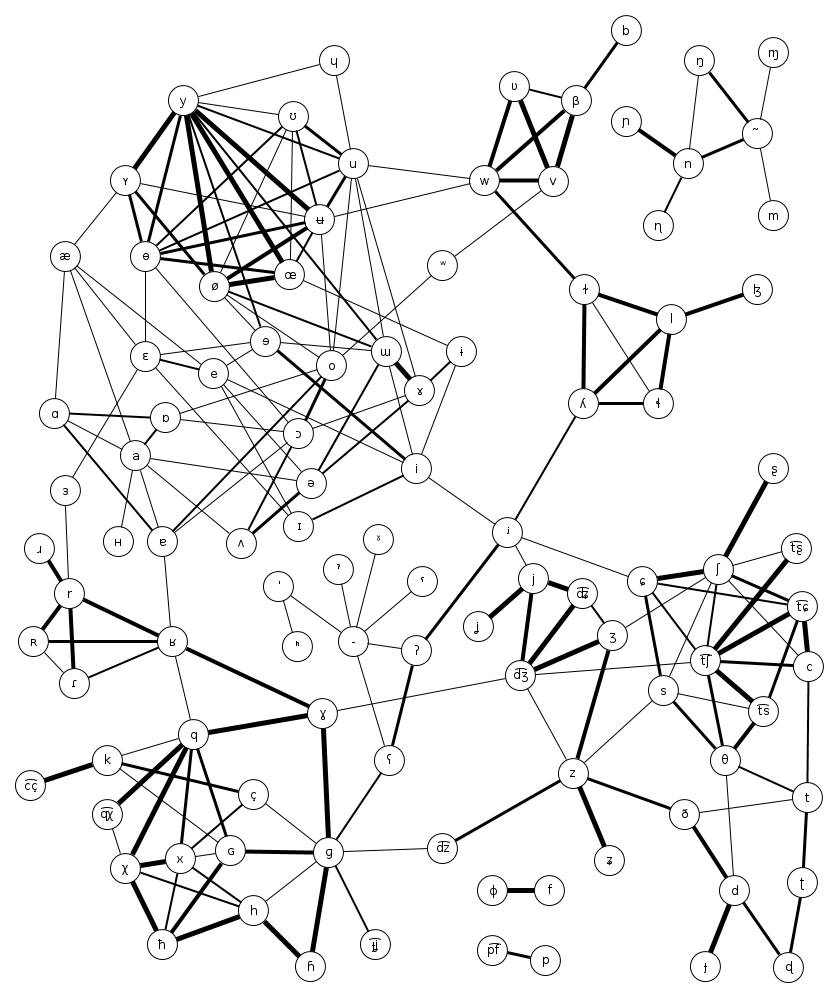
\includegraphics[width=\textwidth]{figures/phoneme-neighbor-graph.png}
\caption{Visualization of phoneme similarity as inferred from the NorthEuraLex data}
\label{fig:phonemDistGlobal}
\end{figure}

After iterating the scoring scheme three times in order to include more distant cognates based on rough earlier approximations, the result derived from a final number of more than 300,000 good cognacy candidate pairs in NorthEuraLex is visualized in \figref{fig:phonemDistGlobal}. All segment distance scores lower than 0.5 are visualized as links, and the thickness of the lines represents the similarity of the segments. A perhaps more readable representation of global sound segment correspondences was given in the overview of the IPA inventory already, where the neighbors are sorted by ascending distance, and distances between 0.5 and 0.6 are additionally given in gray color. The asymmetry in some of the neighbor relations is due to the fact that values vary slightly with the random permutations used for estimating $\hat{c}(a,b)$. In tests, this slightly non-deterministic behavior remained even for 100 resamples, and only has negligible effects in later computations.

\subsection{Inferring pairwise correspondences for NorthEuraLex}
To infer sound correspondence models for each pair of languages, we repeat the procedure that we
used for inferring the global sequence similarities on cognate pairs for that language pair.
The core idea is that if strong sound correspondences are found, they will represent the
type of correspondences we can expect in true cognates. Because the local model for unrelated
languages will not find any correspondences beyond random noise (or at least, the signal will
be weaker than the global sequence similarities), we need to maintain the global correspondences
in order to find loanwords between unrelated languages. This motivates the design choice
to define the combined distance $d(s_1,s_2)$ between two segments as the minimum
of the global distance $d_{glo}(s_1,s_2)$ and the local distance $d_{L_1,L_2}(s_1,s_2)$.
In this, the architecture presented here differs significantly from the approach implemented
in LingPy, where the alignment scores are based on a mixture of global and pair-specific
correspondence scores, and not the minimum.

We conclude the discussion of sound correspondence inference by taking a closer look at the inferred correspondences for several language pairs. \figref{fig:driftGraphEnDe} visualizes the inferred correspondences between \ili{English} and \ili{German} in the form of what I will call a \textit{\isi{drift graph}}. Between all the IPA segments present in one language, we visualize all segment distances below a value of 0.5, and use the thickness of lines to represent segment similarity. Global correspondences which were not strengthened by inference of correspondences remain in black, whereas green arrows represent correspondences which were strengthened from the perspective of the first language. The arrows can thus be read as the regular sound changes which would be inferred under the assumption that the first language developed into the second one.

For \ili{English} and \ili{German}, most sound correspondences are inferred correctly. For instance, English [p], while corresponding to German [p͡f] in most contexts, often corresponds to [f] due to subsequent simplification, as can be seen in examples such as the cognate pairs \textit{ripe} and \textit{reif}, \textit{sharp} and \textit{scharf}, and \textit{sheep} and \textit{Schaf}. Also, an apparent chain shift [ð] $\rightarrow$ [d] $\rightarrow$ [t] $\rightarrow$ [t͡s] becomes very clearly visible. The detected shifts correctly represent the High German consonant shift which occurred in the southern parts of the West Germanic dialect continuum, giving rise to \ili{Old High German}. Other prominent correspondences include [s] $\rightarrow$ [z] (as in \textit{sun} [sʌn] vs. \textit{Sonne} [zɔnə]), [v] $\rightarrow$ [b] (as in \textit{give} [ɡɪv] vs. \textit{geben} [ɡeːbən]), and [w] $\rightarrow$ [v] (as in \textit{water} [wɔːtə] vs. \textit{Wasser} [vasɐ]).

\begin{figure}
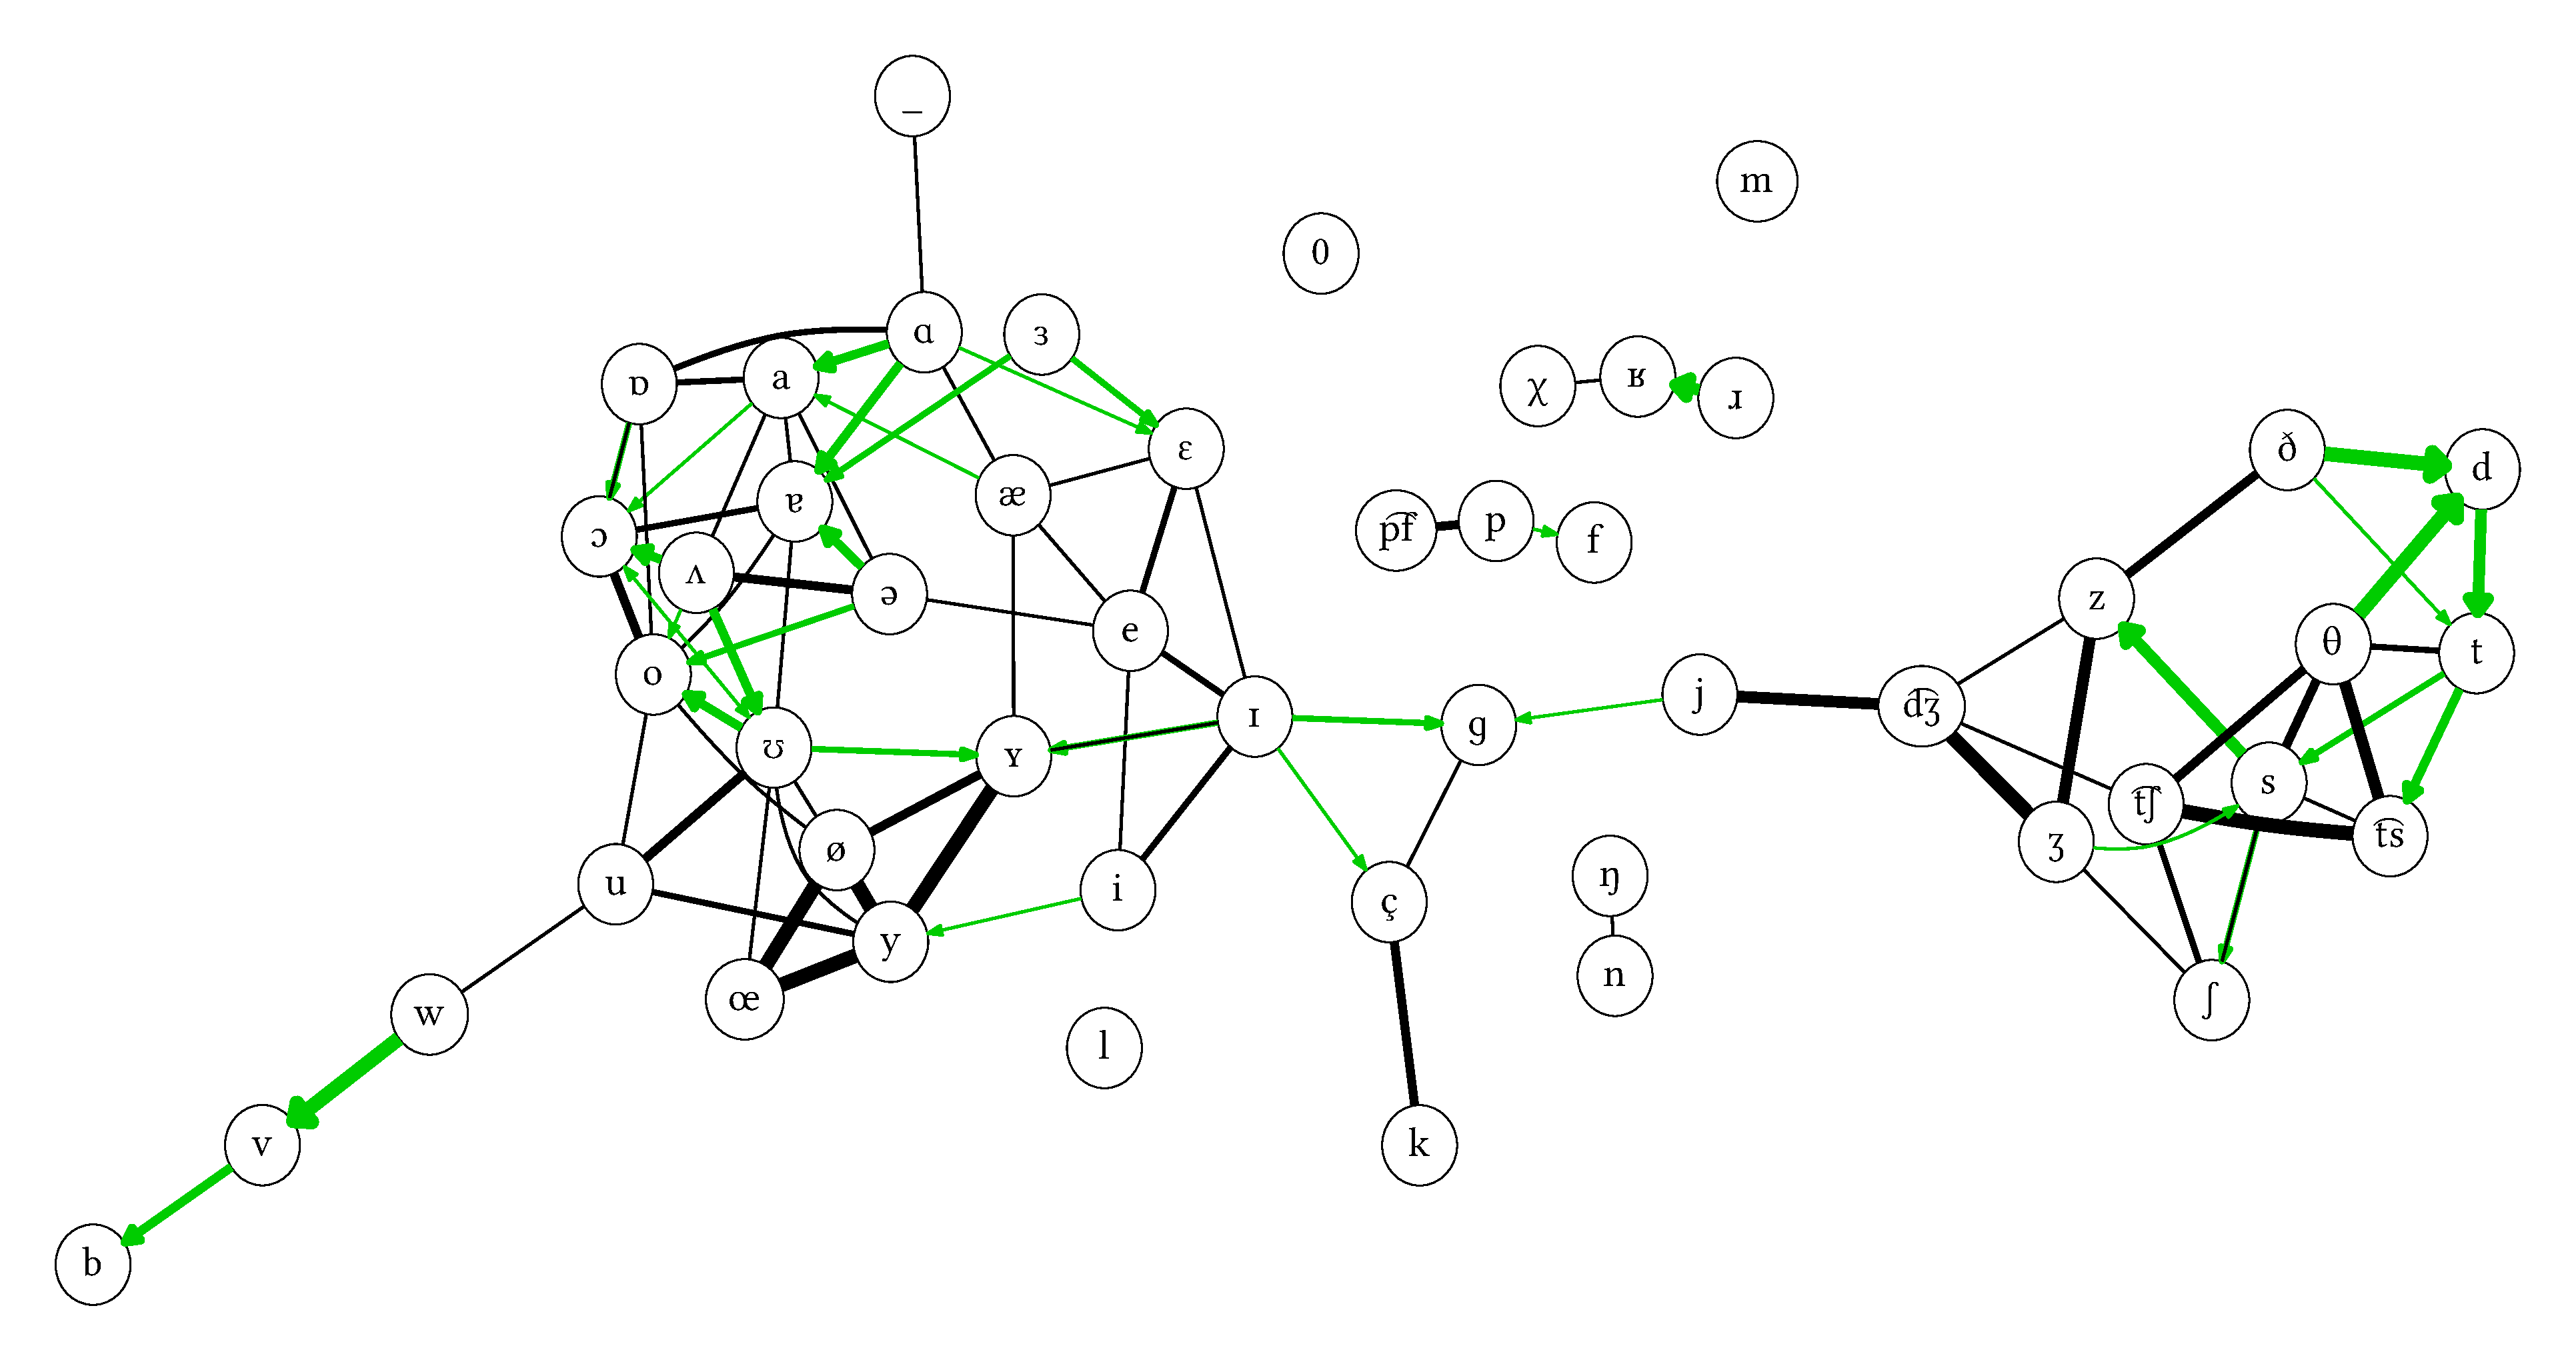
\includegraphics[width=\textwidth]{figures/drift-graph-en-de.pdf}
\caption{Drift graph of inferred correspondences from English to German}
\label{fig:driftGraphEnDe}
\end{figure}

Turning to another pair of closely related Indo-European languages, we take a look at the drift graph from \ili{Lithuanian} to \ili{Latvian} in \figref{fig:driftGraphLtLv}. Here, we have some very prominent correspondences without which an automated system would fail to find many cognates even between this closely related pair of languages. The three most prominent correspondences are Lithuanian [k] and Latvian[t͡s], (reflected in cognate pairs such as \textit{kepti/cept} `to bake' and \textit{lokys/l\={a}cis} `bear'), Lithuanian [ɡ] vs. Latvian [d͡z] (as in \textit{giesm\.{e}/dziesma} `song' or \textit{gyventi/dz\=ivot} `to live'), and Lithuanian [ʋ] vs. Latvian [f] (due to devoicing in Latvian in pairs such as \textit{t\.{e}vas/t\={e}vs} `father' or \textit{\v{z}uvis/zivs} `fish'). There is a problematic (though weak) correspondence between [n] and [ɔ]. Inspection of the alignments shows that this happens in cognates where Lithuanian \textit{an} [ɐn] corresponds to Latvian \textit{o} [uɔ] (also reflecting ancestral \textit{*an}) in word pairs such as \textit{ranka/roka} `hand' and \textit{antras/otrais} `second', which cannot be modeled by single-segment correspondences.

\begin{figure}
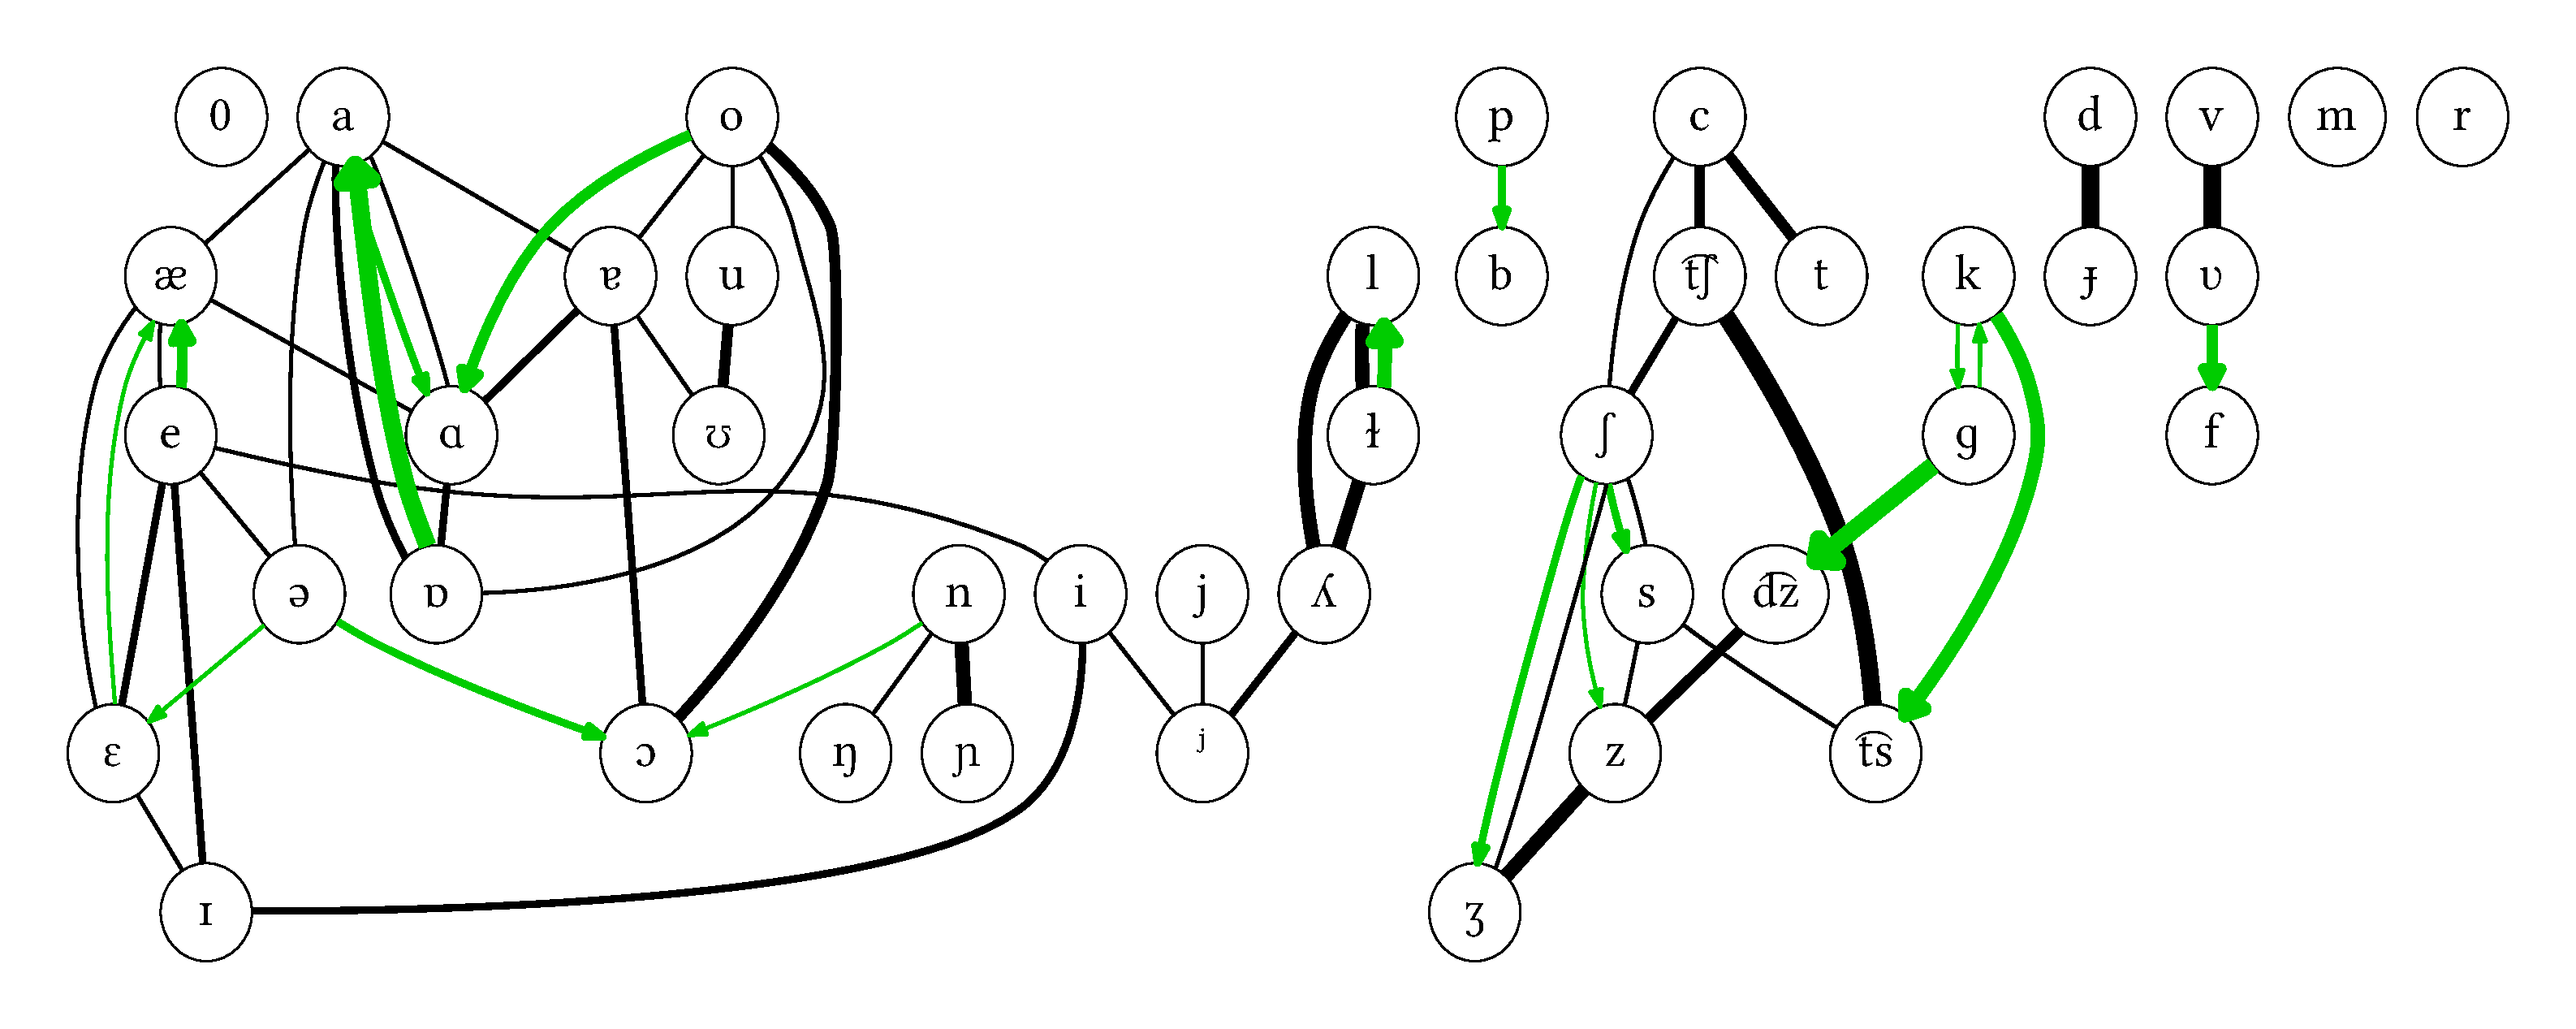
\includegraphics[width=\textwidth]{figures/drift-graph-lt-lv.pdf}
\caption{Drift graph of inferred correspondences from Lithuanian to Latvian}
\label{fig:driftGraphLtLv}
\end{figure}

Moving to a second language family, we inspect the drift graph from \ili{Finnish} to \ili{Northern Saami} in \figref{fig:driftGraphFiSe}. While some of the inferred shifts make a lot of sense, we quickly notice that some of the inferred correspondences are a lot less plausible than the examples we have seen so far. For instance, there are weak correspondences [ɛ]/[ʃ] and [n]/[c] which seem completely out of place. Inspection of the relevant alignment pairs shows that much like in the case of the erroneous correspondence between Lithuanian and Latvian, these patterns are due to non-root segments. Some Finnish nouns in \textit{-e} which historically ended in \textit{*-ek} are cognate with Northern Saami nouns in \textit{-a\v{s}}. Examples in the NorthEuraLex database include \textit{murhe/mora\v{s}} `sorrow', \textit{perhe/beara\v{s}} `family', and \textit{k\"a\"arme/gearpma\v{s}} `snake'. The reasons for the erroneous inference of [n]/[c] are more subtle. Relevant pairs include \textit{sanoa/dadjat} `to say' and \textit{huono/headju} `bad'. In both of these cases, Saami \textit{dj} [cc] overlaps in alignments with Finnish \textit{n}, a situation which occurs too often to be attributable to chance, and is therefore resolved by matching the Finnish [n] with one of the [c] sounds of the Saami geminate.

\begin{figure}
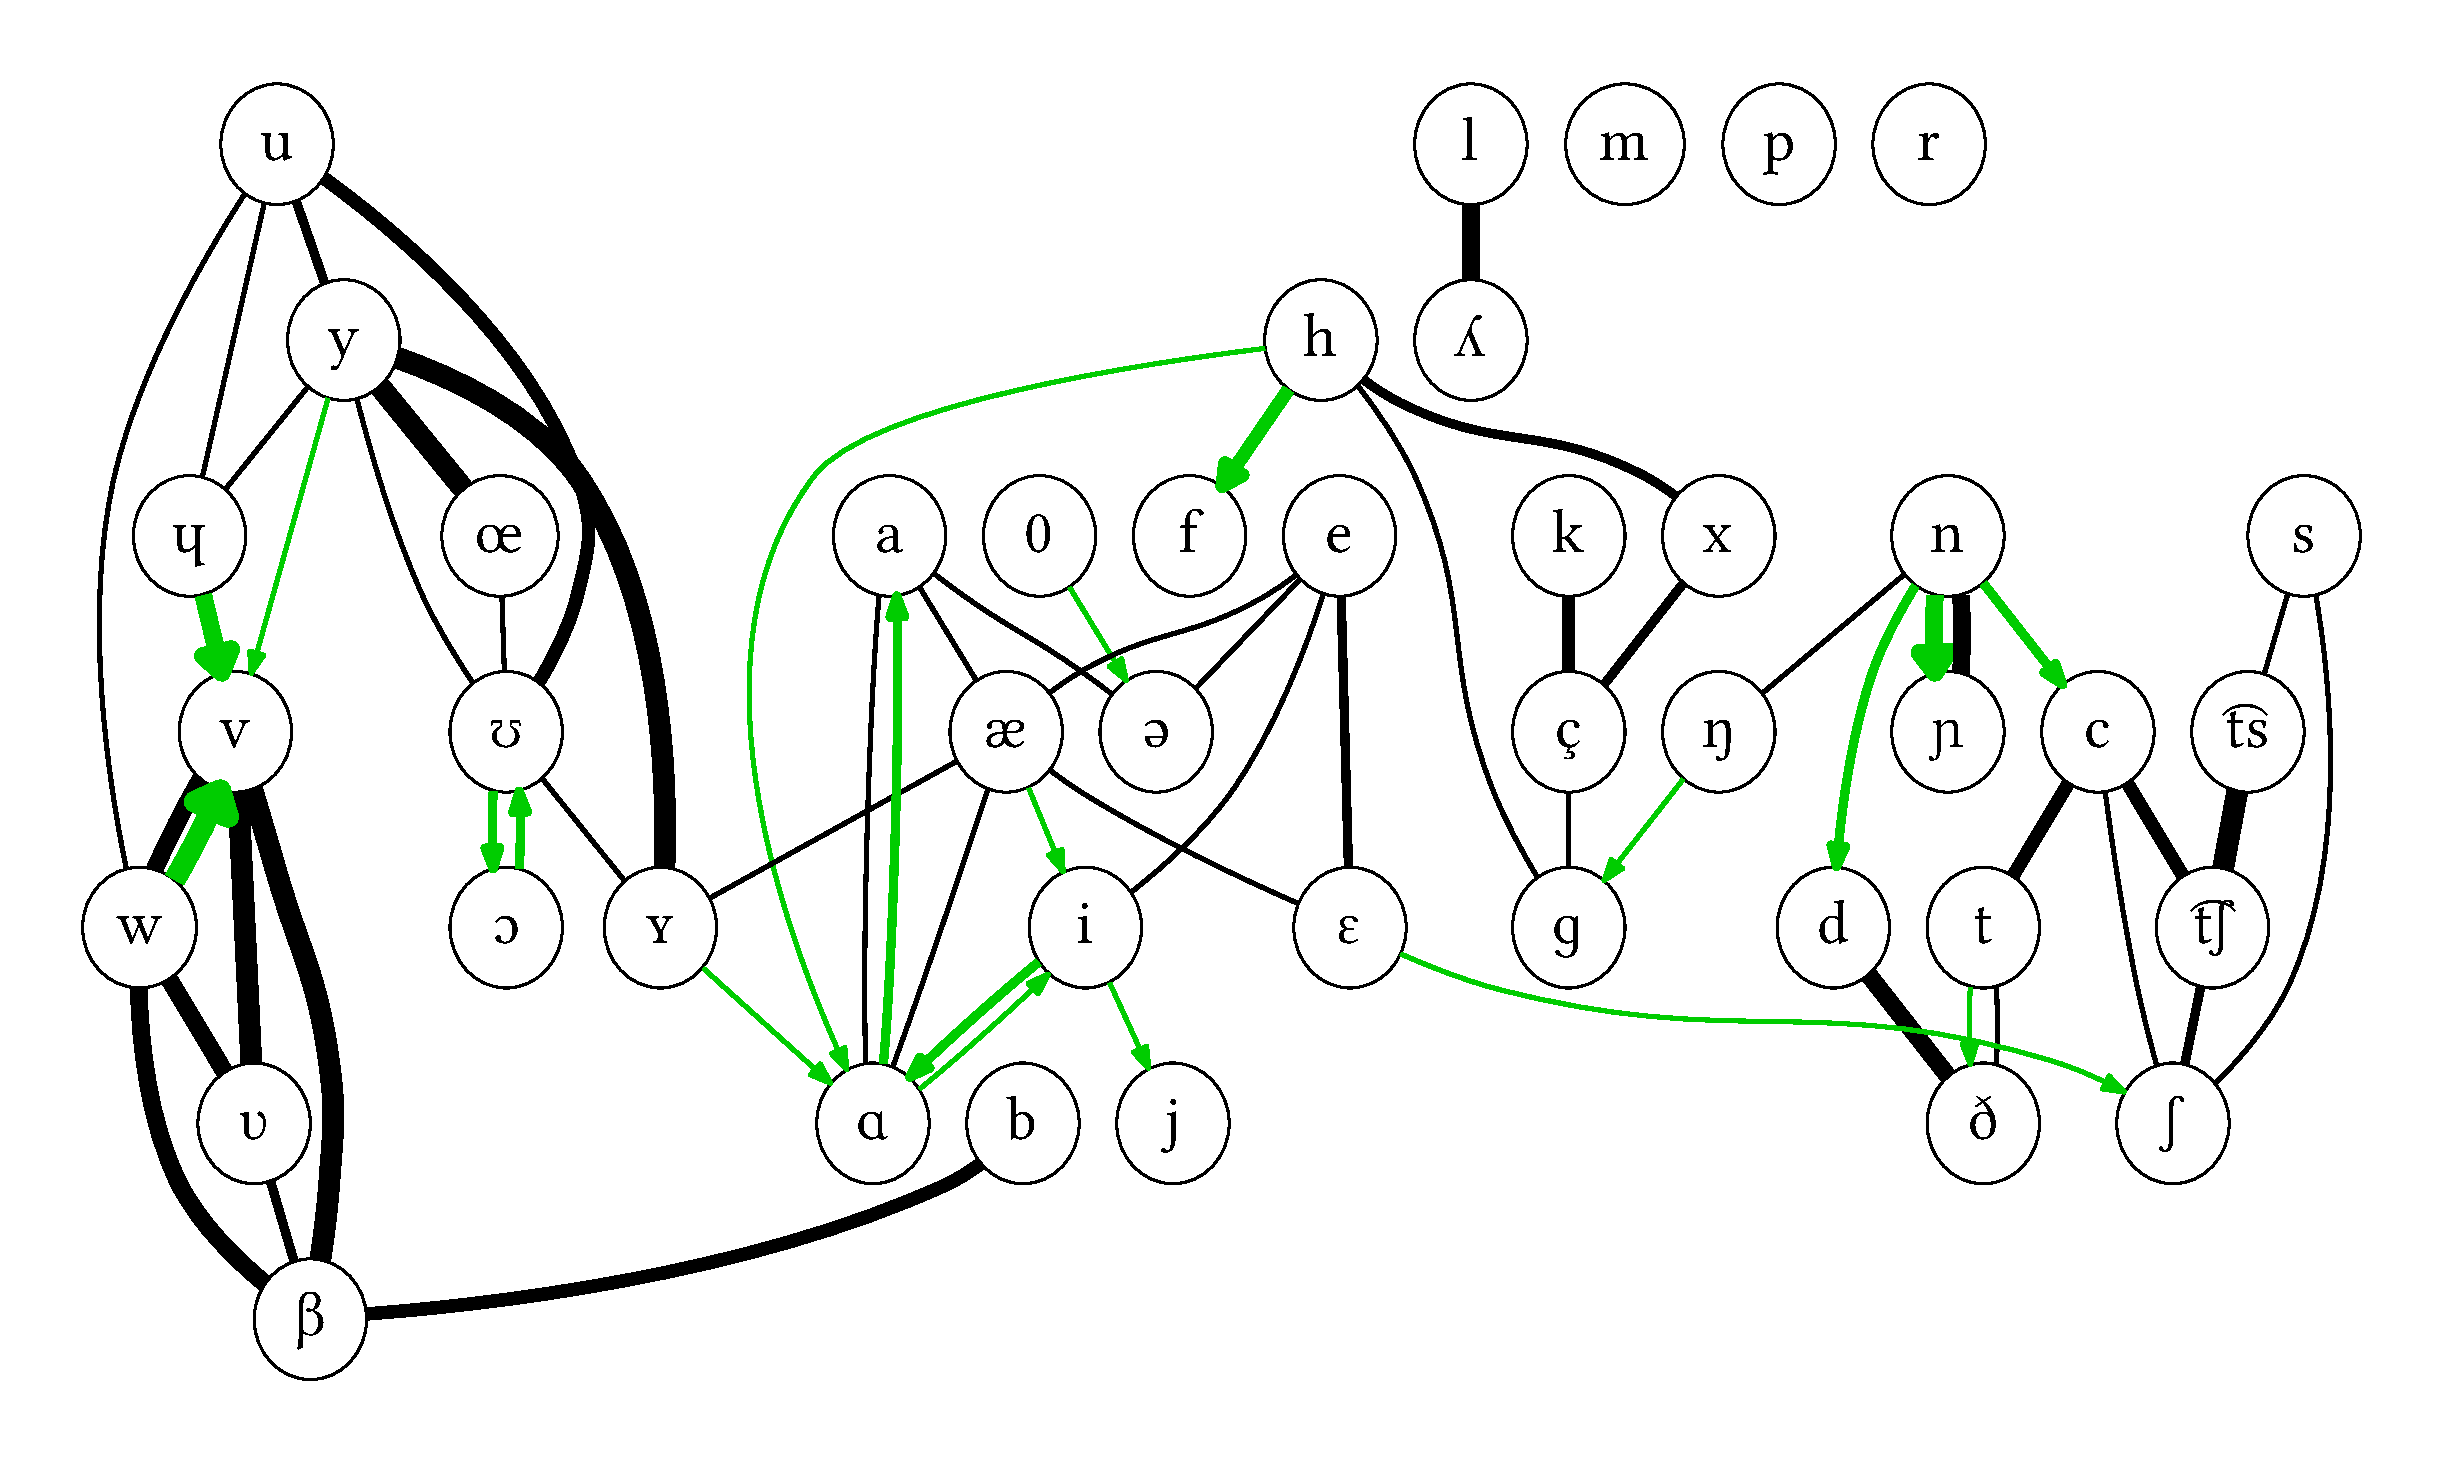
\includegraphics[width=\textwidth]{figures/drift-graph-fi-se.pdf}
\caption{Drift graph of inferred correspondences from Finnish to Northern Saami}
\label{fig:driftGraphFiSe}
\end{figure}

Much more difficult to recognize, due to the low number of cognates, are the major sound shifts which separate \ili{Finnish} from \ili{Hungarian}. The relevant drift graph in \figref{fig:driftGraphFiHu}, however, still clearly shows two of the major sound shifts which occurred in the history of Hungarian. The correspondence [k]/[h] is correctly inferred from cognate pairs such as \textit{kala/hal} `fish' and \textit{kuulla/hall} `to hear', and the correspondence [p]/[f] covers pairs such as \textit{puu/fa} `tree' and \textit{p\"a\"a/f\H{o}} `head'. The vowel correspondences are a lot more chaotic, and also less well-represented, leading to fewer local correspondences among vowels, except a tendency to map Finnish \textit{e} [ɛ] to Hungarian \textit{\'e} [e], due to cognate pairs such as \textit{pes\"a/f\'eszek} `nest', and a mapping of the vowel [u] (much more frequent in Finnish than Hungarian) to [ɒ], which is very frequent in Hungarian, but does not occur
in Finnish. The mapping of Finnish \textit{\"a} [æ] to the gap symbol is mainly due to the fact that an overwhelming majority of dictionary forms of Finnish words ends in a vowel, whereas Hungarian has undergone a process of monosyllabification (as evidenced in some of the examples above). The purpose of the cheap vowel-to-gap mappings for modeling Finnish-Hungarian cognates is therefore to reduce the costs of deleting the trailing vowel from the Finnish lexemes, which contains little information that would be relevant for comparison with Hungarian.

\begin{figure}
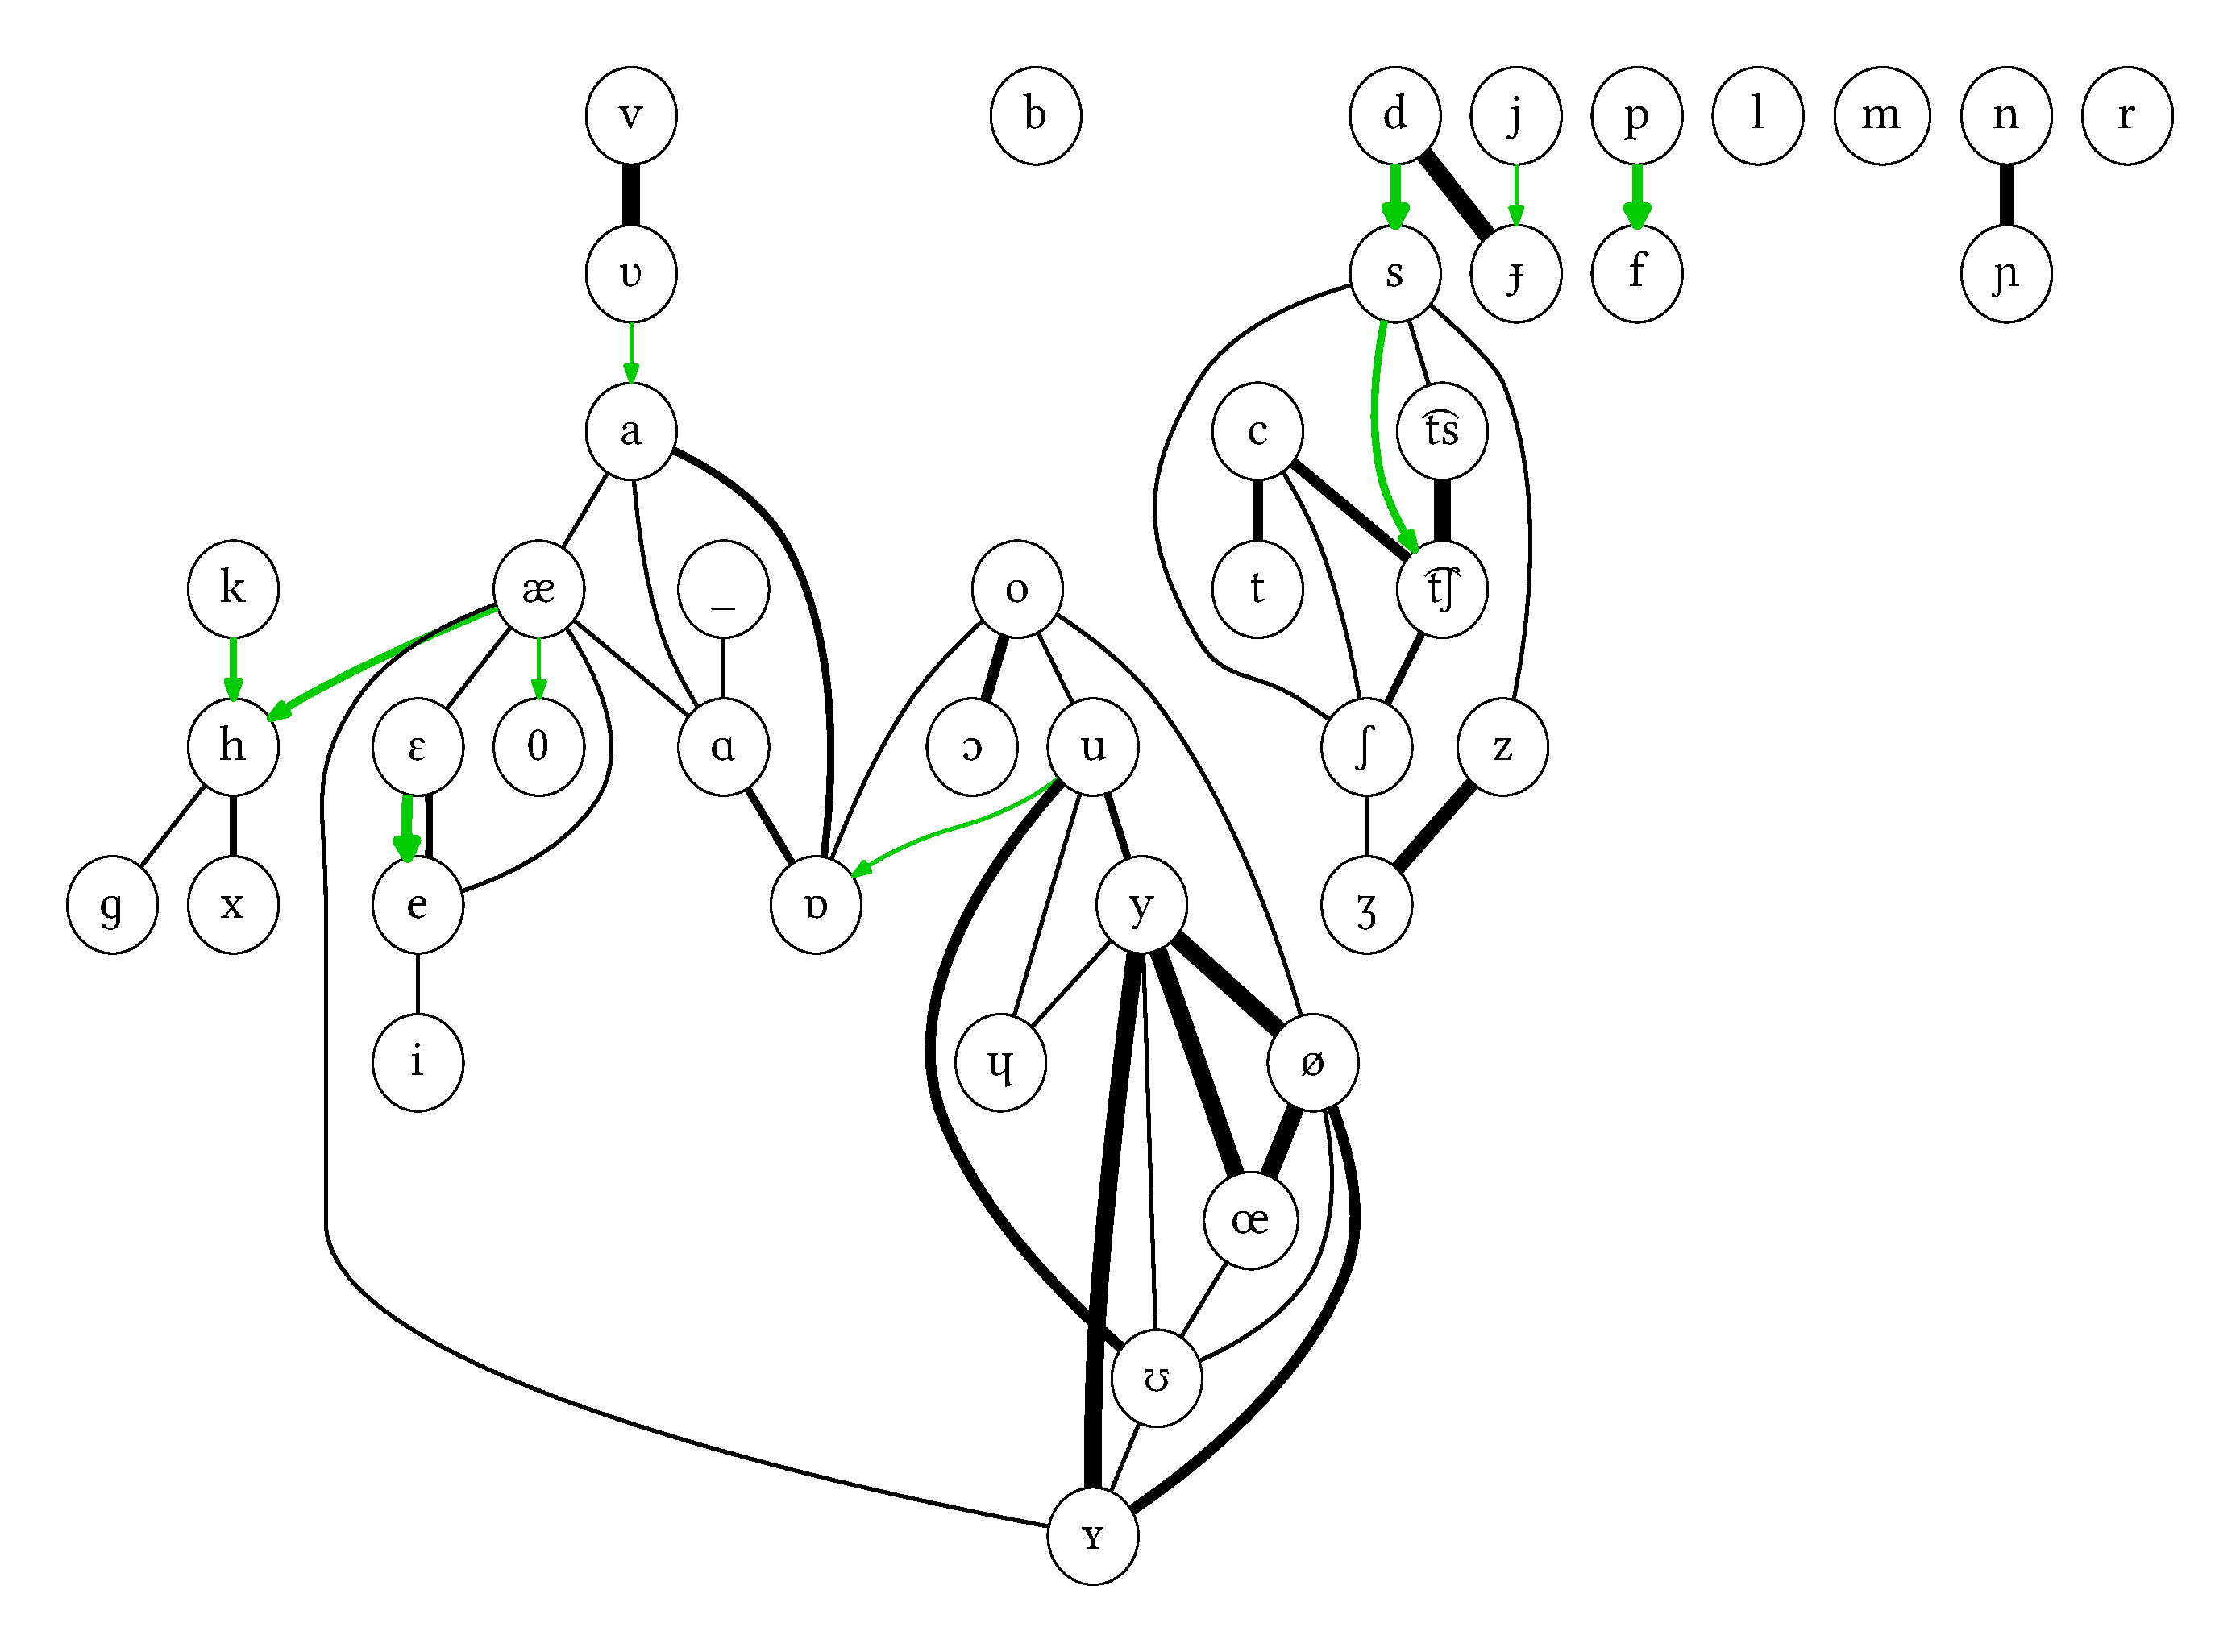
\includegraphics[width=\textwidth]{figures/drift-graph-fi-hu.pdf}
\caption{Drift graph of inferred correspondences from Finnish to Hungarian}
\label{fig:driftGraphFiHu}
\end{figure}

Finally, to illustrate that no local sound correspondences are inferred for a typical pair of unrelated languages, the drift graph from \ili{Basque} to \ili{Nivkh} is given in \figref{fig:driftGraphEuNiv}. As expected, we see almost no green arrows in this drift graph, and the two arrows which do exist are very thin, indicating only small changes to the phoneme distances. Here, the spurious correspondence [i]/[c] is due to the fact that a large class of Basque verbs ends in \textit{-i}, whereas the dictionary form of the Nivkh verb virtually always ends in \textit{-t'}, which is pronounced [c]. Without information weighting detecting and modeling that these elements are not very informative, the effect of this systematic pattern would have been much stronger. The [s]/[h] correspondence is due to the low frequency of word-initial [h] in Nivkh and the high frequency of [s] (written \textit{z}) in Basque, combined with a handful of spurious similarities such as \textit{azal} and \textit{hal} `skin'.

\begin{figure}
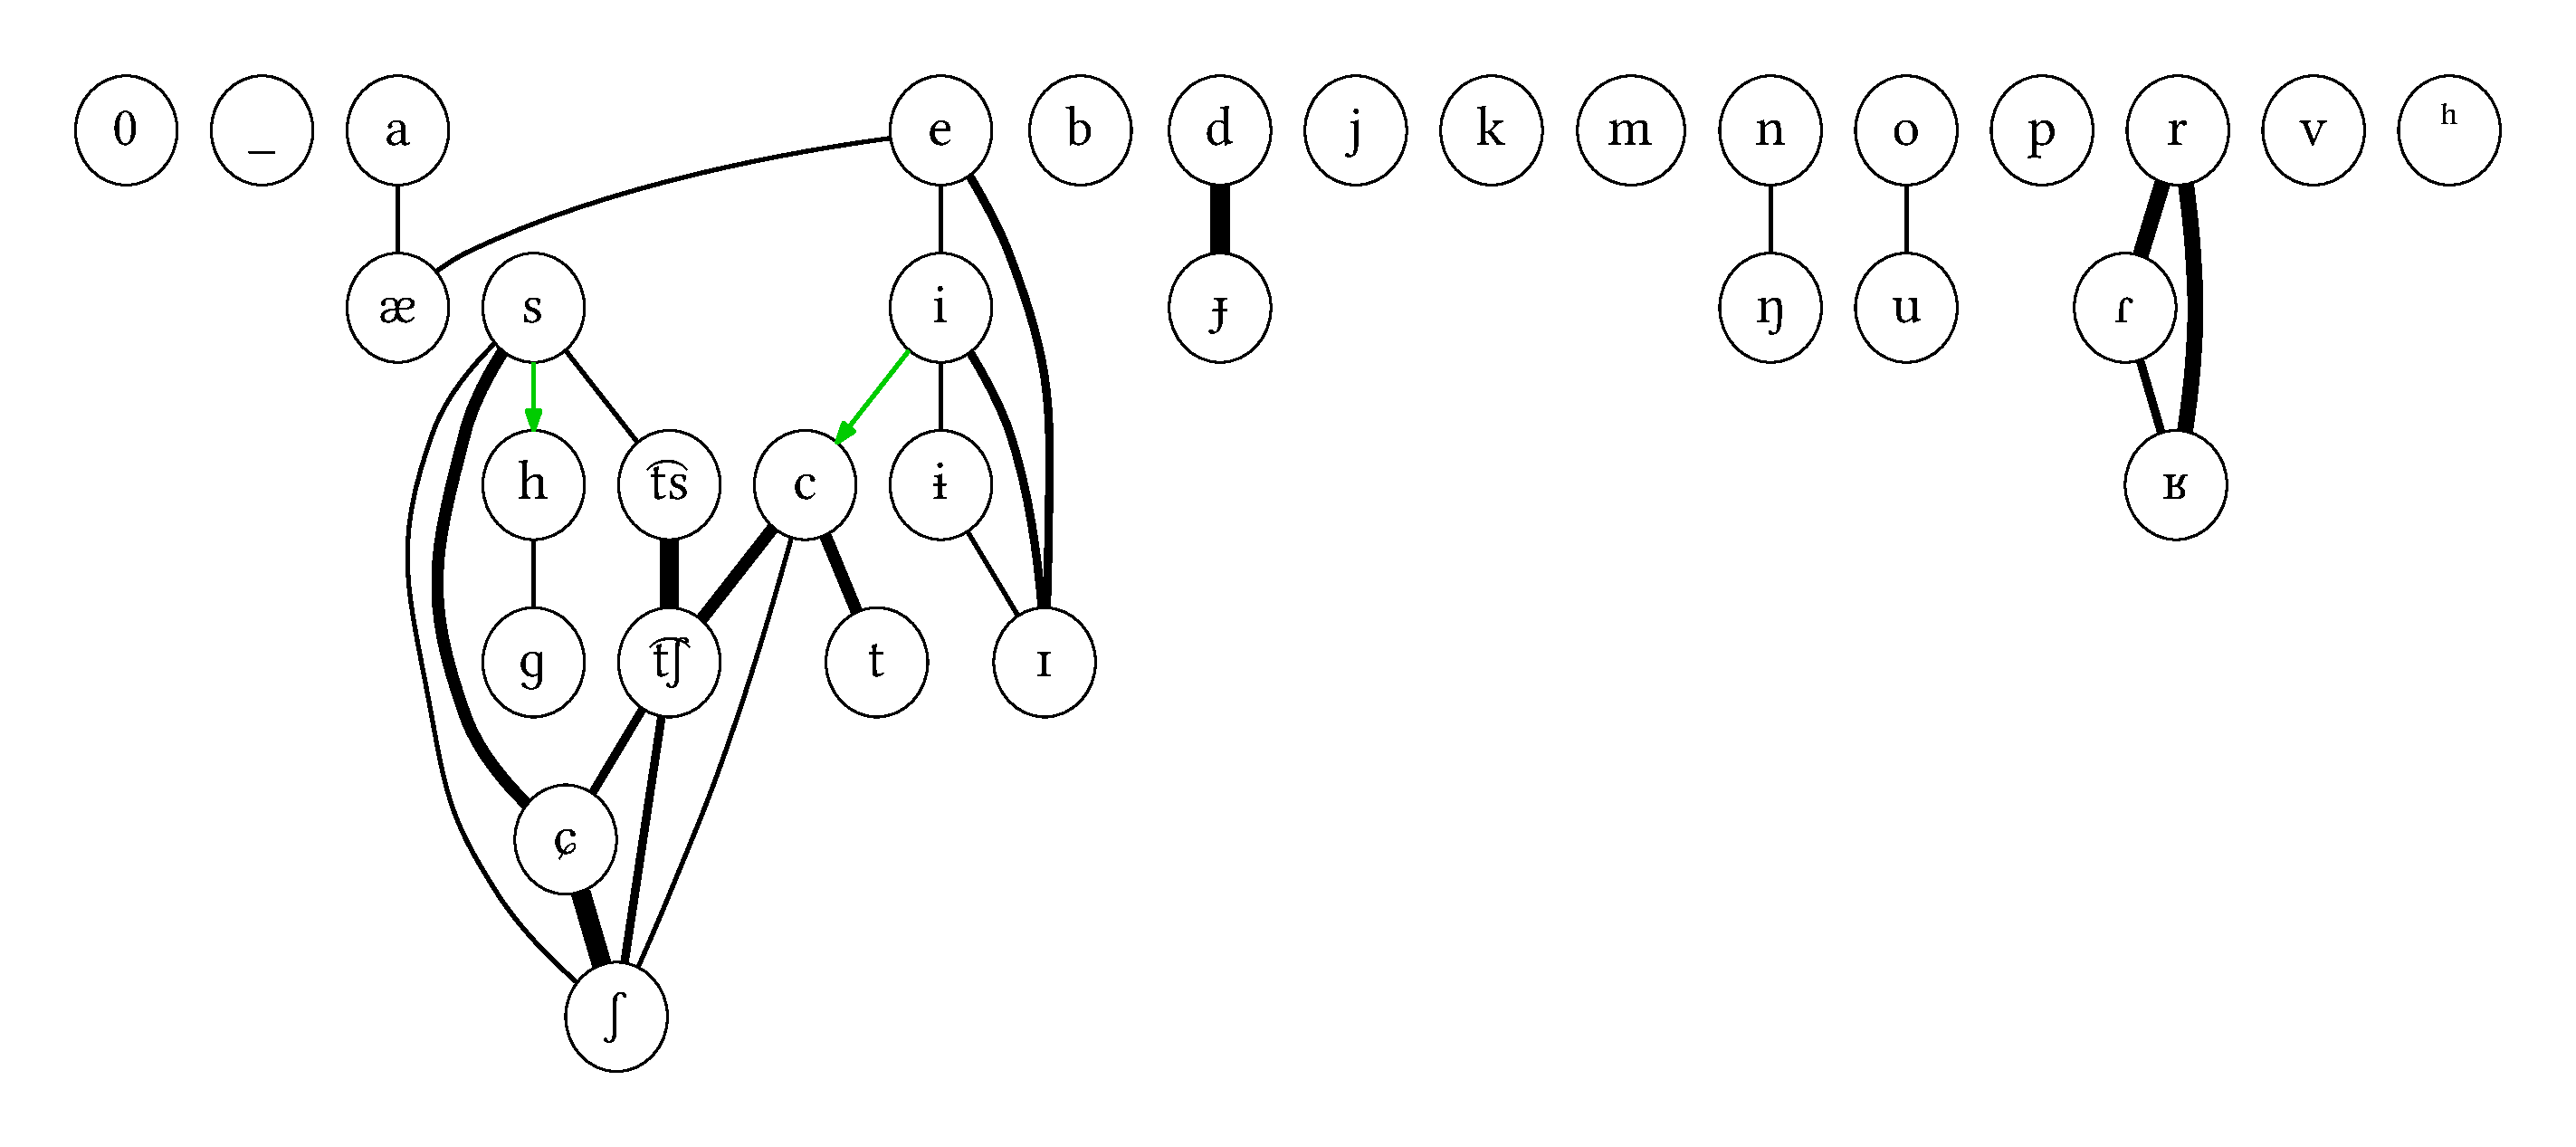
\includegraphics[width=\textwidth]{figures/drift-graph-eu-niv.pdf}
\caption{Drift graph of inferred correspondences from Basque to Nivkh}
\label{fig:driftGraphEuNiv}
\end{figure}

\subsection{Aligning NorthEuraLex and deriving form distances}

Unlike the LexStat sequence distance by \cite{list2012}, IWSA does not need to be modified by using an end-space free variant of the dynamic programming algorithm, because recurrent prefixes and suffixes are treated by the information weighting, and compounds must not be treated as full cognates. For a recent treatment of partial cognacy, the case I am avoiding, the reader is referred to recent work on detecting partial cognacy by \cite{list_ea_2016}.

The main building block of my procedure for deriving form distances from NorthEuraLex is thus IWSA on word class-specific information models, combined with a scoring scheme which maps both global and pair-specific phoneme distance scores onto $[0,1]$ by cutting off extreme values of mutual information.

\section{Cognate clustering}\label{sec:4.5}
The final step in the pipeline from raw phoneme sequence data to an estimate of cognate sets is to derive cognate sets from the normalized sequence distances. For this step, I will not attempt to introduce any new ideas. Instead, this section gives an overview of current approaches to the cognate clustering problem, and motivates the use of a comparatively well-established method for the purposes of my research.

\subsection{The cognate detection problem}
The binary cognacy judgments problem can be simplified considerably by exploiting the fact that cognacy judgments should be transitive, i.e.\ if we assume a pair of words $w_1$ and $w_2$ to be cognates, and a third word $w_3$ to be cognate with $w_2$, we must also assume that $w_1$ and $w_3$ are cognates. Mathematically, this reduces a solution to the cognate detection problem to a partition $W = W_1 \uplus W_2 \uplus \dots \uplus W_n$ of a set of phonetic strings $W$, such that $w_i$ and $w_j$ represent words with a common ancestor iff $w_i,w_j \in W_k$ for one of the sets $W_k$. From an algorithmic perspective, deriving such a partition is a clustering problem, for which well-defined solutions exist if there is a distance matrix which defines the dissimilarity between each pair of data points. This is the approach taken by practical solutions to cognate clustering, at least as a final step.

\subsection{Approaches to cognate clustering}
A very quick and simple method for cognate detection was proposed by \cite{turchin_ea_2010}, who reduce the phonetic forms to nine consonant classes of roughly the same granularity as the Dolgopolsky classes, and approximate cognacy judgments by defining two words to be cognate iff the first two consonant classes are identical. The binary judgments are not explicitly used to create cognate sets, because the authors are only interested in statistical evidence of language-wide long-distance relationships. Still, a definition based on identity is trivially transitive, turning this into a very quick and at least partially linguistically motivated way of partitioning a list of phoneme sequences into rough cognate classes.

We now come to the more mainstream approaches, where some distance matrix between surface forms is given. On data of this type, a wide range of well-understood clustering algorithms can in principle be used to derive cognate sets. Popular algorithms include hierarchical (i.e.\ tree-building) clustering algorithms such as single-linkage clustering, complete linkage clustering, and UPGMA \citep{sokal_michener_1958}. Centroid-based clustering algorithms such as k-means clustering \citep{lloyd1982} are only of very limited use to this application, because we do not have an explicit feature representation of the objects (put differently, the objects are not explicitly represented as vectors in a space). While kernelized variants of some clustering algorithms could in principle be used, the usage of clustering algorithms which operate on the level of single links is much more natural on data which comes in the shape of a distance matrix.

Hierarchical clustering algorithms are the most obvious choice for a task where we have nothing more than distance values for all pairs of objects. For instance, UPGMA derives a hierarchical clustering (a tree) over the data points by iteratively adjoining the element that has the smallest average distance to one of the existent clusters (= subtrees) as a sister node to the head of that subtree. To derive a partition into cognate sets from such a hierarchical clustering, all one needs to do is to stop the process at a user-defined threshold value before the entire tree is constructed, and to treat the subtrees created so far as cognate sets. Since the output of this variant does not include a tree structure, it is called flat UPGMA.

The disadvantage of any hierarchical clustering method is that it is difficult to avoid chaining effects, where very distant points are erroneously clustered together through a dense chain of intermediate points which build a bridge between the two distant points. Since no alternative clustering paradigm is without such weaknesses, UPGMA remains the default method for deriving cognate clusters from form distance matrices. For instance, the cognate clustering in LingPy is implemented by running UPGMA up to a user-defined threshold on user-definable form distances, the default being the distances inferred by LexStat or SCA.

Moving beyond UPGMA, attractive alternative clustering algorithms for the cognate detection task have recently been found in the community detection literature. Community detection algorithms can be applied to cognacy detection by creating a node for each word form, and connecting all pairs of forms below a certain distance threshold. In the algorithms which operate on weighted networks, the weights of the connections can be defined from the form distances. The communities found in the network, subgraphs which are in some sense more strongly connected internally than to other parts of the graph, can then be interpreted as representing cognate clusters.

Among community detection algorithms, label propagation\is{label propagation algorithm} by \cite{raghavan_ea_2007} is conceptually the most simple, and it is also very efficient because it is based on local update decisions. The core procedure of the unweighted variant is to start with a unique label on each node, and then to iteratively reassign the labels, letting each node adopt the label shared by most of its neighbors. In situations where there is no single such label, the new label is selected through uniform sampling among the best options. The process is stopped once every node has at least as many neighbors with its current label as with any other label. As the authors show, nodes with identical labels agree very well with the community structure in several interesting types of networks. While label propagation has the advantage of avoiding chaining effects, it has a problematic tendency to assign every node to one of the larger clusters, leading to quite a few false positives if some words do not
have any cognate in the input set.

The InfoMap community detection algorithm\is{InfoMap algorithm} by \cite{rosvall_bergstrom_2008} tends to perform better in this respect, and has therefore gained some traction in the field as a useful alternative to UPGMA. InfoMap is based on sampling random walks through the network to derive a representation of information flow. Concepts of information theory are used to map partitions into two-level encodings for random walks, where efficient encodings lead to shorter descriptions of the random walks. Using general optimization techniques to derive a partition whose two-level encoding minimizes the expected description length of a random walk, the algorithm infers a macro-structure which compactly represents the network, and can be interpreted to reveal the community structure.

Very recently, \cite{list_ea_2017} compared the performance of Turchin's criterion as well as UPGMA on edit distance, UPGMA on SCA distance, UPGMA on LexStat distance, and InfoMap on LexStat distance, on a reasonably wide range of single-family datasets contributed by experts. Surprisingly, they find that the accuracy across all the approaches only varied between 82\% and 89\%, with LexStat performing best, and a very slight advantage for InfoMap clustering over UPGMA. \cite{rama_ea_2017} combine PMI-based distance scores with InfoMap clustering, and evaluate the resulting system on a range of datasets against LexStat, as well as an alternative distance score derived from Pair Hidden Markov Models (PHMM). On a range of test sets, they find that PMI scores trained in an unsupervised fashion using online expectation-maximization, in combination with the Needleman-Wunsch algorithm and InfoMap clustering, beat LexStat by a small margin on a number of datasets. On average, both LexStat and their best system are
again not much better than normalized Levenshtein distance (0.819/0.842 vs. 0.804) in the B-Cubed F-score measure used by both papers to measure accuracy. It therefore seems relatively easy to achieve a quite respectable performance using any method, while improving on the already good baseline performance of simple methods appears to be quite difficult. From the perspective of a historical linguist, it is at least promising to see that the correspondence-based LexStat distances and PMI-based distances come out on top across approaches and datasets.

Within the machine learning paradigm, cognate detection can alternatively be viewed as a binary classification problem. This implies using test data to let a system learn to make correct binary decisions (cognate or non-cognate) for pairs of words. Early work in this direction is summarized by \cite{rama2015}, who trains a Support Vector Machine (SVM, a mainstream model in machine learning) over a feature representation that encodes shared subsequences, and shows that this feature set outperforms earlier SVM-based attempts. Moving to non-linear classifiers, \cite{rama2016} applies a convolutional neural network (CNN) on handcrafted representations of ASJP data, and shows that this approach is quite successful at deciding cognacy between pairs of words from smaller families. Unfortunately, the results are not compared to other approaches outside the binary classification paradigm.

Since the results of pair-wise classification will typically not lead to a consistent result (as the cognacy relation is transitive, whereas binary decisions taken in isolation will typically not be), it will typically need to be combined with an additional clustering stage in order to arrive at a partition into cognate sets. This is the approach taken by \cite{jaeger_sofroniev_2016}, who train an SVM to predict pairwise probabilities of non-cognacy from phonetic distances, overall language distance, and average word length, and combine the result with UPGMA clustering to derive the cognate sets. The method is reported to slightly outperform LingPy's LexStat method on the cognate clustering task, and seems to profit from better clustering methods. Given sufficient amounts of training data, supervised machine learning methods for classification have thus started to show some promising results for the cognate detection task.

Unfortunately, the way in which all these methods have so far been evaluated does not tell us much about their performance on a dataset like NorthEuraLex which spans several language families. For such multi-family datasets, it makes sense for a system to put more effort into avoiding false positives, whereas for intra-family comparison, the probability that two similar-looking words for the same concept are not cognate is very small. Since we do not yet have a cognacy-annotated subset of NorthEuraLex which spans several language families, supervised machine-learning methods are impossible to apply. Still, comparing my own IWSA-based system to LingPy provides some indication of how it would fare against these methods, given that they have so far not managed to outperform LingPy significantly.

\subsection{Deriving cognate sets from NorthEuraLex}
By using the same variant of the UPGMA algorithm as LingPy, I am opting for a well-established method for deriving cognate sets inference from form distances. To derive the threshold value for my IWSA-based distances, manual inspection of the cognate sets for a handful of concepts on different threshold values suggested 0.45 as leading to results which best fitted my knowledge about the true cognate sets in Indo-European and Uralic. Since a part of the evaluation we are going to see in the next section is threshold-independent, the empirically determined thresholds from this step will be combined with this impression to decide on the threshold value used for the cognate clustering that the following chapters will build on.

\subsection{Evaluation on IELex intra-family cognacy judgments}
As previously mentioned, the lack of fully cognacy-annotated cross-family data sets makes it difficult to quantitatively evaluate the quality of the cognacy judgments produced by my architecture. Still, it is necessary to at least test on a small subset whether the results are measurably better than the LingPy output, just as the initial inspection in the last section suggested. Also, this small subset can help us in deriving good threshold values if we systematically analyse the precision-recall tradeoff provided by threshold selection.

For this purpose, I was able to use a dataset kindly provided by Pavel Sofroniev, who created the intersection of IELex with an earlier version of the NorthEuraLex database. For the languages and concepts which are covered by both databases, the referenced word forms were manually compared and mapped to each other, producing a database of NorthEuraLex IPA strings with the cognacy annotations given in IELex. After being updated to reflect version 0.9 of NorthEuraLex, the dataset now covers 6,106 words for 185 concepts across 37 Indo-European languages, providing a very interesting test set for cognate detection that is available as part of the supplementary material for this book (see Appendix C).

To derive the LexStat distances and cognacy judgments, I converted the entire NorthEuraLex database into the tabular input format required by LingPy, doing some trivial symbol replacements until LingPy found the input to be free of errors, and running the LexStat method on the entire database, building on code by Johannes Wahle for deriving cognate sets from the ASJP-encoded version of NorthEuraLex. In this code, LingPy is called according to recommendations by Mattis List, which included setting LexStat's threshold parameter to 0.7, and letting the scorer run without preprocessing, but with many iterations. Setting the \texttt{runs} parameter to a rather large number of 1,500 yielded stable results which barely changed when adding additional iterations, and had the advantage of still being able to infer cognate sets from NorthEuraLex in under six hours on an average office machine.

The cognate sets produced by my architecture and by LingPy were then reduced by ignoring all forms which were not in the test set, and throwing away all cognate sets which contained no form from the test set. The resulting cognate sets were converted into 100,155 pairwise cognacy judgments, on which it is easy to define pairwise performance measures like precision and recall. Each pair of words which are cognate according to IELex is counted as a true positive (TP) if it ends up in the same automatically derived cognate set, and as a false negative (FN) if it is not. Assuming the cognacy judgments in IELex to be complete, any pair of words which are inferred to belong to the same cognate set, but assigned to different cognate set IDs in IELex, is counted as a false positive (FP), and any pair that is not cognate in IELex, and is also assigned to two different cognate sets by an automated system, counts as a true negative (TN).

For evaluation, we compare the performance of three form distances in terms of average pairwise precision, and select optimal threshold values for each distance by means of the precision-recall curve. The three distances we are going to infer are LexStat distances to represent the state of the art, and the mixed scores with constant information (WED) as well as with information weighting (IWD) as computed by my implementation, to measure possible improvements due to my way of inferring sound correspondences, and further improvements due to information weighting. \figref{precision-recall-curves} shows the precision-recall curves for all three distances, which visualizes the behavior of the tradeoff between precision and recall under changing threshold values. In the low-recall range (i.e. for the easy cases), LexStat is better than the other two methods, but its precision decays more quickly with higher recall. This makes IWD and WED better suited for the more difficult instances. The fact that the IWD curve is always higher than the WED curve shows the global advantage of information weighting for separating cognates from non-cognates.

\begin{figure}[ht]
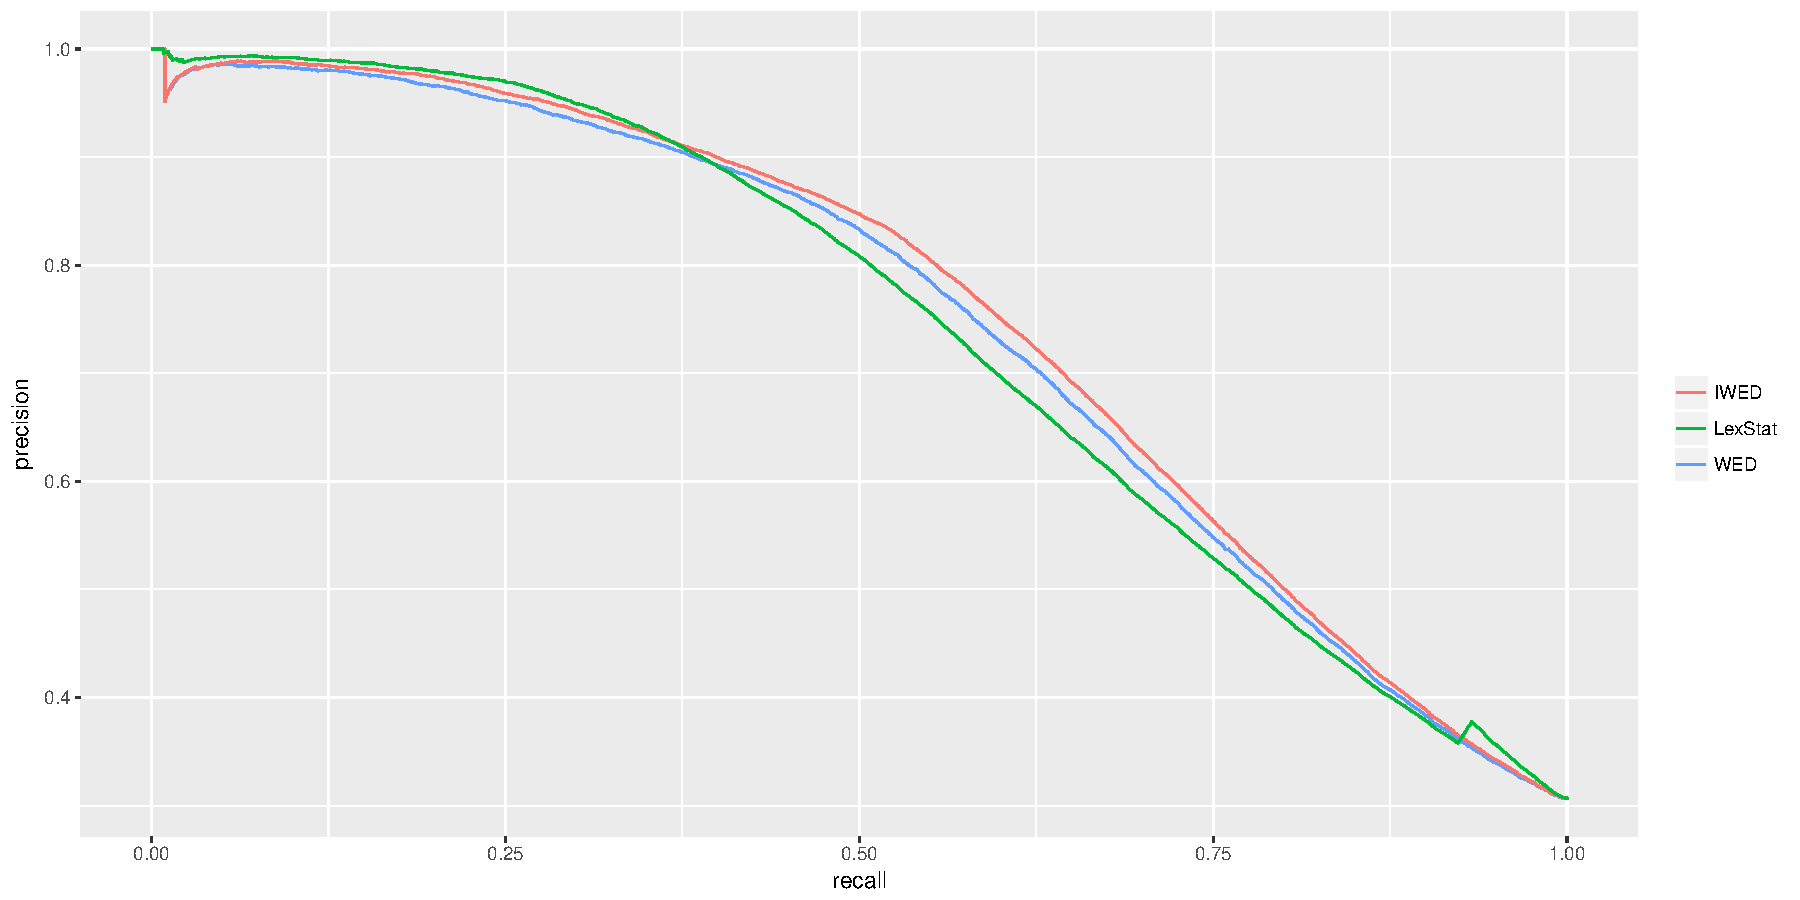
\includegraphics[width=\textwidth]{figures/precision-recall-curves.pdf}
\caption{Precision-recall curves for cognate detection variants.}
\label{precision-recall-curves}
\end{figure}

\tabref{average-precision-thresholds} includes the corresponding average precision values, which is defined as the precision integrated over all possible recall values. This gives us a possibility to quantify and compare performance independently of the choice of threshold value. According to this measure, IWD is better than WED, which in turn performs better than LexStat.

\begin{table}
\centering
\begin{tabular}{lccc}
\hline \hline
Method & LexStat & WED & IWD\\
\hline
Average Precision & 0.733 & 0.747 & \textbf{0.766}\\
\hline
Threshold for max. F-score & 0.831 & 0.590 & 0.591\\
Maximal F-score & 0.630 & 0.662 & \textbf{0.681}\\
\hline
Threshold for 85\% Precision & 0.737 & 0.495 & 0.462\\
F-score at 85\% Precision & 0.585 & 0.612 & \textbf{0.632}\\
\hline
Threshold for 90\% Precision & 0.698 & 0.430 & 0.387\\
F-score at 90\% Precision & 0.544 & 0.537 & \textbf{0.556}\\
\hline
\end{tabular}
\caption{Quantitative comparison and data for motivating the thresholds chosen for cognate detection}
\label{average-precision-thresholds}
\end{table}

The remaining entries of the table contain the necessary numbers for motivating our threshold decisions for IWD and LexStat. If we had no preference for either recall or precision, we could simply maximize the F-score. However, since spurious cognates are a lot more problematic for lexical flow than unrecognized deep cognacy, we want to select for high precision. The figure shows the threshold values corresponding to accuracy values of 85\% and 90\%, and the F-score that can be achieved by choosing that threshold value. It turns out that our initial choice of 0.45 for IWD, and the recommendation of 0.7 for LexStat, are in the range that should lead to precision in the desired range. To avoid overfitting to what also constitutes our test set, I only take this information as confirming the initial decisions, and do not optimize the threshold values further.

The already mentioned \isi{B-Cubed measures} have become the standard for cognate detection since \cite{hauer_kondrak_2011} used them for evaluation, demonstrating the usefulness of measures which go beyond pairwise comparison by taking the inferred clusters into account. For a single word, a recall measure can be defined as the percentage of gold-standard cognates (including the word itself) which occur together with the word in the same result cluster, and an analogous precision measure for each word as the percentage of words in the result cluster which are cognates to the word according to the gold standard. B-Cubed precison and recall are the averages of these clustering accuracy measures across words, and the B-Cubed F-score is again the harmonic mean of B-Cubed precision and recall. To make my results comparable to the recent literature on cognacy detection, I compute these measures in addition to the pairwise performance measures explained above.

The values of all six evaluation measures for the chosen threshold values are given in \tabref{lingpyComparisonIELex}. The numbers show an insignificant advantage of half a percentage point in B-Cubed F-score for LexStat, indicating that IWSA and LexStat perform almost exactly equally well on IPA-encoded dictionary forms for intra-family cognacy judgments. Note that this task is not the one my infrastructure is designed to be particularly good at, so that this evaluation merely shows that on dictionary forms, my system keeps up with the state-of-the-art systems for general cognate detection.

\begin{table}
\centering
\begin{tabular}{lcccccc}
\hline \hline
& \multicolumn{3}{c}{Pairwise} & \multicolumn{3}{c}{B-Cubed}\\
Method & precision & recall & F-score & precision & recall & F-score\\ \hline
IWD-0.45 & 0.927 & 0.429 & 0.586 & 0.887 & 0.518 & 0.654\\
LexStat-0.7 & 0.929 & 0.434 & 0.591 & 0.885 & 0.526 & 0.660\\
\hline
\end{tabular}
\caption{Comparing cognate clustering performance on the intersection of IELex and NorthEuraLex}
\label{lingpyComparisonIELex}
\end{table}

\subsection{Evaluation on WOLD cross-family cognacy judgments}
To conclusively demonstrate that the infrastructure presented in this chapter is better than the current version of LingPy for the purposes of cross-family cognate detection, a test set which includes cognacy judgments for a dataset which spans multiple families would be necessary. Since such datasets do not currently exist, evaluation must resort to the second-best option of complementing the family-internal evaluation provided by IELex by an evaluation on at least some cognate sets which range across family boundaries.

Fortunately, since cross-family cognates are invariably loanwords (except for a few cases where deep connections are assumed), we can rely on an existing rather comprehensive loanwords database which again has some overlap with the NorthEuraLex data. The World Loanword Database (WOLD)\is{WOLD (World Loanword Database)} was a major data collection effort coordinated by Max Planck Institute for Evolutionary Anthropology in Leipzig, the results of which are summarized in \cite{tadmor2009}. The database is available online \citep{wold}, and was published under a creative commons (CC-BY) license. It contains the realizations of a list of 1460 concepts for a geographically well-balanced sample of 41 languages, and expert judgments on the loanword status for all these words, complete with information on the sources of borrowings. There are eight vocabularies for languages also contained in NorthEuraLex 0.9: \ili{English} \citep{wold-eng}, \ili{Dutch} \citep{wold-nld}, \ili{Romanian} \citep{wold-ron}, \ili{Kildin Saami} \citep{wold-sjd}, \ili{Sakha} \citep{wold-sah}, \ili{Japanese} \citep{wold-jpn}, \ili{Mandarin Chinese} \citep{wold-cmn}, and Ket \citep{wold-ket}. Going through these WOLD vocabularies and extracting all borrowings whose donor languages (or one of their descendants containing reflexes of the same cognate set) are also contained in NorthEuraLex, were not accompanied by a semantic change, and for which the concept was covered by NorthEuraLex, resulted in an evaluation set of 414 loans within NorthEuraLex, of which 214 were intra-family loans, and 200 occurred across family boundaries. This test set is also available as part of the supplementary materials (see Appendix C), to my knowledge providing the first (if modest) benchmark for cross-family cognate detection.

Ideally, we would expect each pair of cognates defined by such a borrowing event to end up in one of the automatically inferred cognate sets. This is what the comparison of the two systems on this dataset was based on. Again, the cognate sets inferred over NorthEuraLex were reduced to a list of pairwise cognacy judgments. Since this dataset provides us with no indication which of the words not affected by borrowing are cognates or not, we unfortunately cannot sensibly compute precision values for this dataset. Instead, I will only rely on the recall values in my evaluation. For a useful comparison, it would usually be a problem if recall is not balanced against precision, but recall still provides meaningful information as long as I keep the parameters fixed, and do not further optimize the system to the new dataset. Using exactly the same system with the threshold values that I demonstrated to be on an equal footing with LingPy on the family-internal cognate classification task, I evaluate whether it manages to detect a higher proportion of cross-family loanwords.

\tabref{lingpyComparisonWOLD} shows the results of the comparison. Since loans are phonetically more similar than the reflexes of inherited cognates, it comes as no surprise that the recall values are higher than in the previous experiment. The interesting finding is in the comparion of intra-family and cross-family loans. In contrast to the IELex data, there is a clear advantage for my system on intra-family loans, probably due to the fact that LexStat requires the existence of sound correspondences, which are of course only partially adhered to by loanwords. The most significant difference is visible in the cross-family loans. Here, LingPy recognizes less than 60\% of the cross-family loans as cognates, whereas my system recognizes cognacy for almost 65\% of pairs. The reason for the difference is that LingPy's infrastructure is dependent on the existence of regular sound correspondences, which is not a problem if the task is to find true cognates within a single family, as was the case in all datasets
that LingPy has previously been evaluated on \citep{list_ea_2017}. Taking the minimum of global and pair-specific phoneme distances makes my system much more flexible in this regard, while still maintaining a competitive performance for intra-family cognate detection.

The results indicate that while for the within-family cognacy detection task, the systems show equal performance, my infrastructure seems clearly preferable for preparing cross-family cognacy datasets, the essential preprocessing step for cognacy-based lexical flow inference. In theory, my system might of course also cluster together many more cross-family non-cognate pairs than LingPy, causing precision (which we have no way of measuring) to be much lower than for LingPy, but I would consider that very unlikely given the very similar precision values on the IELex data. Still, it will of course be worthwhile to revisit this issue once larger fully annotated cross-family datasets become available, which would require massive data collection efforts on an even larger scale than the WOLD project.

\begin{table}
\centering
\begin{tabular}{lcc}
\hline \hline
method & recall on intra-family loans & recall on cross-family loans\\ \hline
LexStat-0.7 & 0.768 & 0.594\\
IWD-0.45 & 0.888 & 0.645\\
\hline
\end{tabular}
\caption{Comparing cognacy judgments on cross-family loans from the World Loanword Database (WOLD)}
\label{lingpyComparisonWOLD}
\end{table}

\subsection{A look at the cognate sets}
To illustrate the quality of the results, and the type of data hidden behind everything which is yet to follow, we inspect the NorthEuraLex data and the inferred cognate sets for the concept \textsc{fish} in detail. \figref{cognate-sets-example} contains the standardized IPA representations for all of the NorthEuraLex languages, grouped into cognate sets using UPGMA on my distance measure. I will use the given numbering from 1 to 38 to refer to the cognate sets in the discussion.

\begin{figure}[p!]
\centering \footnotesize
\begin{tabular}{clllll} \hline
1 & \texttt{gld}: [sɔɡdata] & & & & \\
\hline
2 & \texttt{kor}: [mulɡoɡi] & & & & \\
\hline
3 & \texttt{sah}: [balɯk] & \texttt{tat}: [balɤk] & \texttt{dar}: [baliq] & \texttt{bak}: [balɯq] & \texttt{chv}: [pulə]\\
& \texttt{azj}: [bɑlɯɡ] & \texttt{kaz}: [bɑləq] & \texttt{uzn}: [baliq] & \texttt{tur}: [balɯk] & \\
\hline
4 & \texttt{yux}: [ɑnil] & & & & \\
\hline
5 & \texttt{slk}: [riba] & \texttt{bul}: [riba] & \texttt{ces}: [rɪba] & \texttt{pol}: [ɾɨba] & \texttt{ukr}: [rɪbɑ]\\
& \texttt{bel}: [rɨba] & \texttt{rus}: [rɨbə] & \texttt{hrv}: [riba] & \texttt{slv}: [riiba] & \\
\hline
6 & \texttt{eus}: [arɑjn] & & & & \\
\hline
7 & \texttt{kal}: [aalisaɣaq] & \texttt{ykg}: [alʲʁa] & & & \\
\hline
8 & \texttt{evn}: [ollo] & & & &\\
\hline
9 & \texttt{heb}: [daɡ] & & & &\\
\hline
10 & \texttt{fra}: [pwasɔ̃] & \texttt{cym}: [pəsɡɔd] & & &\\
\hline
11 & \texttt{ket}: [ʊʎdʲiɕ] & & & &\\
\hline
12 & \texttt{pes}: [mɒɒhi] & \texttt{pbu}: [mɑhaj] & \texttt{hin}: [mətsj] & \texttt{mal}: [matsjam] & \\
\hline
13 & \texttt{oss}: [kəsaɡ] & \texttt{bre}: [pɛsk] & \texttt{isl}: [fɪskʏr] & \texttt{gle}: [ɪəsˠk] & \texttt{nor}: [fɪsk]\\
& \texttt{sqi}: [pɛʃk] & \texttt{dan}: [fesɡ] & \texttt{lat}: [pɪskɪs] & \texttt{swe}: [fɪssk] &\\
\hline
14 & \texttt{lit}: [ʒʊʋʲɪs] & \texttt{lav}: [zifs] & & &\\
\hline
15 & \texttt{ava}: [tt͡ʃuʕa] & & & &\\
\hline
16 & \texttt{ddo}: [besuro] & & & &\\
\hline
17 & \texttt{hin}: [mət͡ʃʰlii] & \texttt{ben}: [mat͡ʃʰ] & & &\\
\hline
18 & \texttt{hye}: [d͡zuk] & & & &\\
\hline
19 & \texttt{kat}: [tʰɛvzi] & & & &\\
\hline
20 & \texttt{bsk}: [t͡ɕʰumɔ] & & & &\\
\hline
21 & \texttt{kpv}: [t͡ɕeri] & \texttt{koi}: [t͡ɕʲeri] & \texttt{che}: [t͡ʃʼərə] & \texttt{tel}: [t͡ɕeepʌ] & \texttt{ain}: [t͡sep]\\
\hline
22 & \texttt{kmr}: [masi] & \texttt{enf}: [kari] & & &\\
\hline
23 & \texttt{mnc}: [nimaxa] & & & &\\
\hline
24 & \texttt{jpn}: [sakana] & \texttt{arb}: [samak] & & &\\
\hline
25 & \texttt{ckt}: [ənneen] & & & &\\
\hline
26 & \texttt{niv}: [cʰo] & \texttt{cmn}: [y] & & &\\
\hline
27 & \texttt{mns}: [χul] & \texttt{hun}: [hɒl] & \texttt{sme}: [kʊɔlli] & \texttt{sjd}: [kuuʎʎ] & \texttt{sma}: [kʉɛliɛ]\\
& \texttt{mrj}: [kol] & \texttt{mdf}: [kal] & \texttt{nio}: [kolɨ] & \texttt{krl}: [kɑlɑ] & \texttt{olo}: [kɑlɑ]\\
& \texttt{fin}: [kɑlɑ] & \texttt{sel}: [qælɨ] & \texttt{ekk}: [kɑlɑ] & \texttt{smj}: [ɡʊuɔllɛ] & \texttt{yrk}: [xɑʎɑ]\\
& \texttt{myv}: [kal] & \texttt{vep}: [kɑlɑ] & \texttt{mhr}: [kol] & \texttt{liv}: [kɑlɑɑ] & \texttt{smn}: [kyeli]\\
& \texttt{kca}: [χuɬ] & \texttt{ale}: [qɑχ] & \texttt{sms}: [kuɛllʲɘ] & \\
\hline
28 & \texttt{pbu}: [kab] & & & &\\
\hline
29 & \texttt{kan}: [miinu] & \texttt{tam}: [miin] & & &\\
\hline
30 & \texttt{bua}: [zaɡahaŋ] & \texttt{khk}: [t͡saɢas] & \texttt{xal}: [t͡saħsɐn] & &\\
\hline
31 & \texttt{udm}: [t͡ɕorɨɡ] & \texttt{abk}: [ɑpʰsɨd͡z] & & &\\
\hline
32 & \texttt{itl}: [əɲt͡ʃ] & & & &\\
\hline
33 & \texttt{deu}: [fɪʃ] & \texttt{eng}: [fɪʃ] & \texttt{nld}: [vɪs] & \texttt{ket}: [jiɕ] &\\
\hline
34 & \texttt{por}: [pejʃə] & \texttt{cat}: [pɛʃ] & \texttt{ita}: [peʃʃe] & \texttt{ron}: [peʃte] & \texttt{spa}: [peθ]\\
\hline
35 & \texttt{lbe}: [t͡ʃawaq͡χ] & & & &\\
\hline
36 & \texttt{ell}: [psari] & \texttt{ady}: [pt͡saʐəj] & & &\\
\hline
37 & \texttt{ess}: [iqat͡ɬjuk] & & & &\\
\hline
38 & \texttt{lez}: [ʁed] & & & &\\
\hline
\end{tabular}
\caption{Inferred cognate sets and NorthEuraLex forms for \textsc{fish}}
\label{cognate-sets-example}
\end{figure}

The largest inferred cognate set 27 correctly clusters a large number of Uralic\il{Uralic languages} words, all of which derive from Proto-Uralic \textit{*kala}. Note that the algorithm sucessfully detects the regular alternation between Western Uralic [k], Ob-Ugric [χ], and \ili{Hungarian} [h], as well as the large variety of diphthongs in the Saami reflexes. However, set 27 also contains a false positive: \ili{Aleut} [qɑχ] actually belongs together with \ili{Siberian Yupik} [iqat͡ɬjuk] (set 37), both going back to Proto-Eskimo-Aleut *iqaɬuɣ, which might actually be deeply related to the Uralic word according to \citet[footnote 51]{fortescue1998}. This would make the inclusion of the Aleut word in this cluster an instance of successful deep cognacy detection, although of course the phonologically closer Yupik word is missing. The \ili{Udmurt} form [t͡ɕorɨɡ] in set 31 actually belongs to the other Permian forms in set 21, which again erroneously includes the \ili{Chechen} word [t͡ʃʼərə], an impressive instance of chance similarity with \ili{Komi-Zyrian} [t͡ɕeri]. Set 21 also includes the non-cognate, but phonetically similar words from \ili{Ainu} and \ili{Telugu}.

The situation of the words for \textsc{fish} in Indo-European\il{Indo-European languages} is much more complicated than in Uralic. The most important set comprising the Western branches of Indo-European, ultimately going back to a PIE form \textit{*pis\'{k}-}, decomposes into several sets (10, 13, 33, 34) in the automated clustering. The main problem is that due to the one-to-one correspondence model, the bigram [sk] cannot be matched to the single segment [ʃ] which it is reflected by in West Germanic (cluster 33, with \ili{Ket} [jiɕ] erroneously added due to the rhyme). The separate development into [ʃ] in some \ili{Romance languages} led to an additional cluster (set 34), which cannot be integrated with cluster 33 due to the additional imperfect match between [p] and [f] in the first segment, although this is due to a regular sound correspondence. \ili{Welsh} [pəsɡɔd] in set 10 is indeed a loan from Romance, and is thus not particularly close to its \ili{Irish} equivalent [ɪəsˠk] in set 13.

Pokorny's Eastern Indo-European root *\'{g}dʰ\={u}- is reflected in NorthEuraLex by the Baltic\il{Baltic languages} words (set 14) and the \ili{Armenian} word (set 18), which would thus form a single cluster in an ideal result. However, this reconstruction is not uncontested, so that it is equally acceptable for the words to form separate clusters. The Slavic\il{Slavic languages} innovation \textit{*ryba} (set 5) and the Indo-Iranian\il{Indo-Iranian languages} substrate word \textit{*m\'{a}tsyas} (sets 12 and 17) are reliably and correctly detected as outliers, although the latter set is split in half due to an undetectable multi-segment sound change from \ili{Sanskrit} [tsj] (reflected by \ili{Hindi} and \ili{Malayalam} loans in set 12) to [t͡ʃʰ] in Prakrit and the modern \ili{Indo-Aryan languages} (set 17). \ili{Pashto} [kab] (set 28) represents an Eastern Iranian word that might also be reflected by \ili{Ossetian} [kəsaɡ], which was erroneously grouped together with the other Indo-European words in set 13, due to the very similar second and third consonants.

Both the Turkic\il{Turkic languages} (set 3) and the Mongolic\il{Mongolic languages} (set 30) words for \textsc{fish} are reliably clustered together and correctly separated from all the other sets, due to very regular sound correspondences bridging the sometimes highly divergent forms. The inherited Dravidian\il{Dravidian languages} word is detected correctly as well (set 29), and despite the identical initial segment it is correctly not thrown together with the Indo-Iranian word (set 12), even if the latter was additionally borrowed by Malayalam.

According to \cite{nikolayev_starostin_1994}, \ili{Adyghe} [pt͡saʐəj] (in set 36) and \ili{Abkhaz} [ɑpʰsɨd͡z] (in set 31) are both reflexes of a Proto-Northwest-Caucasian\il{Northwest Caucasian languages} \textit{*p:ə\v{s}A}, a relationship which is also quite apparent in the surface forms. To Nikolayev and Starostin, who assume the existence of a North Caucasian macrofamily, the first part of \ili{Tsez} [besuro] (set 16) also belongs to this set. Since a common descent of the two language families is not generally accepted as proven, it appears acceptable for the Tsez word to show up as a singleton set.

Coming to the Paleosiberian languages, \cite{fortescue2005} groups the \ili{Chukchi} word [ənneen] (set 25) and Itelmen [əɲt͡ʃ] (set 32)  together as reflexes of Proto-Chukotko-Kamchatkan\il{Chukotko-Kamchatkan languages} *ənnə, making this pair of words a false negative. Deciding whether set 7, grouping \ili{Tundra Yukaghir} [alʲʁa] with \ili{Greenlandic} [aalisaɣaq], is acceptable requires some digging into the etymological literature, since the forms are suspiciously similar, and ancient Yukaghir-Eskimo contacts are not unlikely. According to \cite{fortescue_ea_2010}, however, the first two syllables of the Greenlandic form go back to a Proto-Eskimo stem *aɣula- `to move', whereas \citet[Lemma 1627]{nikolaeva2006} reconstructs Proto-Yukaghir *olʲoɣə in the meaning of `fish', excluding the possibility of a loan.

Unavoidably, there are a number of obvious false positives, typically sets of size two which were clustered together due to some random partial similarity. The instances I would count as such false positives are the sets containing \ili{Kurdish} and \ili{Enets} (set 22), \ili{Japanese} and \ili{Arabic} (set 24), \ili{Udmurt} and \ili{Abkhaz} (set 31), as well as \ili{Greek} and \ili{Adyghe} (set 36).

For the remaining singleton sets (1, 2, 4, 6, 8, 9, 11, 15, 19, 20, 23, 35, 38), I could not find any indication in the etymological literature that some of these should have been clustered together with any other set, so that these can be counted as correct classifications.

From this example and the discussion, it should be obvious that automated cognate clustering across many language families, especially while avoiding false positives, is a very challenging task for a computer if it is not given parts of the expected result (family relationships) as part of the input. Many improvements to the method could be made, like a model which would support multi-segment correspondences, or more sophisticated clustering. Also, having a large portion of the basic vocabulary at one's disposal should make it easier to at least bring some parts of the comparative method to bear on the task of automated cognate detection. Still, it is also clear that despite the presence of noise, there is already a lot of relevant signal even in the words for a single concept. Across 1,016 slices of equal size and similar structure, the false positives will tend to be distributed equally across language pairs, whereas an accumulation of true cognates will make the true affiliations of languages clearly
visible.

\section{Deriving a gold standard for lexical flow}\label{sec:4.6}
The obvious way to go about evaluating the network inference algorithms is to check how well it concurs with previous knowledge about language contacts in some linguistic regions. For this purpose, I will be using the cognate data derived from NorthEuraLex, and focus on four linguistic areas of interest, which are discussed in detail. For the other NorthEuraLex languages, and the contacts between them, research into the available literature was performed a little more superficially, resulting in a set of 205 language contacts among the 107 NorthEuraLex languages and their ancestors. All the contacts which are part of the gold standard are given in Appendix A.3.

\subsection{Defining the gold standard}
To define the gold standard, the best result we could hope to achieve on the NorthEuraLex data, it was necessary to review literature on the history of all the languages involved, and define a list of language contacts which are likely to have had sufficient influence on the vocabulary covered by NorthEuraLex to still be visible in the cognacy relations.

In principle, we can just decide for each pair of languages whether they have a common ancestor (which would correspond to a \arrowAA edge), or whether there has been lexical transfer between unrelated languages. As argued in the discussion of the simulation model, for basic vocabulary lexical transfer will virtually always have a dominant direction, giving rise to \arrowLA edges in the gold standard. Finally, there is the case of languages which belong to the same family (have a distant common cause), but have exchanged substantial amounts of lexical material later in their development. The prime example case for this could be the relation between \ili{English} and \ili{French}. Proto-Indo-European certainly qualifies as an unobserved common cause for both languages (\textit{fra} \arrowAA \textit{eng}). However, the number of such ancient cognates between the two languages which still have the same meaning is quite low compared to the number of cognates both languages share due to massive borrowing from
French into English since the Norman conquest (\textit{fra} \arrowLA \textit{eng}). Faced with good reasons for accepting both arrow patterns, it seems sensible to do just that during the evaluation. For this particular language pair, it makes sense to accept as valid any ancestral graph with either \textit{fra} \arrowAA \textit{eng} or \textit{fra} \arrowLA \textit{eng}, which can be expressed by reusing PAG notation as \textit{fra} \arrowOA \textit{eng}. Both the absence of an edge between English and French and a wrongly directed edge \textit{eng} \arrowLA \textit{fra} would be counted as errors.

The difficult issue for defining a good gold standard is the treatment of lateral connections between proto-languages, i.e.\ causal influences between the latent variables. For instance, the influence of Proto-Baltic on Proto-Finnic might become visible as a directed arc from any Baltic\il{Baltic languages} to any Finnic language\il{Finnic languages}. On some level, it is wrong to state that \ili{Latvian} influenced \ili{Veps} (\textit{lav} \arrowLA \textit{vep}), but the alternative (\textit{lav} \arrowAA \textit{vep}), while technically more justified, is problematic as well, because it blurs the distinction between ancient relationship and contact that we would like our algorithms to detect. For this reason, I will collect contact relationships between larger phylogenetic units (\textit{Eastern Baltic} \arrowLA \textit{Finnic}), and compile them out into statements connecting the attested languages (\textit{lav} \arrowLA \textit{vep}, \textit{lit} \arrowLA \textit{vep}, \textit{lav} \arrowLA \textit{fin},
\textit{lit} \arrowLA \textit{fin}, \dots) for the contact flow evaluation. While this makes it easy to evaluate precision (essentially, any directed contact from a Baltic to a Finnic language is accepted as correct), it complicates the definition of recall. Do we expect each lexical transfer between proto-languages to be represented as an arrow between one pair of descendant languages in the result? What if due to further events on both involved families, the lexical transfer is barely visible in the observed languages? For the simulated data, we have a full model of the ground truth, and can define precise threshold values to decide which ancient contacts we would expect to still be detectable. For the real data, this task would amount to compiling full etymological information for the entire database, which is a worthwhile long-term goal, but completely unfeasible for a single person in a few years. Therefore, selection of contact events which we expect to find represented has to build on aggregated
statements about the amount of lexical influence in the literature, and estimates how well the affected layers of the lexicon are actually represented in the data. Moreover, all kinds of biases might be introduced as a result of an uneven distribution of research effort, which can result from all kinds of extralinguistic factors, from a very local bias like an individual researcher's aesthetic preferences to very global biases if, e.g. for political reasons, it is easier for researchers from one country to get funding for work on the contacts with one neighboring nation over another. My gold standard derived from available literature might therefore well be incomplete, but it still contains a large number of contact events which are so clearly visible in the data that any automated system which tries to infer directional contact should be able to find them.

In the linguistic overviews accompanying the four case studies using subsets of NorthEuraLex which are described in the following sections, I will state each contact event that is included in my overall gold standard for NorthEuraLex (again available as part of the supplementary materials) in brackets after the point which justifies it. For instance, English borrowed some basic vocabulary from North Germanic during the Viking settlement (\textit{North Germanic} \arrowOA \textit{eng}), and was heavily influenced by French after the Norman conquest (\textit{fra} \arrowOA \textit{eng}). I also state the NorthEuraLex representatives of each phylogenetic unit the first time I mention it, e.g.\ North Germanic (\textit{isl}, \textit{nor}, \textit{swe}, \textit{dan}).

\subsection{Case study 1: The Baltic Sea area}
The first case study on real data will deal with the languages around the Baltic sea, which is a comparatively easy case because only two language families are involved (Indo-European and Uralic), and almost all instances of language contact occurred among neighbors, or across the sea, without migrations complicating the picture. The linguistic history of the region is thus not very involved, but still complex enough to provide some interesting test cases for lexical flow inference.

The basic linguistic layout of the lands around the Baltic sea is that of a border region where the Indo-European languages of central and eastern Europe meet the westernmost Uralic languages. For a comprehensive overview of the linguistic history of this region, the reader is referred to the volume on Circum-Baltic languages as an areal grouping, edited by \cite{dahl_koptjevskaja-tamm_2001}, from where some of the information in this overview is taken. \figref{baltic-cognacy} visualizes the NorthEuraLex languages around the Baltic sea at their rough geographical coordinates, with the overlap in inferred cognate sets between each language pair visualized by a line, which gets thicker and less transparent with the amount of overlap. This cognacy strength visualization is a convenient way to summarize the shape of the lexical flow inference problem.

\begin{figure}
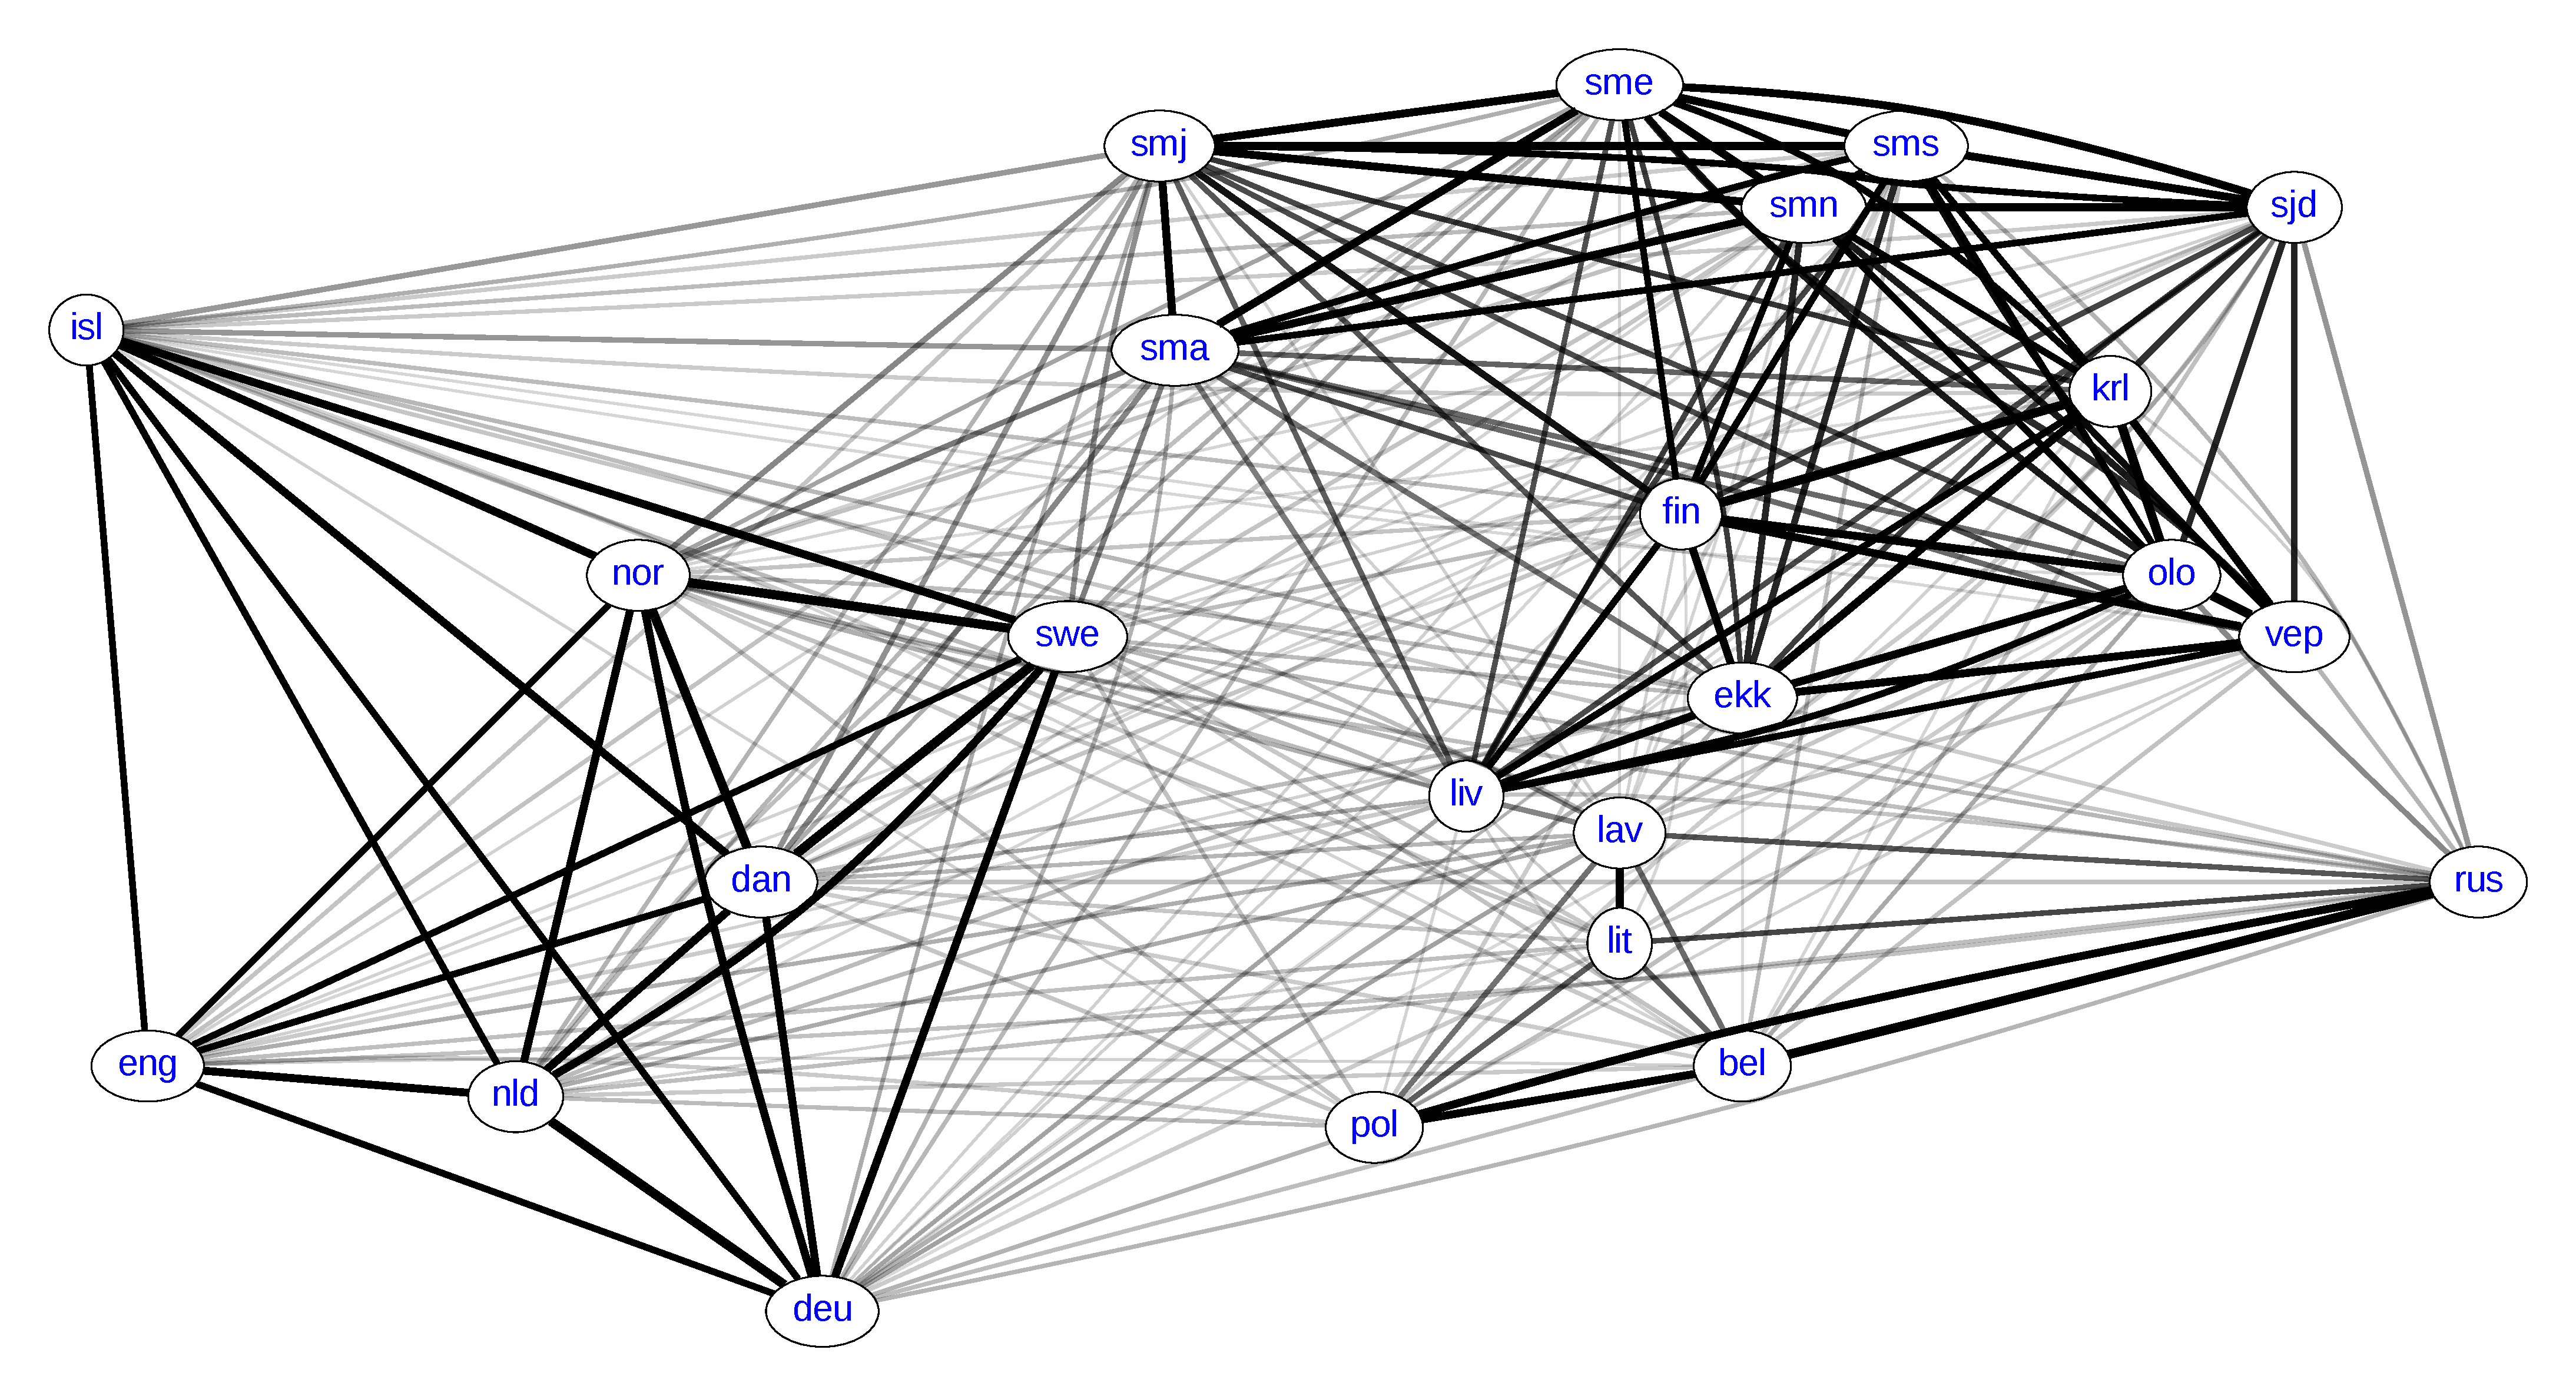
\includegraphics[width=\textwidth]{figures/cognacy-strength-baltic.pdf}
\caption{Visualization of inferred cognate overlap in the Baltic Sea data}
\label{baltic-cognacy}
\end{figure}

On the Indo-European side, southern Scandinavia is the homeland of the \ili{North Germanic languages} (\textit{swe}, \textit{dan}, \textit{nor}, \textit{isl}), which have evolved from the \ili{Old Norse} of the Viking Age, whose Western dialect developed into the West Scandinavian languages \ili{Icelandic} (\textit{isl}), \ili{Faroese}, and \ili{Norwegian} (\textit{nor}), whereas the Eastern dialect gave rise to \ili{Danish} (\textit{dan}) and \ili{Swedish} (\textit{swe}). The position of Norwegian in this genealogical tree is a little problematic, because Norwegian has a lot of dialectal variation, and two quite different written standards. The \ili{Nynorsk} standard can, with some justification, still be called a West Scandinavian language, whereas the \ili{Bokm\aa{}l} variant represented in NorthEuraLex is much more similar to the East Scandinavian languages. As another native language of the region of high historical significance, \ili{German} (\textit{deu}), which belongs to the West Germanic branch, is
also part of this case study. From a historical perspective, it would have made more sense to include \ili{Low German} instead of Standard High German, but no variant of Low German is featured in NorthEuraLex so far.

The only \ili{Slavic languages} with any relevance for the Baltic sea region are \ili{Polish} (\textit{pol}) as well as \ili{Russian} (\textit{rus}) and closely related \ili{Belarusian} (\textit{bel}). The Slavs originally settled a homeland somewhere in Eastern Poland or Western Ukraine, and began their rapid expansion in all directions as late as 500 AD \citep{kobylinski2005}. In later centuries, when Russian had become the state language of a great power with major strategic interests in the region, it started to exert a dominating influence on all languages on the eastern coast of the Baltic sea as well \citep{decsy1988}. \cite{smolicz_radzik_2004} summarize how during its short history, literary Belarusian has continually been remolded to be either lexically closer to Polish (\textit{pol} \arrowOA \textit{bel}) or to Russian (\textit{rus} \arrowOA \textit{bel}) depending on the political situation, and show that its present role, despite being the titular state language of Belarus, is in many ways more
similar to an endangered minority language.

The \ili{Baltic languages}, which show so much similarity with the Slavic languages that a single Balto-Slavic branch of Indo-European is generally assumed, once settled a large area north of the Slavs, but have since been gradually displaced by expanding Germans and Slavs, except for two surviving languages of the Eastern Baltic branch, \ili{Lithuanian} (\textit{lit}) and \ili{Latvian} (\textit{lav}), which are the national languages of the respective modern states. \ili{Old Prussian}, the ancient language of Prussia which became extinct through replacement with German in the 18th century, is the single relatively well attested Western Baltic language, but it cannot be included in NorthEuraLex because information on only a fraction of the relevant concepts is available.

According to \cite{viitso1998}, the \ili{Finnic languages} (\textit{fin}, \textit{krl}, \textit{olo}, \textit{vep}, \textit{ekk}, \textit{liv}) form an ancient dialect continuum reaching around the Gulf of Finland, where \ili{Finnish} (\textit{fin}) and Standard \ili{Estonian} (\textit{ekk}) became national languages during the 19th century, and others have survived as small minority languages of northwestern Russia, predominantly in the Republic of Karelia. Of these smaller languages, NorthEuraLex contains two written variants of \ili{Karelian} (\ili{North Karelian} \textit{krl} and \ili{Olonets Karelian} \textit{olo}), and the \ili{Veps} language (\textit{vep}). Moreover, NorthEuraLex contains data for the recently extinct \ili{Livonian} (\textit{liv}) of Latvia.

The \ili{Saami languages} (\textit{sma}, \textit{smj}, \textit{sme}, \textit{smn}, \textit{sms}, \textit{sjd}) form another ancient dialect continuum \citep{sammallahti1998} across northernmost Scandinavia, which is conventionally split into at least ten languages, six of which have standardized literary variants. Western Saami (\textit{sma}, \textit{smj}, \textit{sme}) consists of \ili{Southern Saami} (\textit{sma}), \ili{Lule Saami} (\textit{smj}), and \ili{Northern Saami} (\textit{sme}), which is by far the most thriving of the Saami languages, and is becoming a lingua franca for all Saami speakers due to its large number of speakers, the central position it takes in the dialect continuum, and its state-sponsored role as a media and academic language. The Eastern Saami languages (\ili{Inari Saami} \textit{smn} and \ili{Skolt Saami} \textit{sms} in Finland, as well as \ili{Kildin Saami} \textit{sjd} on the Kola peninsula) are all severely endangered, with only a few hundred speakers left for each of them.

As shown by \cite{aikio2006contacts}, already the Nordic Bronze Age culture before 500 BC appears to have had intensive trade contacts with Finnic tribes in the Baltics, and Saami tribes in Finland. During the early Middle Ages, when the Saami had settled Northern Scandinavia, and Southern Finland had been colonized by the Finns, these contacts intensified. After christianization, Swedish settlers started to colonize parts of Finland's coastal areas in the 12th century. The influx of settlers continued into the times of the Northern Crusades, as a result of which Western Finland became part of the Swedish state. \ili{Swedish} as the language of administration and education had a strong influence on the western dialects of \ili{Finnish}, which later became the basis for the written standard (\textit{swe} \arrowLA \textit{fin}). At the same time, Russian missionaries had started to spread the orthodox faith among the Finnic tribes of the east, which both influenced the later national borders between Swedish
Finland and Novgorod (and later Russia), and contributed to the concept of separate Finnish and Karelian nationalities. The lexical impact of \ili{Russian} on the \ili{Karelian} dialects was of a similar nature as that of Swedish on Finnish in the west (\textit{rus} \arrowLA \textit{krl, olo}). According to \cite{puura_ea_2013}, Russian influence on spoken \ili{Veps} has been quite strong as well due to near-complete bilingualism. In contrast, the recently published dictionaries such as \cite{zajceva2010} are quite purist, which means that only very few Russian loans are visible in the NorthEuraLex data for this language. This hints at a more general problem with representing minority languages in lexical databases. Due to purist attitudes, Russian loans, even if they are the first words that come to mind for certain concepts, will not be accepted as part of their language by dictionaries or native informants, even though the words given instead might already have fallen out of actual use.

\cite{zachrisson2008} provides an overview of later interactions between North Germanic peoples and the Saami. Since the late Middle Ages, when \ili{Saami languages} were still spoken much further to the south, the development of the centralized Scandinavian nation states, and accompanying christianization, has been causing the Saami population to assimilate, or migrate further to the north. For centuries, the language policy of the Scandinavian nation states was to ban the use of Saami languages at school and in public life \citep{corson1995}, which has led to intensive pressure of the North Germanic state languages\il{North Germanic languages} on the \ili{Western Saami languages} (\textit{swe} \arrowLA \textit{Western Saami}, \textit{nor} \arrowLA \textit{Western Saami}). The same pattern, along with its role as a trade language, has led to massive Finnish influence on \ili{Northern Saami} (\textit{fin} \arrowOA \textit{sme}), \ili{Inari Saami} (\textit{fin} \arrowOA \textit{smn}), and, chiefly after the
Skolts' resettlement during the aftermath of the Second World War \citep{feist2011}, on \ili{Skolt Saami} (\textit{fin} \arrowOA \textit{sms}). The \ili{Eastern Saami languages}, which were once spoken across Karelia, had previously been influenced \citep{sergejeva2000} by neighboring North Karelians (\textit{krl} \arrowOA \textit{Eastern Saami}), and then of course by the Russian state language (\textit{rus} \arrowLA \textit{sjd, sms}).

Some of the earliest language contacts in the region occurred between Finnic and Baltic tribes at a time when the Slavs had not yet expanded to the north. \cite{suhonen1988} lists a large number of ancient Baltic\il{Baltic languages} loans in the \ili{Finnic languages}, covering semantic fields such as basic tools and agriculture, many animal and plant names, and female kinship terms (\textit{Baltic \arrowLA Finnic}). While the frequency of Baltic loans is highest in \ili{Finnish}, \ili{Estonian}, and \ili{Olonets Karelian}, this effect, as Suhonen himself points out, might be simply due to the less well-developed lexicography in the smaller Finnic languages. Moreover, \cite{suhonen1973} counts more than 2,200 recent \ili{Latvian} loans in the \ili{Livonian} language (\textit{lav \arrowLA liv}), an interesting case of overwhelming influence of a written majority language on a barely written minority language, while the majority language is itself but a regional minority language in a much larger state.

In Estonia and Latvia, Hanse traders and especially the crusaders of the Teutonic Order, who founded their state in the Baltics in the 13th century, brought the \ili{German} language with them. As \cite{rot1988} demonstrates, German had an enormous impact on the cultural vocabulary of both the \ili{Estonian} language (\textit{deu} \arrowLA \textit{ekk}) and then still widespread \ili{Livonian} (\textit{deu} \arrowLA \textit{liv}). Some of these words were also borrowed into \ili{Latvian} (\textit{deu} \arrowOA \textit{lav}). Although both countries ended up protestant after the reformation, the early missionary activities by the orthodox church are still visible in the religious vocabularies of both languages, and further influence of the dominant language during Imperial \ili{Russian} and Soviet times has left traces (\textit{rus} \arrowLA \textit{ekk}, \textit{rus} \arrowOA \textit{lav}).

Further to the south, \ili{Lithuanian} was not influenced by German to the extent that the other languages of the Baltics were, due to a separate statehood tradition which aligned Lithuanians more closely with Poland than with their other neighbors. As \cite{senn1944} writes, 16th-century Lithuanian still showed quite a bit of influence of \ili{Polish} and \ili{German}, but most of these loans were removed from the language due to later purist attitudes, such that modern Lithuanian contains almost no borrowings in its basic vocabulary.

On the south coast of the Baltic sea, exchange between Germans and Slavs has led to some mutual influence, which has left the basic vocabulary largely untouched, however. Also, the more recent loans from German into Polish do not exceed a handful among the concepts covered by NorthEuraLex. The influence of German on its much more closely related northern neighbors has been more pronounced, with written German being a strong influence on the development of all three modern written standard languages of Scandinavia (\textit{deu} \arrowOA \textit{dan}, \textit{swe}, \textit{nor}), while Icelandic stayed untouched by these developments due to its isolation. During the centuries of Danish rule over Norway, the more widespread Bokm\aa{}l of the two competing written forms of Norwegian, was very much molded after the model of Danish on every level (\textit{dan} \arrowOA \textit{nor}), which is still visible in the fact that it now resembles its East Scandinavian neighbors much more (to the point of mutual intelligibility) than its West Scandinavian sister language Icelandic.

To summarize, \figref{baltic-goldstandard-phylo} visualizes the gold standard for phylogenetic lexical flow inference on the dataset. The proto-languages are located roughly at their reconstructed positions, with some modifications which had to be made for readability. Inheritance relationships are visualized with black arrows, bidirectional contact with light green lines (not in this case study), and unidirectional contacts are shown as dark green arrows. Sometimes, some arrows will deviate from the gold standard motivated in the text. In such cases, the deviating arrows will represent the closest equivalent to a relevant contact where one of the proto-languages was not present in the reduced tree.

\begin{figure}
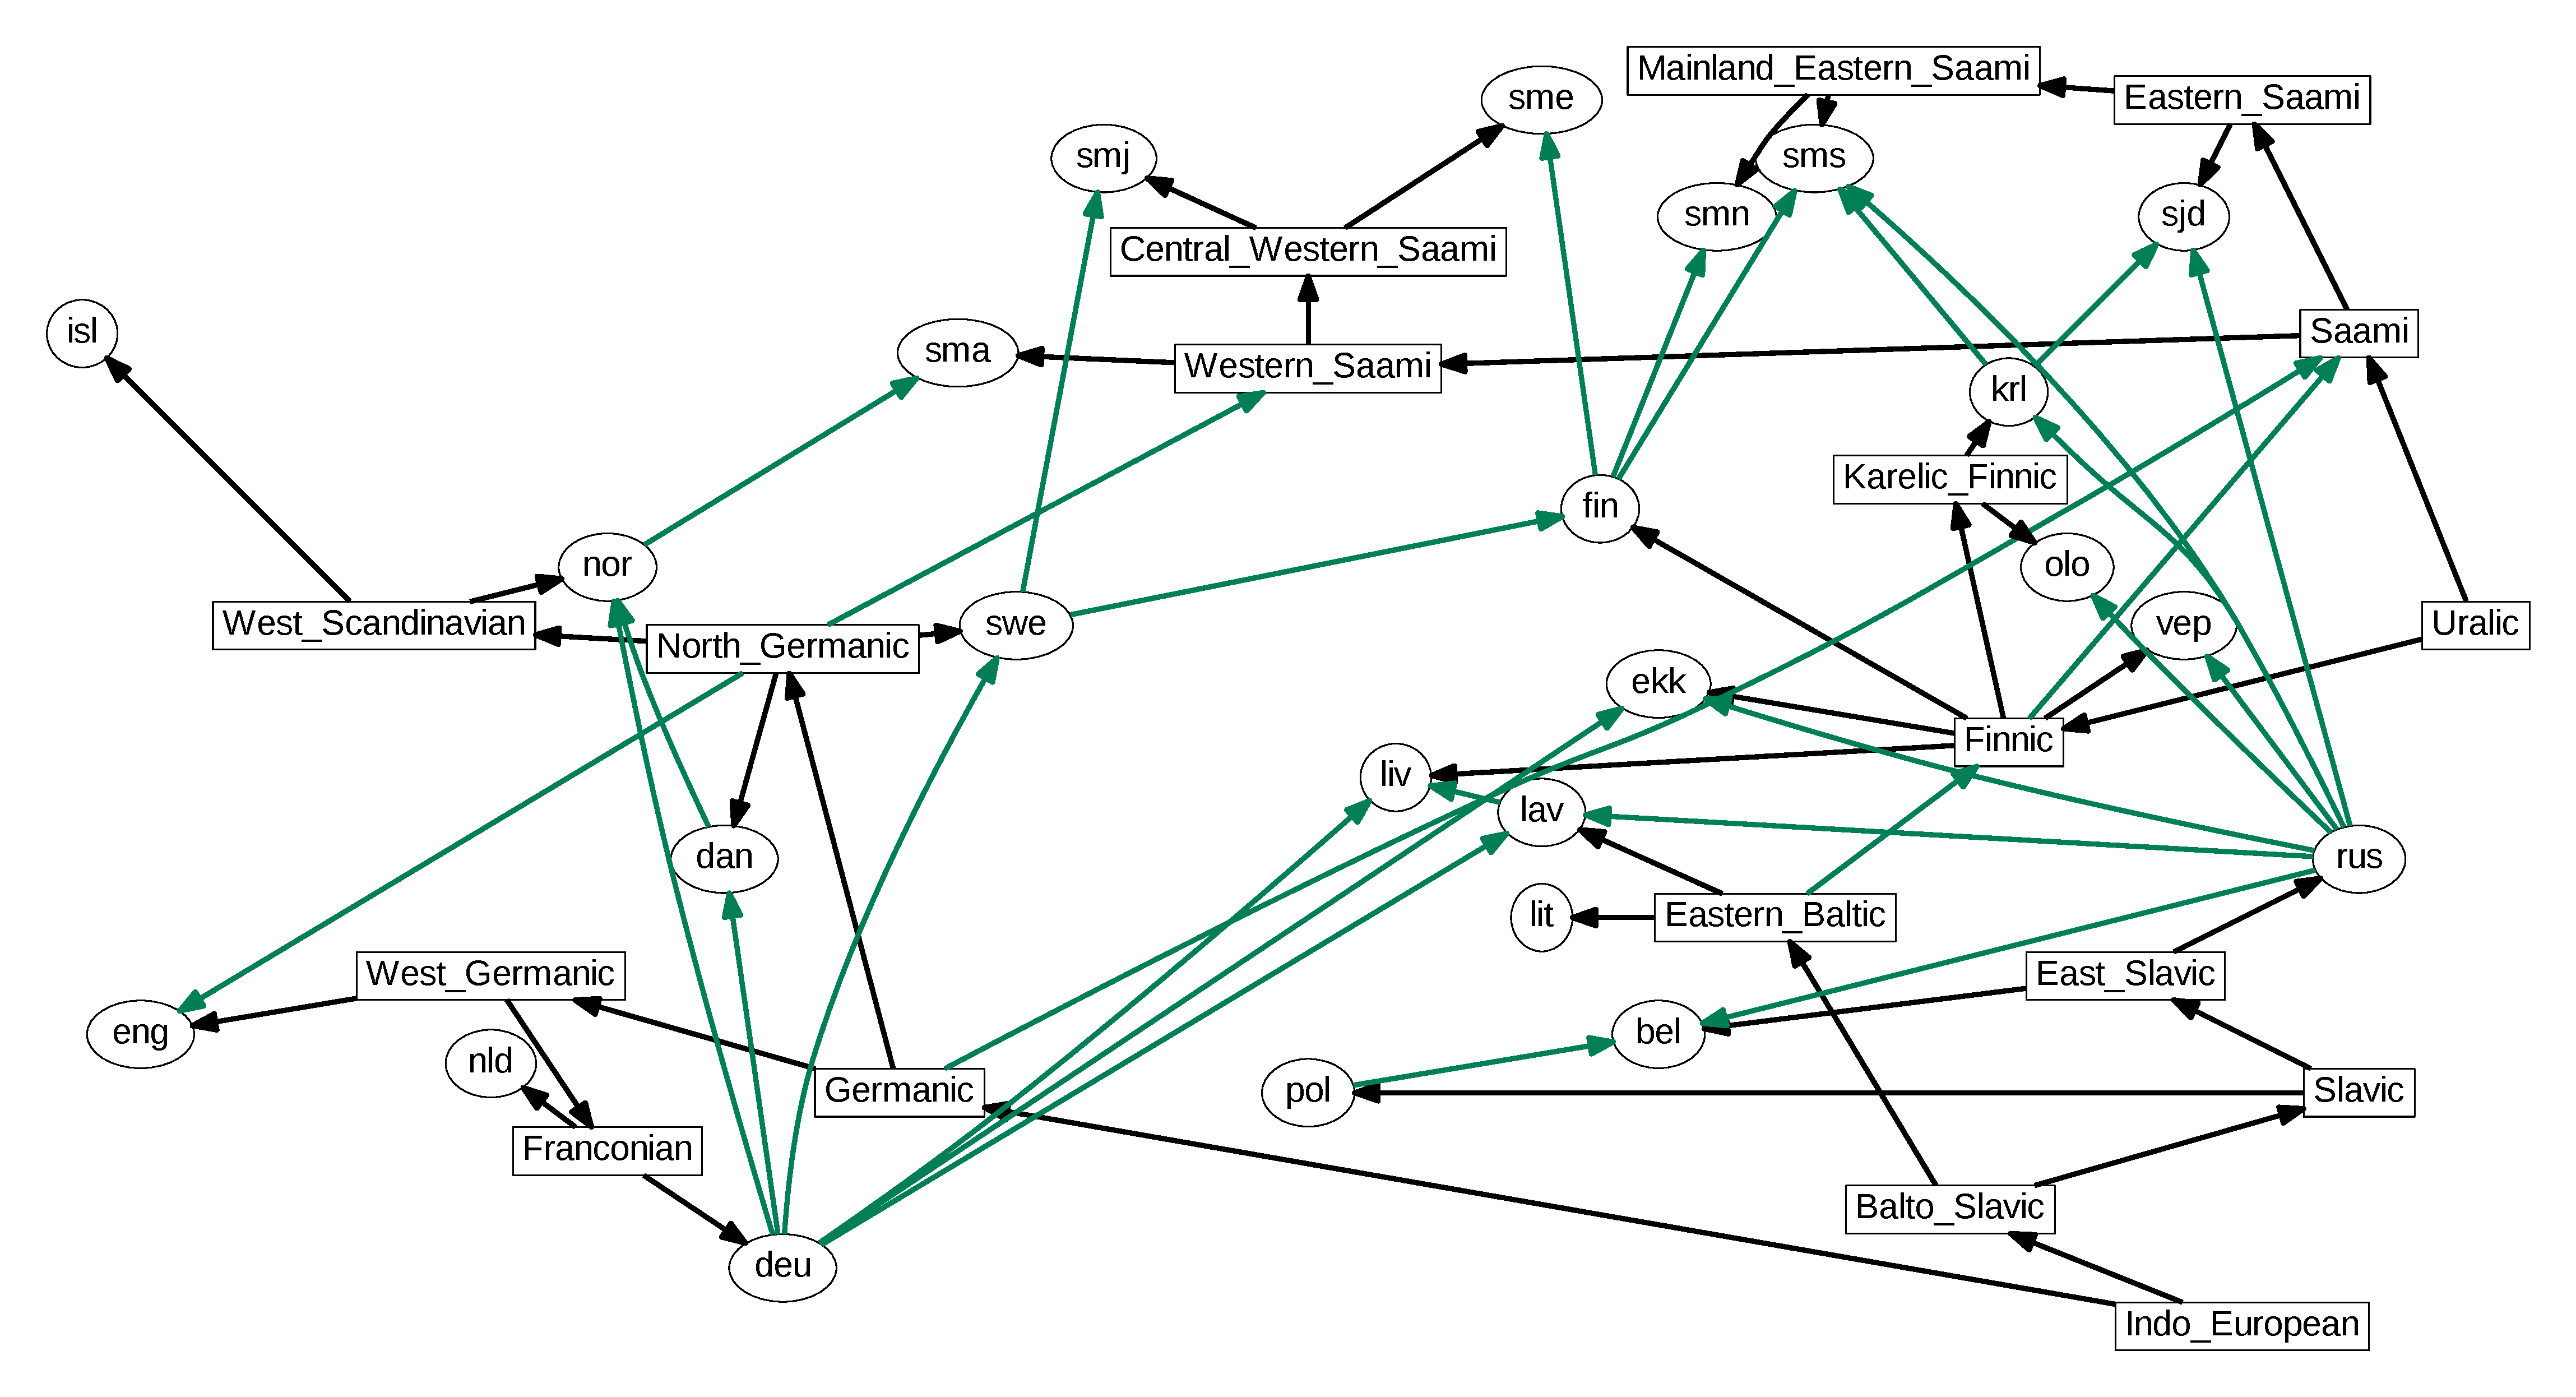
\includegraphics[width=\textwidth]{figures/goldstandard-phylo-baltic.pdf}
\caption{Gold standard for phylogenetic flow on Baltic Sea data}
\label{baltic-goldstandard-phylo}
\end{figure}

\subsection{Case study 2: Uralic and contact languages}
The second case study expands our horizon eastwards, to the point that it includes the Uralic languages with all their contact neighbors. This leads to a focus on European Russia, Scandinavia, and Western Siberia. Hungarian as a geographic outlier requires us to additionally include some further languages of Central and Eastern Europe, whereas the historical contacts of Uralic languages in Central Russia with Turkic neighbors leads us to also include some of the northern outliers of that family into the sample. We end up with a contact inference problem for a region stretching across 6,000 kilometers from west to east, and more than 3,000 kilometers from north to south, all of which is covered reasonably well by NorthEuraLex.

The Uralic language family\il{Uralic languages} consists of about 36 living languages (24 of which are covered by NorthEuraLex), which fall into nine firmly established branches. From west to east, these are Finnic, Saamic, Mordvinic, Mari, Permian, Hungarian, Mansi, Khanty, and Samoyedic. The highly divergent \ili{Samoyedic languages} are traditionally seen as forming the primary split within Uralic, with all the other branches being grouped together as Finno-Ugric\il{Finno-Ugric languages}. However, previously undetected cognates between Samoyedic languages and Eastern branches of Finno-Ugric have recently been discovered \citep{aikio2002,aikio2006etym}, which has considerably increased the number of reconstructable roots of Proto-Uralic, and contributed to a tendency to not necessarily assume this primary split to hold any longer. Moreover, a recent reanalysis of vowel correspondences \citep{hakkinen2007} has yielded some evidence that the primary split might have been between Finno-Permic\il{Finno-Permic languages} comprising the five western branches, and Ugro-Samoyedic on the other side, which then split into the four eastern branches. For the purposes of this work, the question of the internal structure of Uralic can be considered as open, and we will simply assume a comb-like structure formed by all the safely established branches.

The western branches Finnic and Saami were already described as part of the linguistic background for the first case study. Considering their relationship with the rest of Uralic, the Saami languages share so much lexical material with Finnic that these two branches have traditionally tended to be seen as forming a single Finno-Saamic\il{Finno-Saamic languages} phylogenetic unit. \cite{aikio2012} summarizes arguments for and against a closer affinity. The main problem is that the two branches do not show enough shared innovations in phonology to exclude ancient contacts as an explanation for their considerable lexical overlap. However, there still are some shared morphological innovations which are difficult to explain by contact alone.

The \ili{Mordvinic languages} (\textit{myv}, \textit{mdf}) and the \ili{Mari languages} (\textit{mhr}, \textit{mrj}), both of which could also be treated as dialect continua with two written standards each, have often been grouped together as the Volga-Fennic languages, but after a reassessment by \cite{bereczki1988}, this is now generally seen as a purely geographic grouping. Instead, as \cite{gruenthal2007} shows, if Mordvinic is considered part of a larger phylogenetic unit, it tends to be grouped together with Finnic and Saamic on lexical grounds.

Further to the east, the \ili{Permian languages} (\textit{kpv}, \textit{koi}, \textit{udm}) form the last branch of what some authors accept as the Finno-Permic branch of the Finno-Ugric languages. The Permian languages are closely related, with \ili{Udmurt} (\textit{udm}) in the Republic of Udmurtia being the most divergent. With more than 300,000 speakers, Udmurt is among the more viable minority languages of Russia. The other branch of Permic is formed by the highly divergent dialects of the Komi language, two of which are written languages. The 150,000 speakers of \ili{Komi-Zyrian} (\textit{kpv}) are distributed across a wide area in the northeastern part of European Russia. It is also one of the official languages in the Komi Republic, a very large territory covering much of the area west of the northern half of the Ural mountains. \ili{Komi-Permyak} (\textit{koi}), with little over 100,000 speakers, is the written standard for the Komi-Permyak Okrug in the Perm Krai, the Russian region south of the Komi Republic. The region around the Kama river where Udmurt and Komi-Permyak are spoken today is currently considered the most likely candidate for a Uralic urheimat \citep{hakkinen2009}, though alternative theories about a Siberian urheimat remain justifiable if one still assumes Samoyedic to form the primary split. Previous theories placing the homeland farther into Europe were based on archeological continuity arguments, and are now considered obsolete due to their lack of reliability \citep{hakkinen2006}.

In Western Siberia, the dialects of \ili{Khanty} (\textit{kca}) and \ili{Mansi} (\textit{mns}) have traditionally been grouped together as the \ili{Ob-Ugric languages}, but the close affinity is not accompanied by any shared innovations, and is therefore now seen by many uralists, like \cite{salminen2002}, as more likely due to intensive lexical contact (\textit{mns} \arrowOA \textit{kca} and \textit{kca} \arrowOA \textit{mns}). The \ili{Mansi} dialects are spoken by less than 1,000 people in the western parts of the Khanty-Mansi Autonomous Okrug, which covers a large part of the middle Ob and its tributaries east of the central Urals. \ili{Khanty} dialects are still spoken by almost 10,000 speakers in the eastern parts of the okrug, as well as neighboring areas to the north and east. \ili{Hungarian} (\textit{hun}) has been so much reshaped by its intensive contacts with other language families during the century-long migration of its speakers, that it now appears to form a branch of its own, although many
isoglosses with the Ob-Ugric languages, particulary Mansi, do exist (such as the intensive use of verbal particles, highly unusual of Uralic), causing it to be placed next to the Ob-Ugric languages in all proposals of larger subunits. Lexically, the overlap with Khanty is stronger than that with Mansi, which is generally attributed to mutual contact (\textit{kca} \arrowOA \textit{hun} and \textit{hun} \arrowOA \textit{kca}).

Finally, the four \isi{Samoyedic languages} (\textit{yrk}, \textit{enf}, \textit{sel}, \textit{nio}) form the easternmost branch of Uralic. The internal structure of this branch is not very clear. On lexical grounds, the southernmost surviving language Selkup (\textit{sel}) is clearly divergent from its northern relatives, but according to many other criteria, the Nganasan language (\textit{nio}) on the remote Taimyr peninsula is clearly the outlier. Perhaps due to its isolation, Nganasan is a very conservative language which shares some striking features (consonant gradation, vowel harmony) with the westernmost branch Finnic, hinting that these traits may have been present already at a very early stage of Uralic. By far the most viable of the Samoyedic languages is Nenets (\textit{yrk}), whose Tundra variant with more than 20,000 speakers is spoken in the far north on both sides of the Ural mountains. Closely related Enets, whose forest variant (\textit{enf}) is represented in NorthEuraLex, was once spoken along
the entire lower Yenisei, but has been brought close to extinction under pressure of both Tundra Nenets and Russian. Selkup is still spoken by about 1,000 people in the region between Ob and Yenisei, and is the last surviving Southern Samoyedic language, which once also included the now extinct Kamassian and Mator languages of the Sayan mountains west of Lake Baikal.

While the contacts between Western Uralic and Germanic or Baltic languages in the Baltic sea region were already described in the preceding section, the complex contact history of \isi{Hungarian} (or Magyar) warrants some more detailed remarks. During their long migration from the Ural region (where the closest relatives Khanty and Mansi still reside) to central Europe, a process which most probably took about 2,000 years, \ili{Hungarian} first had intensive contact with the \ili{Permian languages} (\textit{hun} \arrowOA {Permian} or \textit{Permian} \arrowOA {hun}). Leaving the area of Uralic speakers on their way to the southwest, Hungarians next encountered and were influenced by Iranian\il{Iranian languages} tribes (\textit{Iranian \arrowLA hun}), and later ended up under G\"oktürk rule on the Black Sea, where Western \ili{Turkic languages} became the source of a lot of cultural vocabulary (\textit{Turkic \arrowLA hun}). After the collapse of the Khazar empire, the Hungarians then undertook their final migration westward, conquering and settling in the Carpathian Basin at the end of the ninth century. Here, they acquired further strata of loans from both West Slavic\il{West Slavic languages} and South Slavic\il{South Slavic languages} (\textit{West Slavic, South Slavic \arrowLA hun}), especially in the semantic fields of agriculture and household items. \ili{German} influence is especially visible in the fields of military and engineering, whereas \ili{Latin} provided the words for many religious and philosophical concepts. While the rapidly expanding Kingdom of Hungary had Latin as its official language well into the 19th century, limiting the influence of Hungarian on the Slavic minorities, Hungarian language policy during the late stages of the Austro-Hungarian empire developed a strong tendency towards Magyarization. This led to Hungarian influence especially on \ili{Croatian} and \ili{Slovak}, although this is barely visible in the basic vocabulary. The same is true for \ili{Turkish} influence during the period of Ottoman rule in the 16th and 17th centuries.

The other major historical influence on Uralic languages is caused by the direct neighborhood of the Volga-Fennic and southern Permian languages with the Turkic languages \ili{Chuvash} (\textit{chv}), \ili{Tatar} (\textit{tat}), and \ili{Bashkir} (\textit{bak}). In the case of the \ili{Mari languages}, the influences of neighboring Chuvash (\textit{chv \arrowLA Mari}) and Tatar (\textit{tat \arrowLA Mari}) is the strongest. Among \ili{Permian languages}, \ili{Udmurt} has become most influenced by its Turkic southern neighbors Tatar (\textit{tat \arrowLA udm}) and Bashkir (\textit{bak \arrowLA udm}). These contacts, including layers of loans which have not had much influence on the basic vocabulary, are described extensively by \cite{rona-tas1988}.

After the initial splits, there has been some limited contact between neighboring branches of Uralic. According to \cite{hausenberg1998}, Komi merchants caused \ili{Komi-Zyrian} to become an influential trade language of the north, with some influence on \ili{Nenets} (\textit{kpv} \arrowOA \textit{yrk}) and \ili{Mansi} (\textit{kpv} \arrowOA \textit{mns}), which is however only barely visible in the basic vocabulary of these languages. In the east, \ili{Khanty} and \ili{Selkup} have interacted quite intensively (\textit{kca} \arrowOA \textit{sel}), and \ili{Enets} was heavily influenced through mixed marriages with the closely related and much more vital Nenets community (\textit{yrk} \arrowOA \textit{enf}) before its few remaining speakers started shifting towards \ili{Russian} \citep{siegl2013}.

The pervasive development in all the Uralic minority languages, however, is a shift towards \ili{Russian} as the language of school and the workplace. While some of these languages still have hundreds of thousands of speakers, in all cases the speaker communities are dominated by the old people in rural areas, whereas city life as well as mass culture and all modern economic activity takes place exclusively in Russian. This very strong tendency puts the future of all the Uralic minority languages very much into question, even more so as the current political climate tends to be hostile to any activities which can be interpreted as fostering separatist tendencies within Russia \citep{taagepera2013}.

But Russian influence does of course reach back much farther than the introduction of a comprehensive school system by the Soviets. Russian influence on the lexicon is observable in all minority languages, but some languages (\ili{Kildin Saami}, \ili{Erzya}, \ili{Hill Mari}, \ili{Udmurt}, \ili{Komi}) show more Russian influence even in basic vocabulary than others which tend to be more purist at least in their written variants (\ili{Moksha}, \ili{Meadow Mari}). The following contacts are reflected so strongly in the basic vocabulary that they were added to the gold standard: \textit{rus} \arrowLA \textit{olo, vep, sjd, sms, myv, mrj, udm, koi, kpv, kca, mns, yrk, sel, enf, nio}.

Among the languages which are included in this case study chiefly by virtue of having been in contact with \ili{Hungarian}, \ili{Romanian} is a Romance language whose lexicon was heavily influenced by surrounding \ili{Slavic languages} (\textit{Slavic} \arrowOA \textit{ron}). According to \cite{schulte2009}, there are also traces of \ili{German} (\textit{deu} \arrowOA \textit{ron}) and Hungarian (\textit{hun} \arrowLA \textit{ron}) loans in the basic vocabulary. Outside the scope of this case study, Romanian also contains a layer of ancient loans from \ili{Albanian} or a closely related language (\textit{sqi} \arrowOA \textit{ron}), many loanwords from written \ili{Latin} (\textit{lat} \arrowOA \textit{ron}) as well as some from \ili{Greek} (\textit{ell} \arrowOA \textit{ron}). A substantial number of later loans came from \ili{Turkish} (\textit{tur} \arrowLA \textit{ron}), and the words for many concepts of modern life were borrowed from \ili{French} (\textit{fra} \arrowOA \textit{ron}).

\figref{uralic-cognacy} visualizes the cognacy overlaps between the \ili{Uralic languages} and their neighbors. The rather chaotic picture already indicates that this case study is more of a challenge for lexical flow detection than the Baltic Sea study. The highest overlaps cluster the Western Uralic languages (Finnic and Saami) together. Also, the Germanic\il{Germanic languages} and \ili{Slavic languages}, the two Baltic languages as well as the four \ili{Turkic languages} clearly appear as clusters. The central and eastern branches of Uralic are clearly least distinctive, mirroring the unclear second-level structure of the family. \ili{Hungarian} has overlaps of medium strength with many Uralic languages as well as Slavic neighbors, making it a major challenge to detect its affinity with the \ili{Ob-Ugric languages}.

\begin{sidewaysfigure}
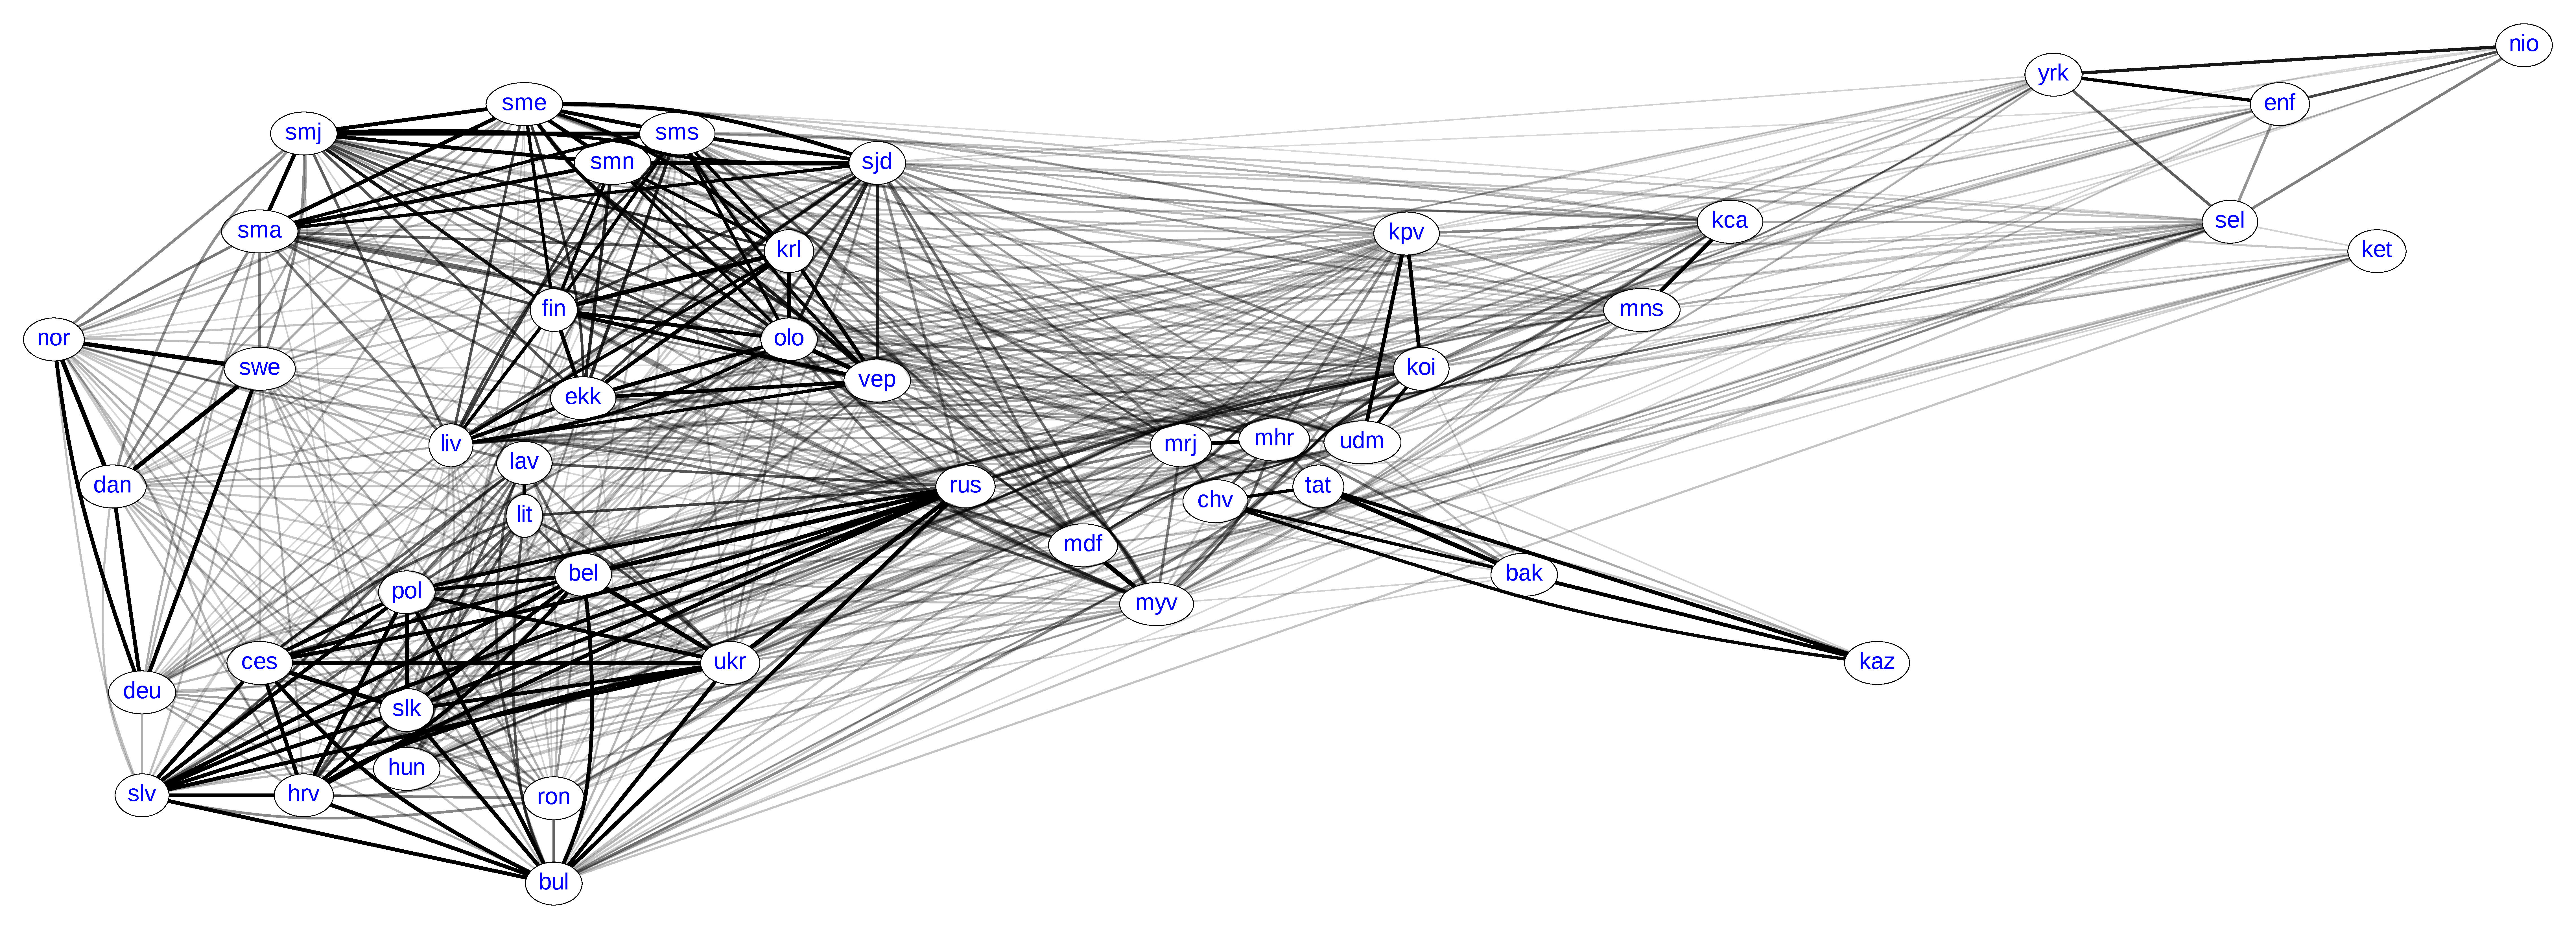
\includegraphics[width=\textwidth]{figures/cognacy-strength-uralic.pdf}
\caption{Visualization of inferred cognate overlap in the Uralic data}
\label{uralic-cognacy}
\end{sidewaysfigure}

\figref{uralic-goldstandard-phylo} visualizes the ideal result of phylogenetic flow inference. Note that some of the connections of \ili{Hungarian} are light green lines, indicating that the direction of influence is unclear, which makes an undirected arc in an automatically inferred network just as acceptable as an arrow in either direction.

\begin{sidewaysfigure}
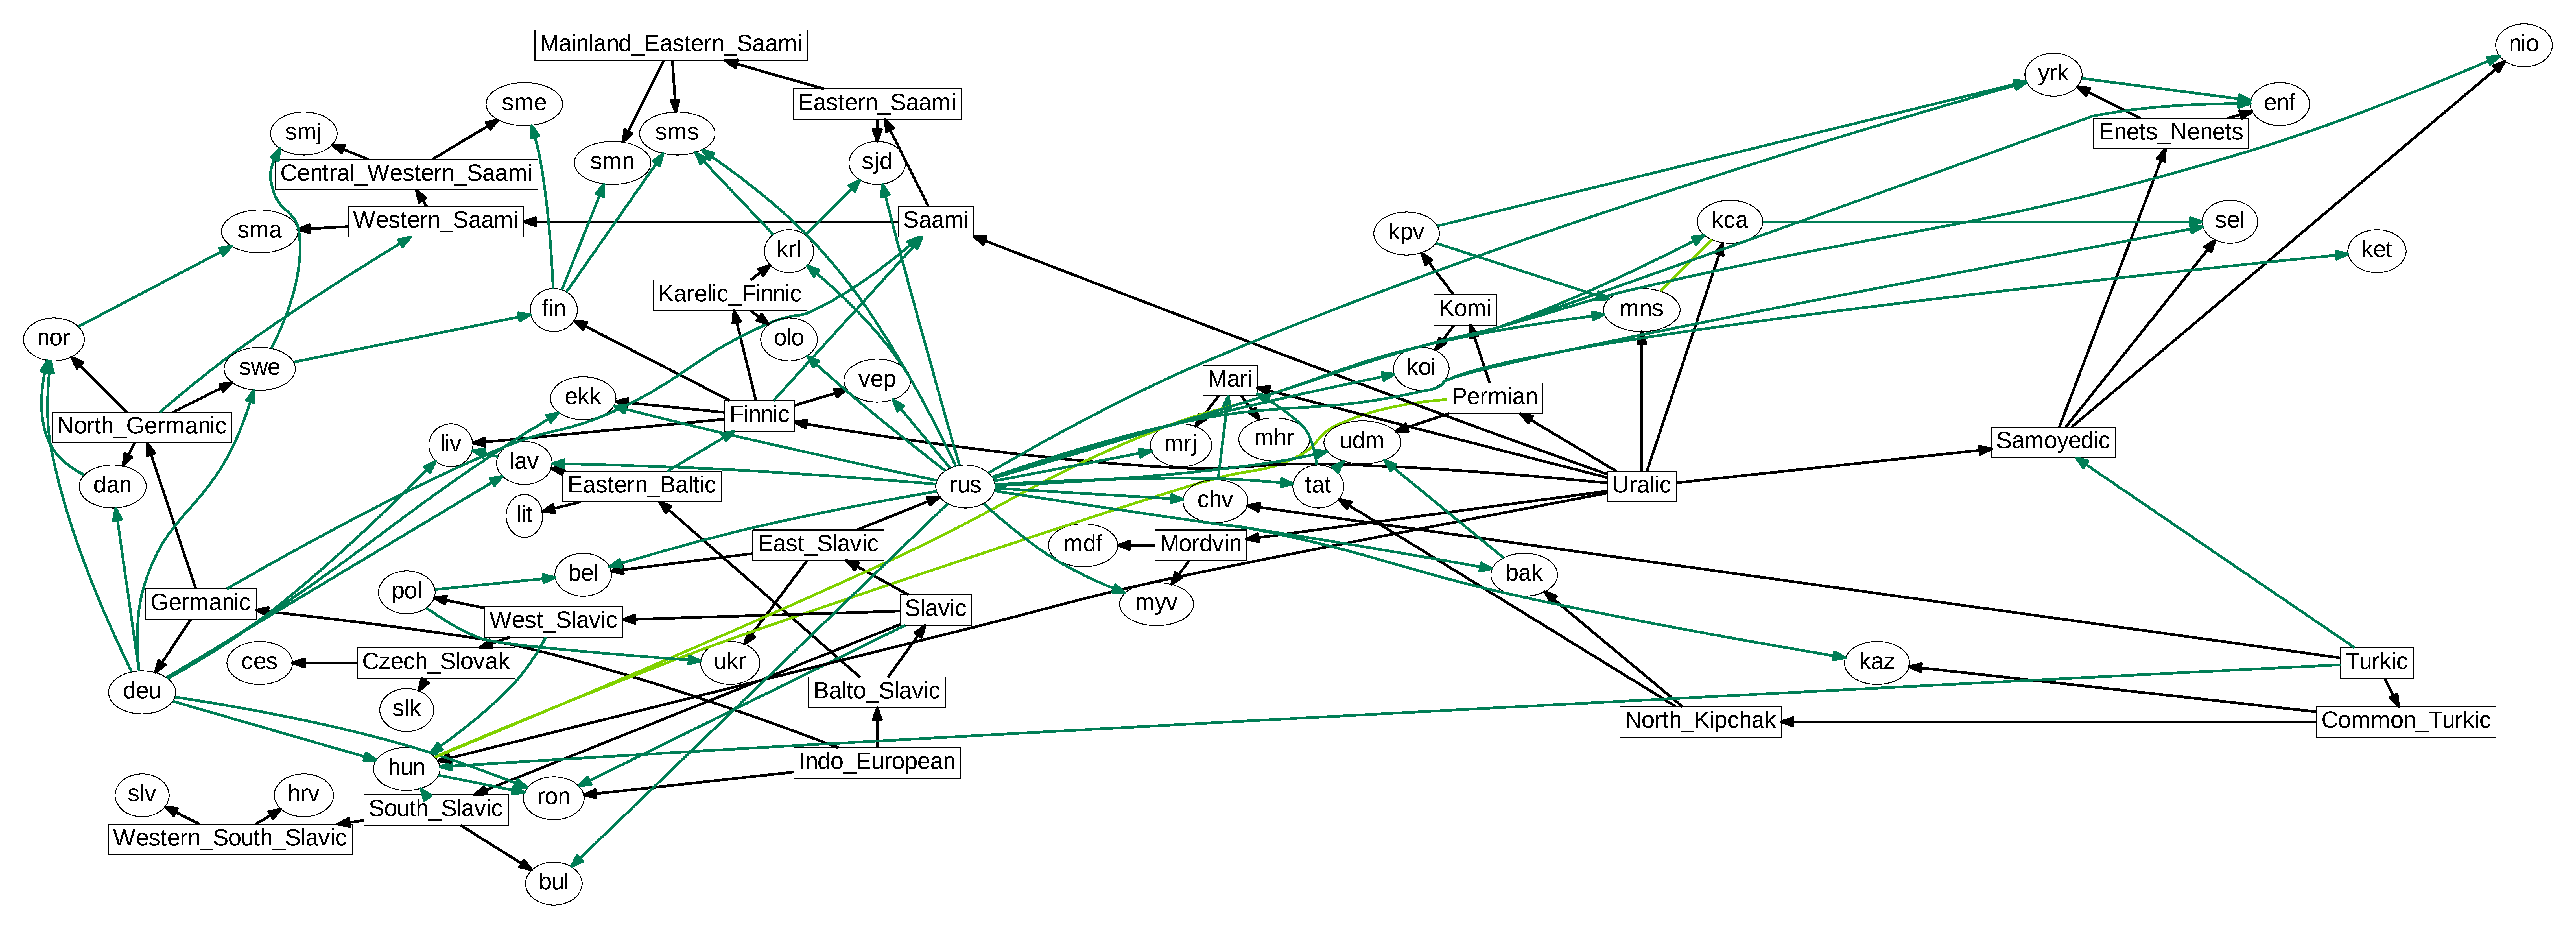
\includegraphics[width=\textwidth]{figures/goldstandard-phylo-uralic.pdf}
\caption{Gold standard for phylogenetic flow on Uralic data}
\label{uralic-goldstandard-phylo}
\end{sidewaysfigure}

\subsection{Case study 3: The linguistic landscape of Siberia}
The next case study deals with inferring contacts between the languages of Si\-be\-ria. Si\-be\-ria is a sparsely populated region where many ancient language families were able to survive until today, although all of the oldest languages have become small minority languages on the verge of disappearing. The number of language families in this test set is much larger than in the previous ones, and the high number of isolates generates additional challenges to lexical flow inference.

The dominant influence of the colonial language \ili{Russian} is of course visible in every minority language of Siberia. Some languages show less influence in the basic vocabulary than others, however. For instance, \ili{Itelmen} has borrowed extensively from Russian even in its basic vocabulary, whereas pressure on related \ili{Chukchi} was noticeably lower, most likely due to much later colonization (early 18th vs. early 20th century). While Russian has borrowed some words from \ili{Turkic languages}, this has not left measurable traces in the basic vocabulary, and borrowings from other Siberian languages only occur in specialized areas of local significance, such as reindeer herding, tent styles, and animal and plant names.

In western Siberia, the eastern branches of Uralic\il{Uralic languages} (\textit{mns, kca, sel, yrk, enf, nio}) have interacted with each other as well as Siberian languages to varying degrees. The influences of Khanty on Selkup (\textit{kca} \arrowOA \textit{sel}) and of Nenets on Enets (\textit{yrk} \arrowOA \textit{enf}) were already discussed, as were the western contacts of the Ket language. Concerning influences on Uralic from the east, Samoyedic\il{Samoyedic languages} has borrowed a few dozen words from Early Turkic\il{Turkic languages} (\textit{Turkic \arrowLA Samoyedic}), which are summarized by \cite{dybo2007}. Also, \cite{anikin_helimski_2007} list substantial numbers of loans from Tungusic\il{Tungusic languages} into Samoyedic (\textit{Tungusic} \arrowLA \textit{Samoyedic}).

All three language families (Turkic, Mongolic, and Tungusic) which are subsumed as Core Altaic\il{Altaic languages} by advocates of a deep relationship, play major roles in the linguistic landscape of Siberia. While the exact relationship between these three well-established families (whose typological similarities are indeed quite striking) is an eternal bone of contention, it is clear that even if there were no ancestral relationship, the three proto-languages must have been in very intensive and long-lasting contact with each other. During recorded history, the \ili{Turkic languages} have formed the westernmost of the three families (starting out in the Altai region), the \ili{Mongolic languages} have been in the center (Mongolia and adjacent areas), and the Tungusic\il{Tungusic languages} tribes originally settled in the east (Manchuria). The contemporary distribution pattern still shows this general tendency, but has been complicated by many migrations of these highly mobile nomadic peoples. For
instance, the westernmost Mongolic language \ili{Kalmyk} (\textit{xal}) is spoken in Kalmykia, a republic in European Russia, whereas the easternmost Turkic language \ili{Sakha} (\textit{sah}) is spoken in the Sakha republic (also called Yakutia) which covers a large part of Eastern Siberia. Tungusic peoples have spread throughout Siberia, with the westernmost speakers of \ili{Evenki} (\textit{evn}) neighboring the Kets\il{Ket} on the Yenisei, and the \ili{Manchu} (\textit{mnc}) in the south at one point conquering China and becoming the ruling elite of Qing, the last imperial dynasty of China.

\ili{Turkic languages} (\textit{tur}, \textit{azj}, \textit{tat}, \textit{bak}, \textit{kaz}, \textit{uzn}, \textit{sah}, \textit{chv}) are present throughout Russia, the Caucasus, Central Asia, Northern Iran, and Turkey. The following summary is based on the handbook of Turkic languages edited by \cite{johanson_csato_1998}, with some additional information from \cite{menges1995}. In genealogical terms, the Oghur subbranch\il{Oghur Turkic languages}, to which the \ili{Chuvash} language (\textit{chv}) of European Russia belongs, is a clear outlier, with at least 2,000 years of separate development, which puts the date of the latest stage of Proto-Turkic at about 500 BC. The Chuvash language is closely related to the extinct languages of the Bulgars and Khazars, and some scholars consider it likely that the \ili{Hunnic} language was Oghur Turkic as well.

The rest of Turkic, also called \ili{Common Turkic}, forms a much closer genealogical unit,
which probably still formed a single dialect continuum in 550 AD, when the Turkic expansion set in. This is also the date of the first written records in a Turkic language, the Orkhon inscriptions of the G\"oktürk khaganate. During the Turkic expansion in the 6th-11th centuries, Common Turkic separated into five branches, four of which are represented in NorthEuraLex.

The major \ili{Oghuz Turkic languages} are \ili{Turkish} (\textit{tur}), \ili{Azeri} or Azerbaijani (\textit{azj}), and \ili{Turkmen}. The Oghuz tribes arrived in Central Asia during the 8th century, formed a new warrior elite governing older Iranian states, and then started to spread to the southwest in the 11th century, founding the Seljuk Empire and invading Anatolia, where they later formed the Ottoman Empire and modern Turkey.

The Kipchak tribes\il{Kipchak Turkic languages} spread to the northwest, their farthest outliers in the Ural region mixing with the local population and separating into \ili{Bashkir} (\textit{bak}) and \ili{Tatar} (\textit{tat}), whose contacts we already discussed when covering Uralic and its neighbors. Most Turkic languages of the North Caucasus belong to the Cuman branch of Kipchak, others to the Nogai branch, which also includes the \ili{Kazakh} (\textit{kaz}) language. Finally, \ili{Kyrgyz} and some related smaller languages form another branch of Kipchak.

The Karluk tribes\il{Karluk Turkic languages} migrated to the southeast, came into intensive contact with Islam, and played a big role in the politics of China, before becoming the ruling class of the Timurid empire. The Karluks later gave rise to the modern \ili{Uzbek} (\textit{uzn}) and \ili{Uyghur} ethnicities.

The final direction, the northeast, led some Turkic tribes into Siberia\il{Siberian Turkic languages}, where most (such as the Tuvans and Chulyms) stayed near the Altai mountains, whereas one tribe migrated far to the north and became the Sakha or Yakuts, now the titular nation of the Russian federal subject which is largest in area, the Sakha Republic, which covers more than 3 million square kilometers, and where the \ili{Sakha} language (\textit{sah}) is still spoken by 400,000 people, about 40\% of the population.

The final branch of Common Turkic, Arghu\il{Arghu Turkic languages}, only consists of \ili{Khaladj}, a minority language of 40,000 speakers in central Iran, which lets it fall outside the scope of a comprehensive lexical database of Northern Eurasia.

Only two of the Turkic languages in NorthEuraLex, \ili{Kazakh} and Sakha, are relevant for the Siberian case study. Spread across the steppe zone directly to the south of Western Siberia, the Kazakhs were in intensive contact with Mongolian tribes, and borrowed many words for military and administrative terms from them (\textit{Mongolic} \arrowLA \textit{kaz}). \ili{Sakha} (\textit{sah}) is the only Siberian Turkic language currently represented in NorthEuraLex, but by far the one which has had most influence on the linguistic history of Siberia. Sakha contains some lexical material borrowed from its Mongolic\il{Mongolic languages} southern neighbors (\textit{bua}, \textit{xal} \arrowLA \textit{sah}), whereas a lot of the vocabulary of modern life was taken over from \ili{Russian} (\textit{rus} \arrowLA \textit{sah}).

The \ili{Mongolic languages} (\textit{khk}, \textit{bua}, \textit{xal}) are concentrated in Mongolia and neighboring regions of Russia and China. A very comprehensive overview of the family is given by \cite{janhunen2003}, which is also my main source about Mongolic languages. As a language family, the time depth of Mongolic is not very high, as all the living and attested languages are descended from dialects of \ili{Middle Mongol}, the language of the Mongol Empire in the 13th century. The most divergent Mongolic language, the probably now extinct \ili{Moghol} language of Afghanistan, is actually a remnant of one of Genghis Khan's armies which was stationed there during those times. The other outlier is the \ili{Daur} language of Inner Mongolia and neighboring provinces of China, which is already very close (50\% lexical overlap) to \ili{Khalkha Mongolian}. The remainder of the language family is split into two dialect continua. Southern Mongolic contains several minority languages of Northern China, some of them (\ili{Mongguor}, \ili{Dongxiang}) with hundreds of thousands of speakers, whereas the larger dialect cluster, Central Mongolic, which covers the northern half of the language family's area, subsumes about 80\% of all speakers of Mongolic languages. Since documentation of all smaller Mongolic languages exists mostly in Chinese and is difficult to come by, NorthEuraLex currently only contains three variants of Central Mongolian, with very different and interesting contact histories.

\ili{Khalkha Mongolian}\il{Mongolian} (\textit{khk}), the national language of the Republic of Mongolia, is by far the most stable of all Mongolic languages, partly at the cost of other Central Mongolian languages which only count as dialects of the national language. While being rather purist in recent times, Khalkha Mongolian has small layers of loanwords from \ili{Old Turkic} (\textit{Turkic} \arrowLA \textit{khk}), \ili{Sanskrit}, \ili{Persian}, \ili{Arabic}, Tungusic, and Chinese, most of which do not involve the most basic vocabulary, and a large layer of recent \ili{Russian} loans (\textit{rus} \arrowLA \textit{khk}) for scientific and technical vocabulary. Dialects subsumed under the name \ili{Buryat} (\textit{bua}) are spoken in Southern Siberia, Eastern Mongolia, and adjacent areas of China. The variant included in NorthEuraLex is based on Russian sources, and therefore includes many loanwords from Russian (\textit{rus} \arrowLA \textit{bua}). The Buryats, the most populous indigenous nation of Siberia at the beginning of Russian conquest, have exerted considerable cultural influence on many of the neighboring peoples, especially \ili{Sakha} and the \ili{Tungusic languages}. \ili{Kalmyk} (\textit{xal}) is a written variant of \ili{Oirat}, a group of Mongolic dialects of limited mutual intelligibility with Khalkha whose 360,000 speakers are spread throughout the westernmost parts of Mongolia, Xinjiang, Kyrgyzstan, and Kalmykia on the lower Volga. During their expansion, the Oirats often formed federations with Kipchak\il{Kipchak Turkic languages} tribes, from whom they borrowed quite a bit of cultural vocabulary (\textit{Kipchak} \arrowLA \textit{xal}). The remaining Oirat communities seem to be in the process of losing their ancestral language, and even the official language of Kalmykia, with some 80,000 speakers left, is only spoken fluently by the elderly, ever since the transmission of Kalmyk culture to the younger generations was interrupted by Stalin's deportations, which led to the demise of a substantial part of the Kalmyk population, and left heavy traces on their language (\textit{rus} \arrowLA \textit{xal}).

The \ili{Tungusic languages} (\textit{evn}, \textit{gld}, \textit{mnc}), though covering a very large geographical area, are thinly dispersed and under threat. A compact overview of the Tungusic languages and their current situation is given by \cite{janhunen2005}. \ili{Xibo}, the largest surviving Tungusic language by number of speakers, and one of only two languages which are still learnt by children, is spoken by the descendants of a single tribe which was deployed to the border by the Qing government. Due to a lack of accessible resources on Xibo, the closely related and well-documented \ili{Manchu} language (\textit{mnc}), the national language of the Qing dynasty, which now only has a handful of elderly speakers left, was chosen to represent this branch of Tungusic. The Manchu of the written sources contains many loanwords from Chinese (\textit{cmn \arrowLA mnc}) and Mongolian (\textit{khk \arrowLA mnc}).

The second branch of Southern Tungusic is dominated by \ili{Nanai} (\textit{gld}), still spoken by about 1,400 speakers, less than 10\% of ethnic Nanai on both sides of the Chinese-Russian border. The core of the language community is formed by three almost exclusively Nanai villages in the Khabarovsk Krai. Like most other minority languages, it remains in daily use only among elderly speakers, whereas the younger generations have switched to Russian. The Nanai language has borrowed from \ili{Chinese} and from \ili{Russian} (\textit{cmn, rus \arrowLA gld}), but also shares some lexical items with \ili{Mongolic languages}, probably due to borrowing (\textit{bua \arrowLA gld}), since the shared vocabulary contains items beyond those reconstructed even by advocates of common inheritance.

While \ili{Evenki} (\textit{evn}), the largest Northern Tungusic language, still has some 30,000 speakers, due to its very wide geographical dispersal across much of Eastern Siberia and Manchuria it has split into many very divergent dialects, and its speakers tend to live in mixed-language settlements where they almost always form a minority. For this reason, Evenki speakers in Siberia today tend to not only prefer Russian for communication, but are often able to communicate with their non-Russian neighbors (Sakha, Buryat) in their respective languages. The Evenki lexicon, depending on the dialect, contains strong influences from \ili{Russian} (\textit{rus  \arrowLA evn}), \ili{Sakha} (\textit{sah \arrowLA evn}), and \ili{Buryat} (\textit{bua  \arrowLA evn}).

The oldest language families still present in Siberia (all of which now marginalized and severely endangered) are grouped together as the \ili{Paleosiberian languages}, a convenience term without any grounding in phylogeny. From a comparative point of view, they can be split into not fewer than five small language families and isolates. From northwest to southeast, these families are Yeniseian, Yukaghir, Chukotko-Kamchatkan, Nivkh, and Ainu.

In central Siberia, the \ili{Ket} language (\textit{ket}) is the last surviving Yeniseian language\il{Yeniseian languages}, whose relatives were once spoken along most of the river Yenisei. Ket is typologically vastly different from all other Siberian languages, in being a tonal as well as a predominantly prefixing language, and featuring an extremely complex verbal morphology that is more similar in structure to many North American languages than to anything in the Old World (except perhaps Northwest Caucasian\il{Northwest Caucasian languages}). According to \cite{vajda2009}, before the relatively recent and limited influence of \ili{Russian} (\textit{rus} \arrowLA \textit{ket}), which set in so late that it mostly resulted in language shift, there were contacts with the Samoyeds to the east (predominantly the Selkups\il{Selkup}, from which the Ket took the reindeer terminology), the \ili{Evenki} to the east, and to a much smaller extent with Turkic tribes to the south. However, most of these contacts were hostile, and only led to a bare minimum of lexical material being transferred. Among the NorthEuraLex languages contained in the WOLD, Ket is the language with the lowest overall borrowing rate, at 9.7\% of the investigated part of the lexicon. This reflects the fact that, as Vajda explains, the Ket culture with their hunter-gatherer economy only managed to survive in central Siberia until today because the mosquito-infested marshlands make it impossible to keep even reindeer in the upper Yenisei region, making their homeland entirely unattractive for conquest and colonization. This limited the intensity of language contacts until Soviet times, when collectivization and the boarding school system caused the traditional lifestyle to disappear, and the dominance of Russian as the school language caused the number of Ket speakers to dwindle, with as little as 100 speakers left in 2008.

Much further to the east, we can find the last remnants of the Yukaghir language\il{Yukaghir languages} family (\textit{ykg}, \textit{yux}) which in precolonial times still covered a large area between the Lena and Anadyr rivers, but is now reduced to two isolated pockets of a few dozen elderly speakers on the eastern border of the Sakha republic. The more northerly of the two surviving varieties, \ili{Tundra Yukaghir} (\textit{ykg}), is reasonably well-documented, whereas \ili{Kolyma Yukaghir} (\textit{yux}), forming the southern end of an ancient dialect continuum and not mutually intelligible with the Tundra variant, has only recently seen systematic documentation efforts, culminating in the first full grammar by \cite{maslova2003}. Reconstructed Proto-Yukaghir shows some overlap in basic vocabulary with \ili{Uralic languages}, which is predominantly taken as a very early loanword layer from Proto-Uralic (or a predecessor spoken in Siberia). According to an analysis by \cite{hakkinen2012}, this layer of
about 50 loanwords can be separated into an older (Pre-Proto-Uralic) and a younger (Proto-Uralic) layer. For simplicity, and because I will not be attempting to move beyond established families, these early contacts are reflected by a single arrow \proto{Uralic} $\rightarrow$ \proto{Yukaghir} in the gold standard. In the less basic vocabulary, an additional layer of about 30 later loans from Samoyedic\il{Samoyedic languages} increases the impression of deep affinity, but is not visible in the NorthEuraLex data. The Yukaghirs are suspected to have been the original inhabitants of an even larger area, which were then gradually displaced by three consecutive waves of migration. The Tungusic peoples were the first to introduce reindeer as mounts and pack animals into the region, allowing them to hunt more efficiently, and forcing the Yukaghir hunter-gatherers further to the north (\textit{evn} \arrowLA \textit{Yukaghir}). As described by \cite[p. 52]{menges1995}, the Turkic \ili{Sakha} people were the next to move northward,
introducing horses, metalworking and a limited form of agriculture to what is now the Sakha republic (\textit{sah} \arrowLA \textit{Yukaghir}). Easily taking control of the few attractive pastures, they marginalized the sparse \ili{Evenki} population, who in turn took additional territory from the Yukaghirs, forcing them to evade even further to the northeast. Finally, \cite{viires_vahtre_1993} describe how Russian colonization (\textit{rus} \arrowLA \textit{ykg}, \textit{yux}) with tribute demands, hostage taking and the spread of diseases, drastically worsened the living conditions for all native peoples, bringing the already marginalized Yukaghirs close to extinction. The younger generations of surviving ethnic Yukaghirs have shifted completely to \ili{Russian} and/or Sakha.

The largest Paleosiberian language family is Chukotko-Kamchatkan\il{Chukotko-Kamchatkan languages} (\textit{ckt}, \textit{itl}), whose speakers form the indigenous population of easternmost Siberia, from Chukotka in the extreme northeast to the Kamchatka peninsula in the south. Being polysynthetic languages, they are typologically similar (but not provably related) to neighboring Eskimo-Aleut\il{Eskimo-Aleut languages}. The Kamchatkan branch of the family consists of the single moribund language \ili{Itelmen} (\textit{itl}), and diverges a lot from the northern branch Chukotkan, which consists of \ili{Chukchi} (\textit{ckt}) and three further languages which are so similar to Chukchi that they could be considered dialects of a single language. While severely endangered like all Paleosiberian languages, Chukchi with almost 7,000 speakers has by far the highest chances of survival, although according to \cite{dunn2000}, the newly created written standard variant is at odds with some important cultural traditions, with negative impacts on the language's viability. The Chukotko-Kamchatkan languages show some ancient lexical influences from Eskimo-Aleut (\textit{Eskimo-Aleut} \arrowLA \textit{Chukotko-Kamchatkan}), and also some from Yukaghir\il{Yukaghir languages}, although the latter largely concern reindeer herding and climate-specific terminology, and both are barely visible in the basic vocabulary \citep{volodin_skorik_1997}. \ili{Russian} influence has only recently become dominant due to mixed marriages and its pervasive role in economic life, after the Chukchis had successfully resisted colonization during the centuries before. In contrast, \ili{Itelmen} has been under massive Russian influence for several generations (\textit{rus} \arrowLA \textit{itl}), and has even borrowed many functional elements in a situation of complete bilingualism \citep{viires_vahtre_1993}.

The \ili{Nivkh} language (\textit{niv}) was once spoken across the Lower Amur and Northern Sakhalin, and is still spoken by about 200 elderly people distributed across dozens of villages in the area. The language of this people of fishermen and hunters shows some typological similarities with Chukotko-Kamchatkan\il{Chukotko-Kamchatkan languages}, and some overlap in basic vocabulary with all of the neighboring languages, but too little to show regular sound correspondences, leaving conservative scholars no choice but to classify the language as an isolate. An overview of the language is given by \cite{gruzdeva1998}. Throughout their history (which does not seem to have involved any migrations for thousands of years), the Nivkhs were influenced culturally by neighboring Tungus peoples, especially the \ili{Nanai} (\textit{gld \arrowLA niv}). Some lexical overlap with the neighouring \ili{Ainu} dialects can be observed as well, hinting at intensive ancient contacts, but it is not always clear in which direction
the words were borrowed. All the words for concepts which are not immediately relevant to the traditional lifestyle, including everything concerning agriculture, were only recently borrowed from \ili{Russian} (\textit{rus} \arrowLA \textit{niv}), which has completely replaced the ancient language in the younger generations, although the size of the ethnic population has remained stable at about 5,000 people since the beginning of colonization.

The \ili{Ainu} (\textit{ain}) language of Hokkaido and historically Sakhalin is another isolate which is sometimes counted as a Paleosiberian language. Descending from an indigenous population which probably once settled much of northern Japan, only the Hokkaido dialect has barely survived into our time, with fewer than ten elderly speakers remaining. Ainu shows some lexical overlap with its northern neighbor \ili{Nivkh} (probably \textit{ain} \arrowLA \textit{niv}), and has borrowed massively from \ili{Japanese} (\textit{jpn} \arrowLA \textit{ain}) during the past two millennia. While there has also been some lexical influence of Ainu on Japanese \citep{schmidt2009}, this was mostly restricted to local animal names, and will not become visible in the set of concepts covered by NorthEuraLex.

\ili{Korean} (\textit{kor}), the southern neighbor of Nivkh and the Tungusic languages, is still widely considered an isolate. However, as summarized by \cite{beckwith2005}, it can also be seen as forming a Koreanic family together with some very sparsely attested languages that were spoken in 7th-century Korea and do not seem to be directly ancestral to Modern Korean. These include the language of the kingdom of Silla as well as one of two languages spoken in the kingdom of Paekche, the other being related to the language of Koguryŏ, whose genetic affinity is contested. The most popular proposals for deep genetic affinity of the Koreanic languages include \ili{Japanese} (which is typologically extremely similar, although this can be explained by contact), and the \ili{Altaic languages}, especially Mongolic\il{Mongolic languages} and Tungusic\il{Tungusic languages}. There are definitely correlates with both Mongolic and Tungusic in the basic vocabulary, but they are difficult to distinguish from possible
borrowings. \cite{janhunen1996} reconstructs a shared homeland of the three families in Manchuria, and explains the similarities as due to intensive contact between the three proto-languages. For the purposes of the gold standard, I will assume that all shared material with Mongolic and Tungusic is due to ancient contact (\textit{Mongolic}, \textit{Tungusic} \arrowLA \textit{kor}). The more relevant source of similarity is \ili{Chinese}, represented in NorthEuraLex by \ili{Mandarin Chinese} (\textit{cmn}), because this language constitutes a very strong common source of vocabulary throughout the sinosphere, i.e.\ all cultures which were strongly influenced by China during their history. In our dataset, Chinese constitutes a very strong common cause which will lead to very much material being shared between Korean and Japanese. Equating the \ili{Middle Chinese} of the period with modern Mandarin Chinese is very problematic, and will lead to cognates not being recognized due to the massive phonetic changes
defining Mandarin. Still, since the pronunciation of Middle Chinese can only be reconstructed, and has been with the help of Korean and Japanese, this real source of loanwords cannot be included in a lexical database which is based on verifiable data. I therefore add \textit{cmn} \arrowLA \textit{kor} and \textit{cmn} \arrowLA \textit{jpn} to the gold standard, knowing that Mandarin Chinese is unlikely to explain the lexical overlap due to Chinese well enough. Loanwords in modern (southern) Korean, in addition to a very large layer of loans from Chinese (more than 50\% of the lexicon, or roughly comparable to the Romance influence on English), are predominantly due to a strong recent influence of \ili{English} (\textit{eng} \arrowLA \textit{kor}).

\ili{Japanese} (\textit{jpn}), though technically not an isolate (because the \ili{Ryukyuan languages} are other descendants of \ili{Old Japanese}), can be treated as such for the purposes of our case study. If arguments for deep relationships to other language families are made, these will typically tend to group Japanese together with Koreanic\il{Koreanic languages} \citep[e.g.][]{martin1966}, or more recently Austronesian\il{Austronesian languages} \citep[e.g.][]{murayama1976}, which is outside the scope of our dataset. More importantly, the \ili{Chinese} influence during the century-long period of Chinese innovations spreading into Japan was considerable, albeit to a slightly smaller degree than with \ili{Korean}. According to \cite{schmidt2009}, later influences on Japanese include \ili{Portuguese} in the 16th century, and \ili{Dutch} during the long isolationist Edo period, both of which have only left a handful of words within the scope of NorthEuraLex. Finally, there has been a massive influence of \ili{English} since 1945 (\textit{eng} \arrowLA \textit{jpn}), from which most words for the modern material culture continue to be taken.

In the extreme east, we also add some \ili{Eskimo-Aleut languages} (\textit{ess}, \textit{ale}) to the language sample. Since \ili{Siberian Yupik} (\textit{ess}) is spoken in villages on the coast of Chukotka, this language family qualifies as a Siberian family, although it mainly covers the northernmost parts of North America. Like Chukotko-Kamchatkan, the family is split into a highly divergent branch consisting of a single language (\ili{Aleut} \textit{ale}), and a rather close-knit larger branch. This larger branch consists of the \ili{Yupik languages} (\textit{ess}) of the Alaskan coast (plus the aforementioned villages on Chukotka), as well as a dialect continuum of \ili{Inuit languages} (\textit{kal}), of which \ili{Greenlandic} or Kalaallisut (\textit{kal}) forms one extreme point, and which includes, among many others, the \ili{Inuktitut} and \ili{Inupiaq} languages of the Canadian Arctic. In contrast with Standard Chukchi, Siberian Yupik and Aleut show lexical traces of \ili{Russian} colonization (\textit{rus} \arrowLA \textit{ale}, \textit{ess}). In a similar way, Greenlandic has borrowed quite a few words from the colonial language \ili{Danish} (\textit{dan} \arrowLA \textit{kal}), including words for numbers beyond twelve, and the names of many imported animals, plants, and European household items. Since there is no connection of this contact to the Siberian case study, it is only part of the global gold standard.

With so many small language families in a comparatively small area (at least in terms of maximum sustainable population), suggestions for larger phylogenetic units in the area abound. One of the more promising possible deep relationships is that between Uralic\il{Uralic languages} and Yukaghir\il{Yukaghir languages}, which has been discussed ever since any substantial material on Yukaghir has become available. The hypothesis was already considered proven by \cite{collinder1940}, and continues to be enhanced by new evidence, e.g.\ by \cite{piispanen2013}. Recent work by other researchers such as \cite{aikio2014} remains highly critical of these suggestions, as it is very difficult to exclude early loans as an explanation for the similarities. As the gold standard, I take the analysis in terms of loanword layers by \cite{hakkinen2012}, thereby not assuming any commonly inherited lexical material.

A suggestion which seems very plausible, and is already accepted by many specialists for the languages involved, is the Den\'{e}-Yeniseian family\il{Den\'{e}-Yeniseian languages} proposed by \cite{vajda2010}. This family links Ket and the \ili{Yeniseian languages} in central Siberia to the \ili{Na-Den\'{e} languages} of central Alaska and northwestern Canada, whose most prominent members are, however, the \ili{Navajo} language and other Apachean languages of Arizona and New Mexico. Since North American languages are outside the scope of NorthEuraLex, this possible deep relationship is not an issue for this case study, so that we can treat Ket as an isolate.

The most far-reaching deep ancestral connections are proposed by Michael D. Fortescue, an expert in Chukotko-Kamchatkan and Eskimo-Aleut, who authored etymological dictionaries for both of these families. Unlike earlier hypotheses based on typological grounds, Fortescue rejects a possible deep connection between Chukotko-Kamchatkan\il{Chukotko-Kamchatkan languages} and Eskimo-Aleut\il{Eskimo-Aleut languages}. Instead, \cite{fortescue2011} suggests a possible link of Chukotko-Kamchatkan with \ili{Nivkh}, and recent articles like \cite{fortescue2016} provide arguments in favor of an Eskimo-Uralic macrofamily, first proposed by \cite{bergsland1959}, which remains unproven but continues to attract attention. All of these proposals rely on so little lexical material that one cannot expect any of these possible deep connections to show up in lexical flow models.

\figref{siberia-cognacy} shows the cognacy overlaps in Siberia. While the partition into language families is quite clearly visible, there are some disturbing star-shaped patterns stretching from languages such as \ili{Aleut}, Yupik\il{Siberian Yupik}, and \ili{Itelmen} across all of Siberia. These overlaps are of course only due to shared loanwords from \ili{Russian}, and need to be explained away by the network inference algorithm.

\begin{sidewaysfigure}
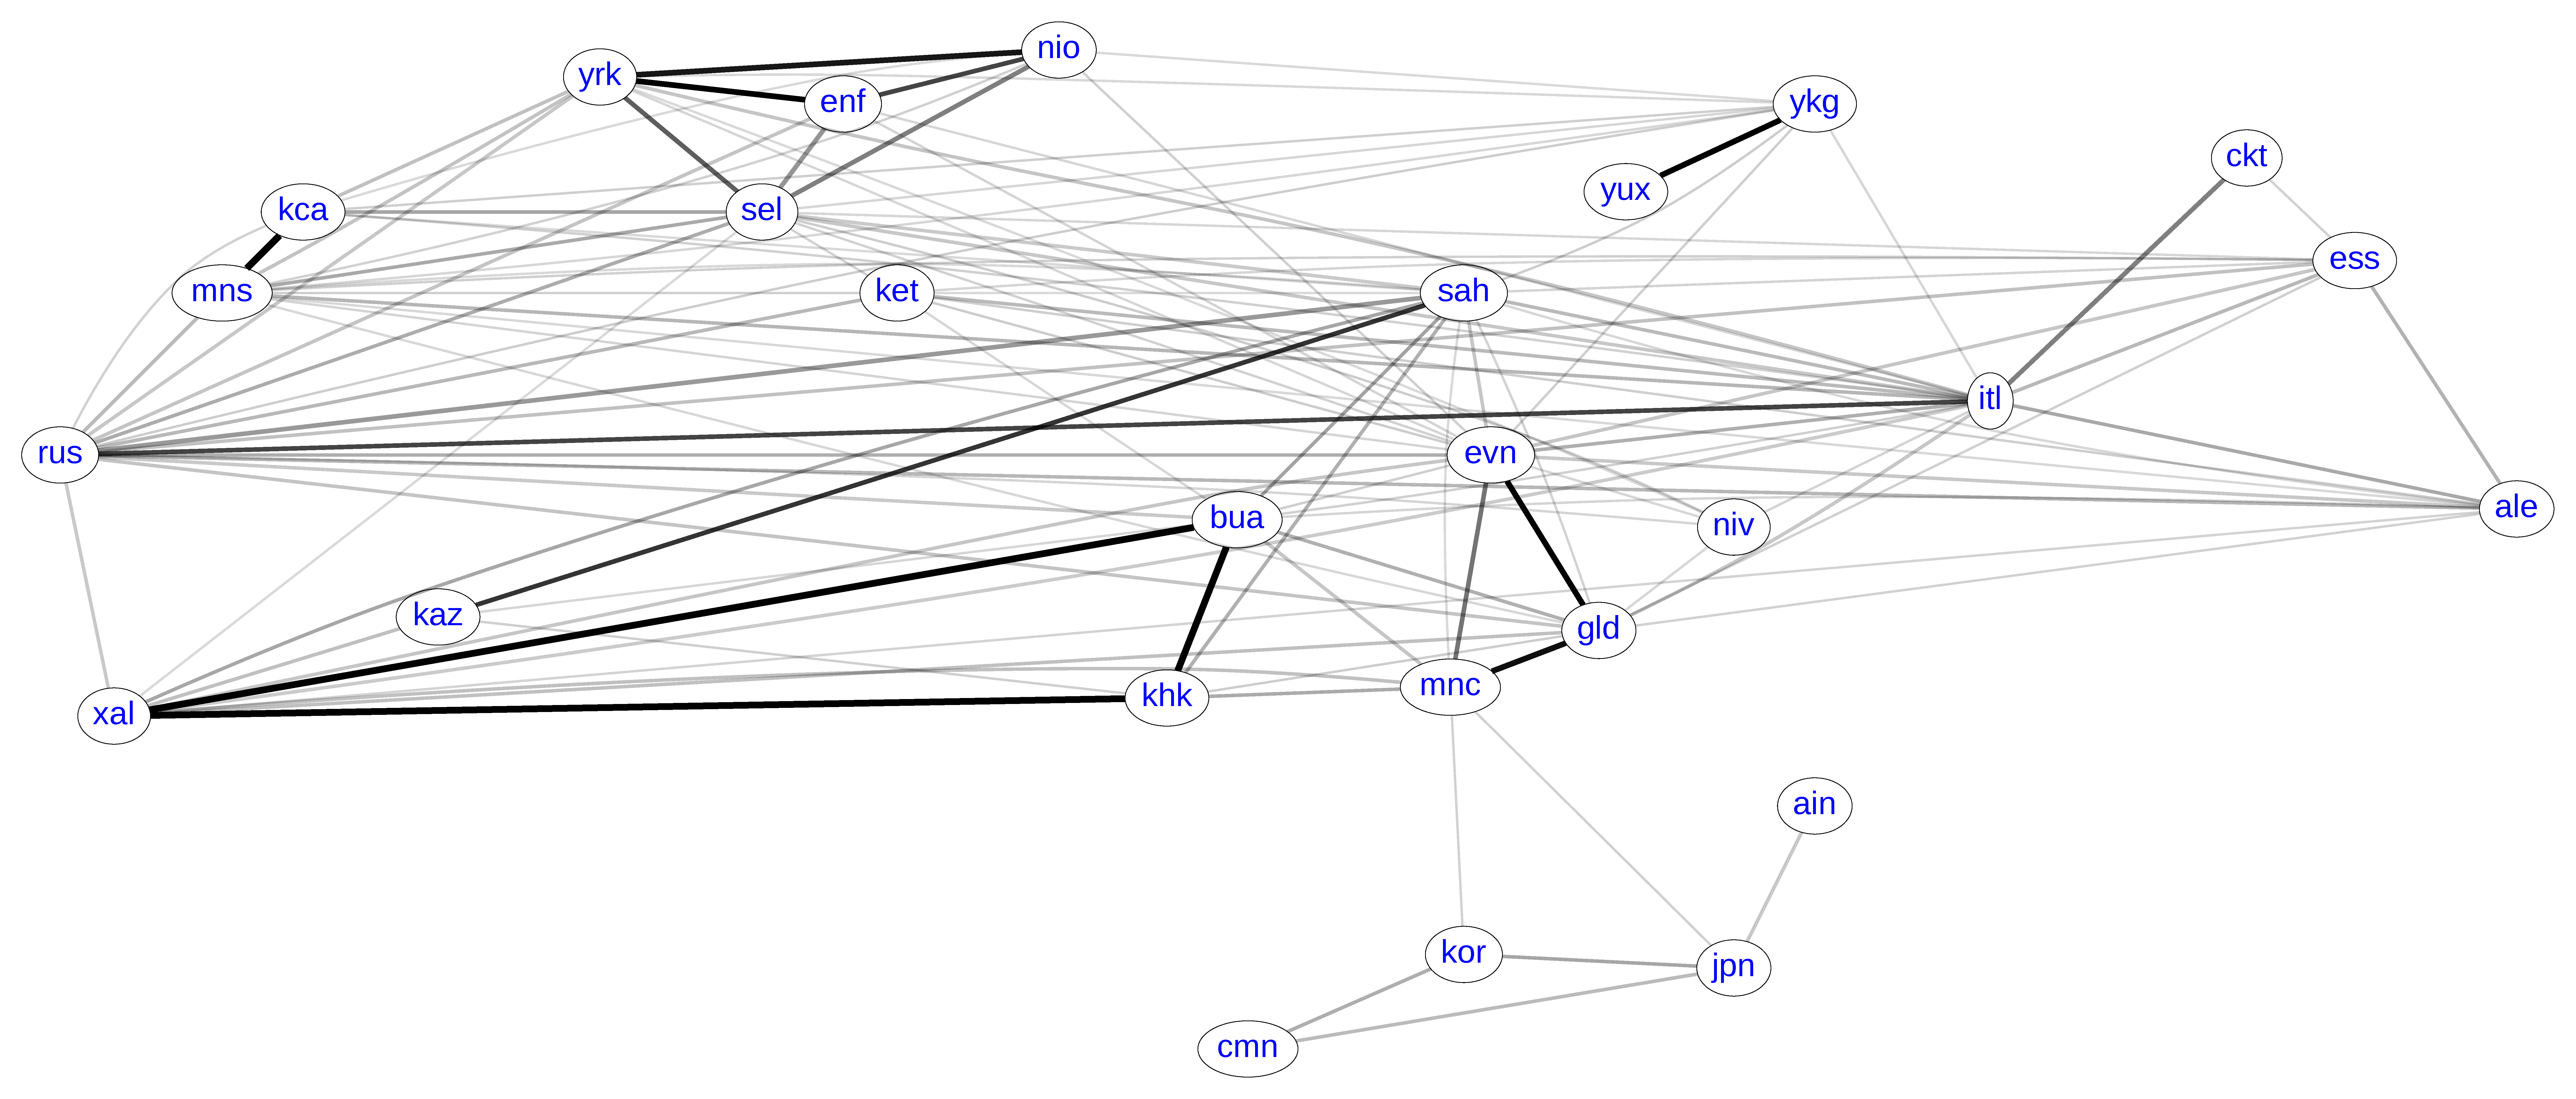
\includegraphics[width=\textwidth]{figures/cognacy-strength-siberia.pdf}
\caption{Visualization of inferred cognate overlap in the Siberian data}
\label{siberia-cognacy}
\end{sidewaysfigure}

\figref{siberia-goldstandard-phylo} visualizes the gold standard network arising from the previous discussion. The star shape of arrows from \ili{Russian} into almost all the languages of Siberia show that unlike in the previous two case studies, we now only have one major cause of lexical overlap between the many small families and isolates. The challenge in this case study is the correct detection of the many isolates. For reasons which will become clear in the next chapter, the directionality of influence between an isolate and a member of a different family is difficult to detect for causal inference. The directionality of contacts between isolates has always been a problem for historical linguists, and we cannot expect the less refined automated methods to solve it.

\begin{sidewaysfigure}

\includegraphics[width=\textwidth]{figures/goldstandard-phylo-siberia.pdf}
\caption{Gold standard for phylogenetic flow on Siberian data}
\label{siberia-goldstandard-phylo}
\end{sidewaysfigure}

\subsection{Case study 4: A visit to the Caucasus}
The Caucasus is by far the linguistically most complex region covered by the NorthEuraLex database. In addition to three indigenous language families, many \ili{Turkic languages}, several branches of Indo-European\il{Indo-European languages} (Iranian\il{Iranian languages}, \ili {Armenian}, and Slavic\il{Slavic languages}), and even a Mongolic language (\ili{Kalmyk}) exist in the region. The Caucasus has been famous for its high density of widely divergent languages since antiquity, receiving the very fitting epithet \textit{\v{g}abal al-alsun} `mountain of tongues' by the Arab geographer al-Mas\textquoteleft udi in the 10th century.

Starting out with the indigenous families, the \textit{Abkhazo-Adyghean} or \textit{Northwest Caucasian} languages\il{Northwest Caucasian languages} (\textit{abk}, \textit{ady}) are a small group of four living languages, which fall into the two primary branches Abkhaz-Abaza\il{Abkhaz-Abaza languages}, consisting of \ili{Abkhaz} (\textit{abk}) and closely related \ili{Abaza}, and the Circassian\il{Circassian languages} dialect continuum, with the literary languages \ili{Adyghe} (\textit{ady}) in the west, and \ili{Kabardian} in the east. Both branches are only represented by a single language in the current version of NorthEuraLex, such that Abkhaz-Abaza will be synonymous with \textit{abk}, and Circassian with \textit{ady}. The Northwest Caucasian languages are typological outliers in Europe, with their predominantly ergative case alignment, phoneme inventories which are very rich in consonants but with minimal numbers of vowels, and, perhaps most interestingly, a very complex verbal morphology where
verbs agree with up to three arguments, instead of just the subject, as is the case in typical European languages. According to \cite{hewitt2004}, both languages in our sample have borrowed some words from \ili{Turkic languages}. The dominant influence, however, occurred after the \ili{Russian} conquest of the Caucasus (\textit{rus} \arrowLA \textit{abk, ady}). In addition, Abkhaz has come under significant pressure by \ili{Georgian} (\textit{kat} \arrowLA \textit{abk}) as the state language of the Georgian SSR. This pressure has subsided since independent Georgia lost control of Abkhazia after a civil war in 1992, which is now a de-facto independent state without international recognition.

The \textit{Nakho-Daghestanian}\il{Nakho-Daghestanian languages} or \textit{Northeast Caucasian}\il{Northeast Caucasian languages} languages (\textit{che}, \textit{ava}, \textit{lez}, \textit{dar}, \textit{lak}, \textit{ddo}) are spoken mainly in the Russian republics of Daghestan, Chechnya, and Ingushetia. The family is well-known for featuring the world's most extensive case systems, and the largest noun class systems after the \ili{Bantu languages}. NorthEuraLex contains a sample of six Northeast Caucasian languages, falling short of the goal of having one representative on each branch, but containing all the literary languages for which large dictionaries are readily available. The about 40 languages of the family can be grouped into seven uncontested branches, but the structure of the larger subunits is still subject to debate, much as in the case of Uralic. Traditionally, the family was split into a Nakh\il{Nakh languages} branch containing the closely related literary languages \ili{Chechen} (\textit{che})
and \ili{Ingush}, and a Daghestanian\il{Daghestanian languages} branch comprising all the other branches. Among the languages of Daghestan, a general consensus seems to be that the \ili{Avar-Andic languages}, to which the lingua franca \ili{Avar} (\textit{ava}) belongs, are more closely related to the \ili{Tsezic languages}, which are represented in NorthEuraLex by \ili{Tsez} (\textit{ddo}), than to the other branches of Nakho-Daghestanian. The other Daghestanian branches are the \ili{Dargin languages} represented by Literary \ili{Dargwa} (\textit{dar}), the \ili{Lezgic languages} represented by \ili{Lezgian} (\textit{lez}), and the isolates \ili{Lak} (\textit{lak}) and \ili{Khinalugh}, the latter of which is not part of NorthEuraLex. While Tsez and many other small Daghestanian languages are endangered, the five large literary languages in our sample can be considered sociolinguistically stable, even though bilingualism with \ili{Russian} is by now almost universal \citep{hewitt2004}. During their history,
all Northeast Caucasian languages have borrowed substantial amounts of lexical material from \ili{Persian}, Oghuz Turkic\il{Oghuz Turkic languages}, and \ili{Russian}, the languages of neighboring empires vying for control of the Caucasus (\textit{rus}, \textit{pes}, \textit{azj} \arrowLA \textit{che}, \textit{ava}, \textit{lez}, \textit{dar}, \textit{lak}, \textit{ddo}). Influence from smaller \ili{Turkic languages} such as \ili{Kumyk} and \ili{Nogai} has also existed for centuries. Due to the close similarity of these languages with \ili{Azeri} in their basic vocabulary, most of these influences can be subsumed under the incoming lexical flow from Azeri, although some signal will be lost due to the absence of these Turkic languages of the Caucasus in our sample. Finally, Avar has influenced the other languages of Daghestan due to its role as a lingua franca of the region (\textit{ava} \arrowOA \textit{lez}, \textit{dar}, \textit{lak}, \textit{ddo}).

The third language family native to the Caucasus, \textit{Kartvelian}\il{Kartvelian languages} or South Caucasian\il{South Caucasian languages}, consists of the \ili{Georgian} language (\textit{kat}), the only indigenous Caucasian language with an ancient literary tradition, three closely related minority languages which are often treated as variants of Georgian, and more distantly related \ili{Svan}, all of which are not yet represented in NorthEuraLex. Like most languages in the region, Georgian was influenced intensively by \ili{Persian} (\textit{pes} \arrowLA \textit{kat}) and \ili{Turkic languages} (\textit{azj} \arrowLA \textit{kat}). Russian influence on basic vocabulary is rather limited in comparison, because Georgian was influenced much more from its southern neighbors when its statehood and cultural identity was formed in the Middle Ages. \cite{khalilov1993} systematically describes the language contacts between Georgian and neighboring \ili{Northeast Caucasian languages}. The main conclusion
is that the borrowings from \ili{Daghestanian languages} into eastern dialects of Georgian do not appear in the Georgian literary language, and should therefore not be visible in our dataset. In the reverse direction, intensive borrowing took place in the nominal domain, where also many Iranian\il{Iranian languages} loans were transmitted into Daghestan via Georgian. The only two Daghestanian languages in the sample whose lexicon was significantly influenced by Georgian are \ili{Avar} (\textit{kat} \arrowLA \textit{ava}) and \ili{Tsez} (\textit{kat} \arrowLA \textit{ddo}), the immediate eastern neighbors of Georgian. Contacts with \ili{Nakh languages} such as \ili{Chechen} did exist, but did not leave substantial traces in the basic vocabulary of either Georgian or Chechen.

The \textit{Iranian}\il{Iranian languages} branch of Indo-European (\textit{kur}, \textit{pes}, \textit{oss}, \textit{pbu}) has been one of the decisive factors which shaped the linguistic landscape of the Caucasus. The Iranian languages are classified into the two subgroups Western Iranian\il{Western Iranian languages} and Eastern Iranian\il{Eastern Iranian languages}, each of which can be separated into a northern and a southern branch. NorthEuraLex contains the dominant language of each of the four groups.

\ili{Ossetian} (\textit{oss}), one of two extant Northeast Iranian languages (the other being \ili{Yaghnobi} in Tajikistan), is taken to be a direct descendant of the \ili{Scytho-Sarmatian languages} spoken by Iranian peoples all over the Central Asian steppes since the 8th century BC. Modern Ossetian is split into two varieties, the larger of which, Iron, is spoken by about 570,000 speakers in both North and South Ossetia, and is the variant represented in NorthEuraLex. According to \cite{thordarson2009}, evidence from placenames in the Northwest Caucasus suggests that the Ossetes once lived further to the west, where Turkic\il{Turkic languages} and \ili{Circassian languages} are spoken today, and that a Nakh language related to \ili{Ingush} was spoken in North Ossetia. These interactions have left their traces in the lexicon, and Iron Ossetic contains layers of loanwords from Circassian (\textit{ady} \arrowLA \textit{oss}), Nakh (\textit{che} \arrowLA \textit{oss}), and Turkic languages (\textit{Turkic} \arrowLA \textit{oss}).

\ili{Pashto} (\textit{pbu}), the only important Southeast Iranian language, is spoken by about 50 million people in Southern Afghanistan and Northern Pakistan. Modern Pashto is not of immediate relevance to the Caucasus, but an important second datapoint in addition to Ossetian for reconstructing the cognate sets present in Eastern Iranian, which can be expected to lead to a clearer picture. The two largest lexical influences on Pashto are \ili{Persian} and \ili{Hindi}-\ili{Urdu} (\textit{pes}, \textit{hin} \arrowOA \textit{pbu}), the languages of neighboring states with a lot of cultural influence on the mountains inhabited by Pashtun tribes. Some additional religious and scientific terminology was borrowed directly from \ili{Arabic} as well (\textit{arb} \arrowLA \textit{pbu}).

Modern \ili{Persian} (\textit{pes}), the only major Southwestern Iranian language, is spoken under different names in Iran (Farsi), Northern Afghanistan (Dari), and Tajikistan (Tajik). As the state language of the Persian empire as well as modern Iran, and the predominant language of literature and science in the region, Persian has been a major source of lexical material for all neighboring languages, including \ili{Turkish} and \ili{Hindi}. In these contacts, Persian also served as a transmitter language for much religious and scientific vocabulary which the Persians borrowed from the Arabs together with Islam (\textit{arb} \arrowLA \textit{pes}). Loans from Turkic\il{Turkic languages} and \ili{Mongolic languages} into Persian do exist, but they are mostly confined to the military and the administration.

By far the most important Northwestern Iranian language is \ili{Kurdish}, with an estimated 30 million speakers. Of the different variants of Kurdish, NorthEuraLex samples the \ili{Kurmanji} language (\textit{kmr}) by a dialect spoken in Turkey near the Syrian border, i.e.\ in the center of the Kurdish-speaking lands. During its history, all variants of Kurdish have borrowed substantially from their \ili{Arabic}-speaking southern neighbors (\textit{arb} \arrowLA \textit{kmr}), and to a much lesser degree from the Armenians\il{Armenian} to the north. Also, as any state language on a minority language, Turkish has left lexical traces in the NorthEuraLex variant Kurmanji (\textit{tur \arrowLA kmr}), whereas an Iranian variant would have displayed a strong recent influence from Persian.

\ili{Armenian} (\textit{hye}), the oldest Indo-European language of the Caucasus, forms a separate branch of the family, with possible deep affinities to \ili{Greek}. In addition to a layer of very early loans from Kartvelian\il{Kartvelian languages} (\textit{kat} \arrowLA \textit{hye}) and some borrowings from \ili{Northeast Caucasian languages}, Armenian has been under pervasive influence from various \ili{Iranian languages} throughout its history, to the point that it was long itself considered an Iranian language. \cite{bailey1987} discusses the different layers of Iranian loanwords which have been the subject of more than a century of research, and are so rich that their analysis contributed to a better understanding of the development of Middle Iranian. Since some of the loans go back as far as the Old Iranian period, it makes sense to include \textit{Iranian} \arrowOA \textit{hye} in the gold standard in order to model the ancient connections. As later cultural vocabulary overwhelmingly came from
variants of \ili{Persian}, I additionally include a link \textit{pes} \arrowOA \textit{hye}.

Turkic presence in the Caucasus goes back to the arrival of Oghur tribes in the 7th century, who formed the Bulgar and Khazar khanates in the Pontic and Caspic steppes. Too little is known about these languages to decide whether Turkic loans in the North Caucasus can be traced back to this time, or whether they occured during the time of the Pecheneg khanates, who occupied the same area in the 10th and 11th centuries. The influence of their \ili{Pecheneg} language, which belongs to the Oghuz\il{Oghuz Turkic languages} branch of Turkic, is approximated in the gold standard by \ili{Azeri} (\textit{azj}). The next Turkic-speaking steppe state, the Cuman-Kipchak confederation of the 12th century, brought the Kipchak languages\il{Kipchak Turkic languages} spoken by today's Turkic inhabitants of the North Caucasus, such as \ili{Karachay-Balkar} in the Northwest Caucasus, the \ili{Nogai} language in the center, and \ili{Kumyk} in Northern Daghestan. These languages especially influenced the \ili{Circassian
languages}, \ili{Chechen}, and the Northern Daghestanian languages \ili{Dargwa} and \ili{Avar} (\textit{Kipchak} \arrowLA \textit{ady, che, dar, ava}). All of these contacts will be represented by means of the only Kipchak language, \ili{Kazakh}, in the language sample for this case study. As an additional datapoint, I also add \ili{Uzbek} (\textit{uzn}) to the dataset, which does not appear to have any relevant contacts into the Caucasus beyond the Common Turkic layer represented by the other three languages. On the south side of the Caucasus, \ili{Ottoman Turkish} borrowed extensively from Arabic (\textit{arb} \arrowLA \textit{tur}), the language of the southern half of the Ottoman Empire, and in turn influenced the \ili{Arabic} dialects in Syria and Iraq. Like most languages of the region, Turkish, Azeri, and Uzbek have many loans from \ili{Persian} (\textit{pes} \arrowLA \textit{tur, azj, uzn}).

Eastern influences on \ili{Russian} (\textit{rus}) and the lexical sources for the Mongolic language Kalmyk (\textit{xal}) were already discussed in the previous section. The \textit{Semitic} languages\il{Semitic languages} represented in NorthEuraLex, \ili{Arabic} (\textit{arb}) and \ili{Hebrew} (\textit{heb}), were not strongly influenced by any languages from the north. Still, Arabic needs to be included as an important source of religious and scientific vocabulary for the entire Islamic world. Hebrew, the most important Northwest Semitic language which shares hundreds of cognates in basic vocabulary with Arabic, did not interact much with any languages of the Caucasus area, but still seemed worthwhile to include as a test case for the absence of lexical flow.

The cognate overlaps visualized in \figref{caucasus-cognacy} show that the lexical flow inference problem on this set is again different in structure from the other three example scenarios. This time, there are multiple poles causing lexical overlaps across much of the region, as Arabic, Iranian, Russian, and Turkic material are all very widespread. A large part of the lexical flow inference task consists in answering the question whether e.g.\ some of the overlaps with Arabic can be explained away by Persian or Turkic as intermediates.

\begin{figure}
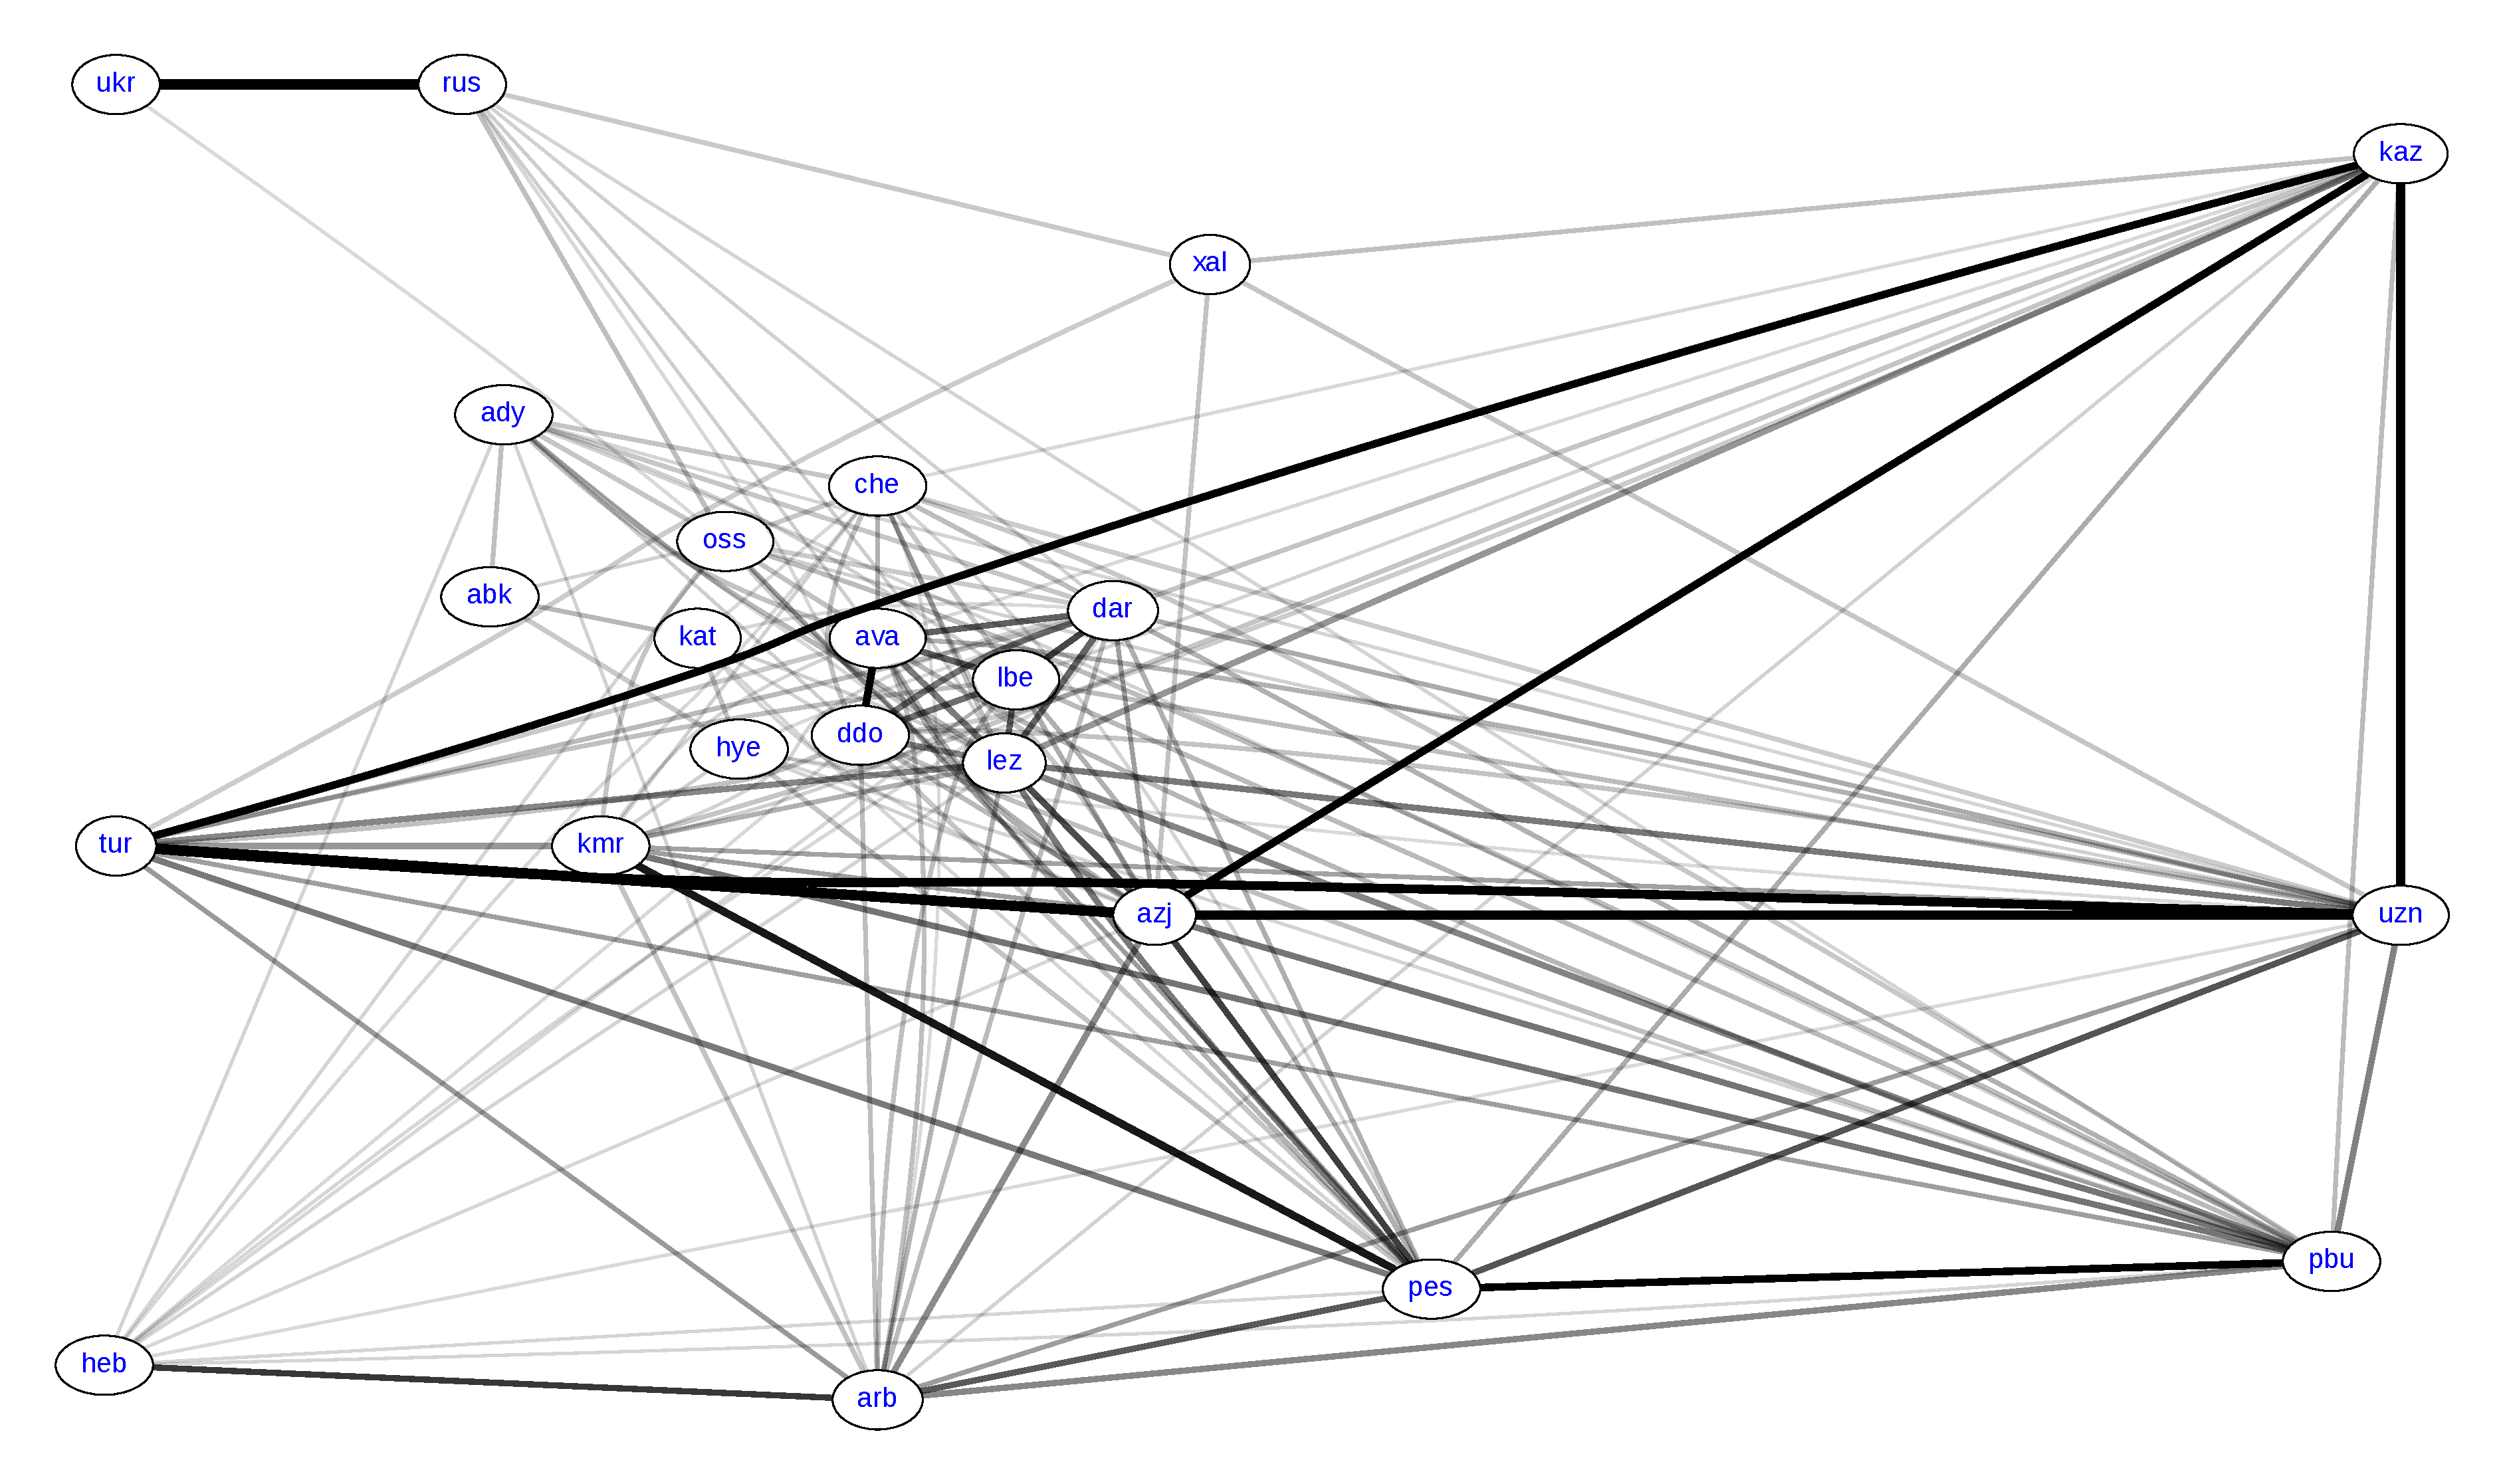
\includegraphics[width=\textwidth]{figures/cognacy-strength-caucasus.pdf}
\caption{Visualization of inferred cognate overlap in the Caucasian data}
\label{caucasus-cognacy}
\end{figure}

\figref{caucasus-goldstandard-phylo} shows the gold standard for phylogenetic inference. It is easy to glimpse that this scenario is by far the most challenging to get right, due to the very complex interactions among the native languages of the Caucasus, which are additionally influenced by the four major external sources of lexical material mentioned above.

\begin{figure}
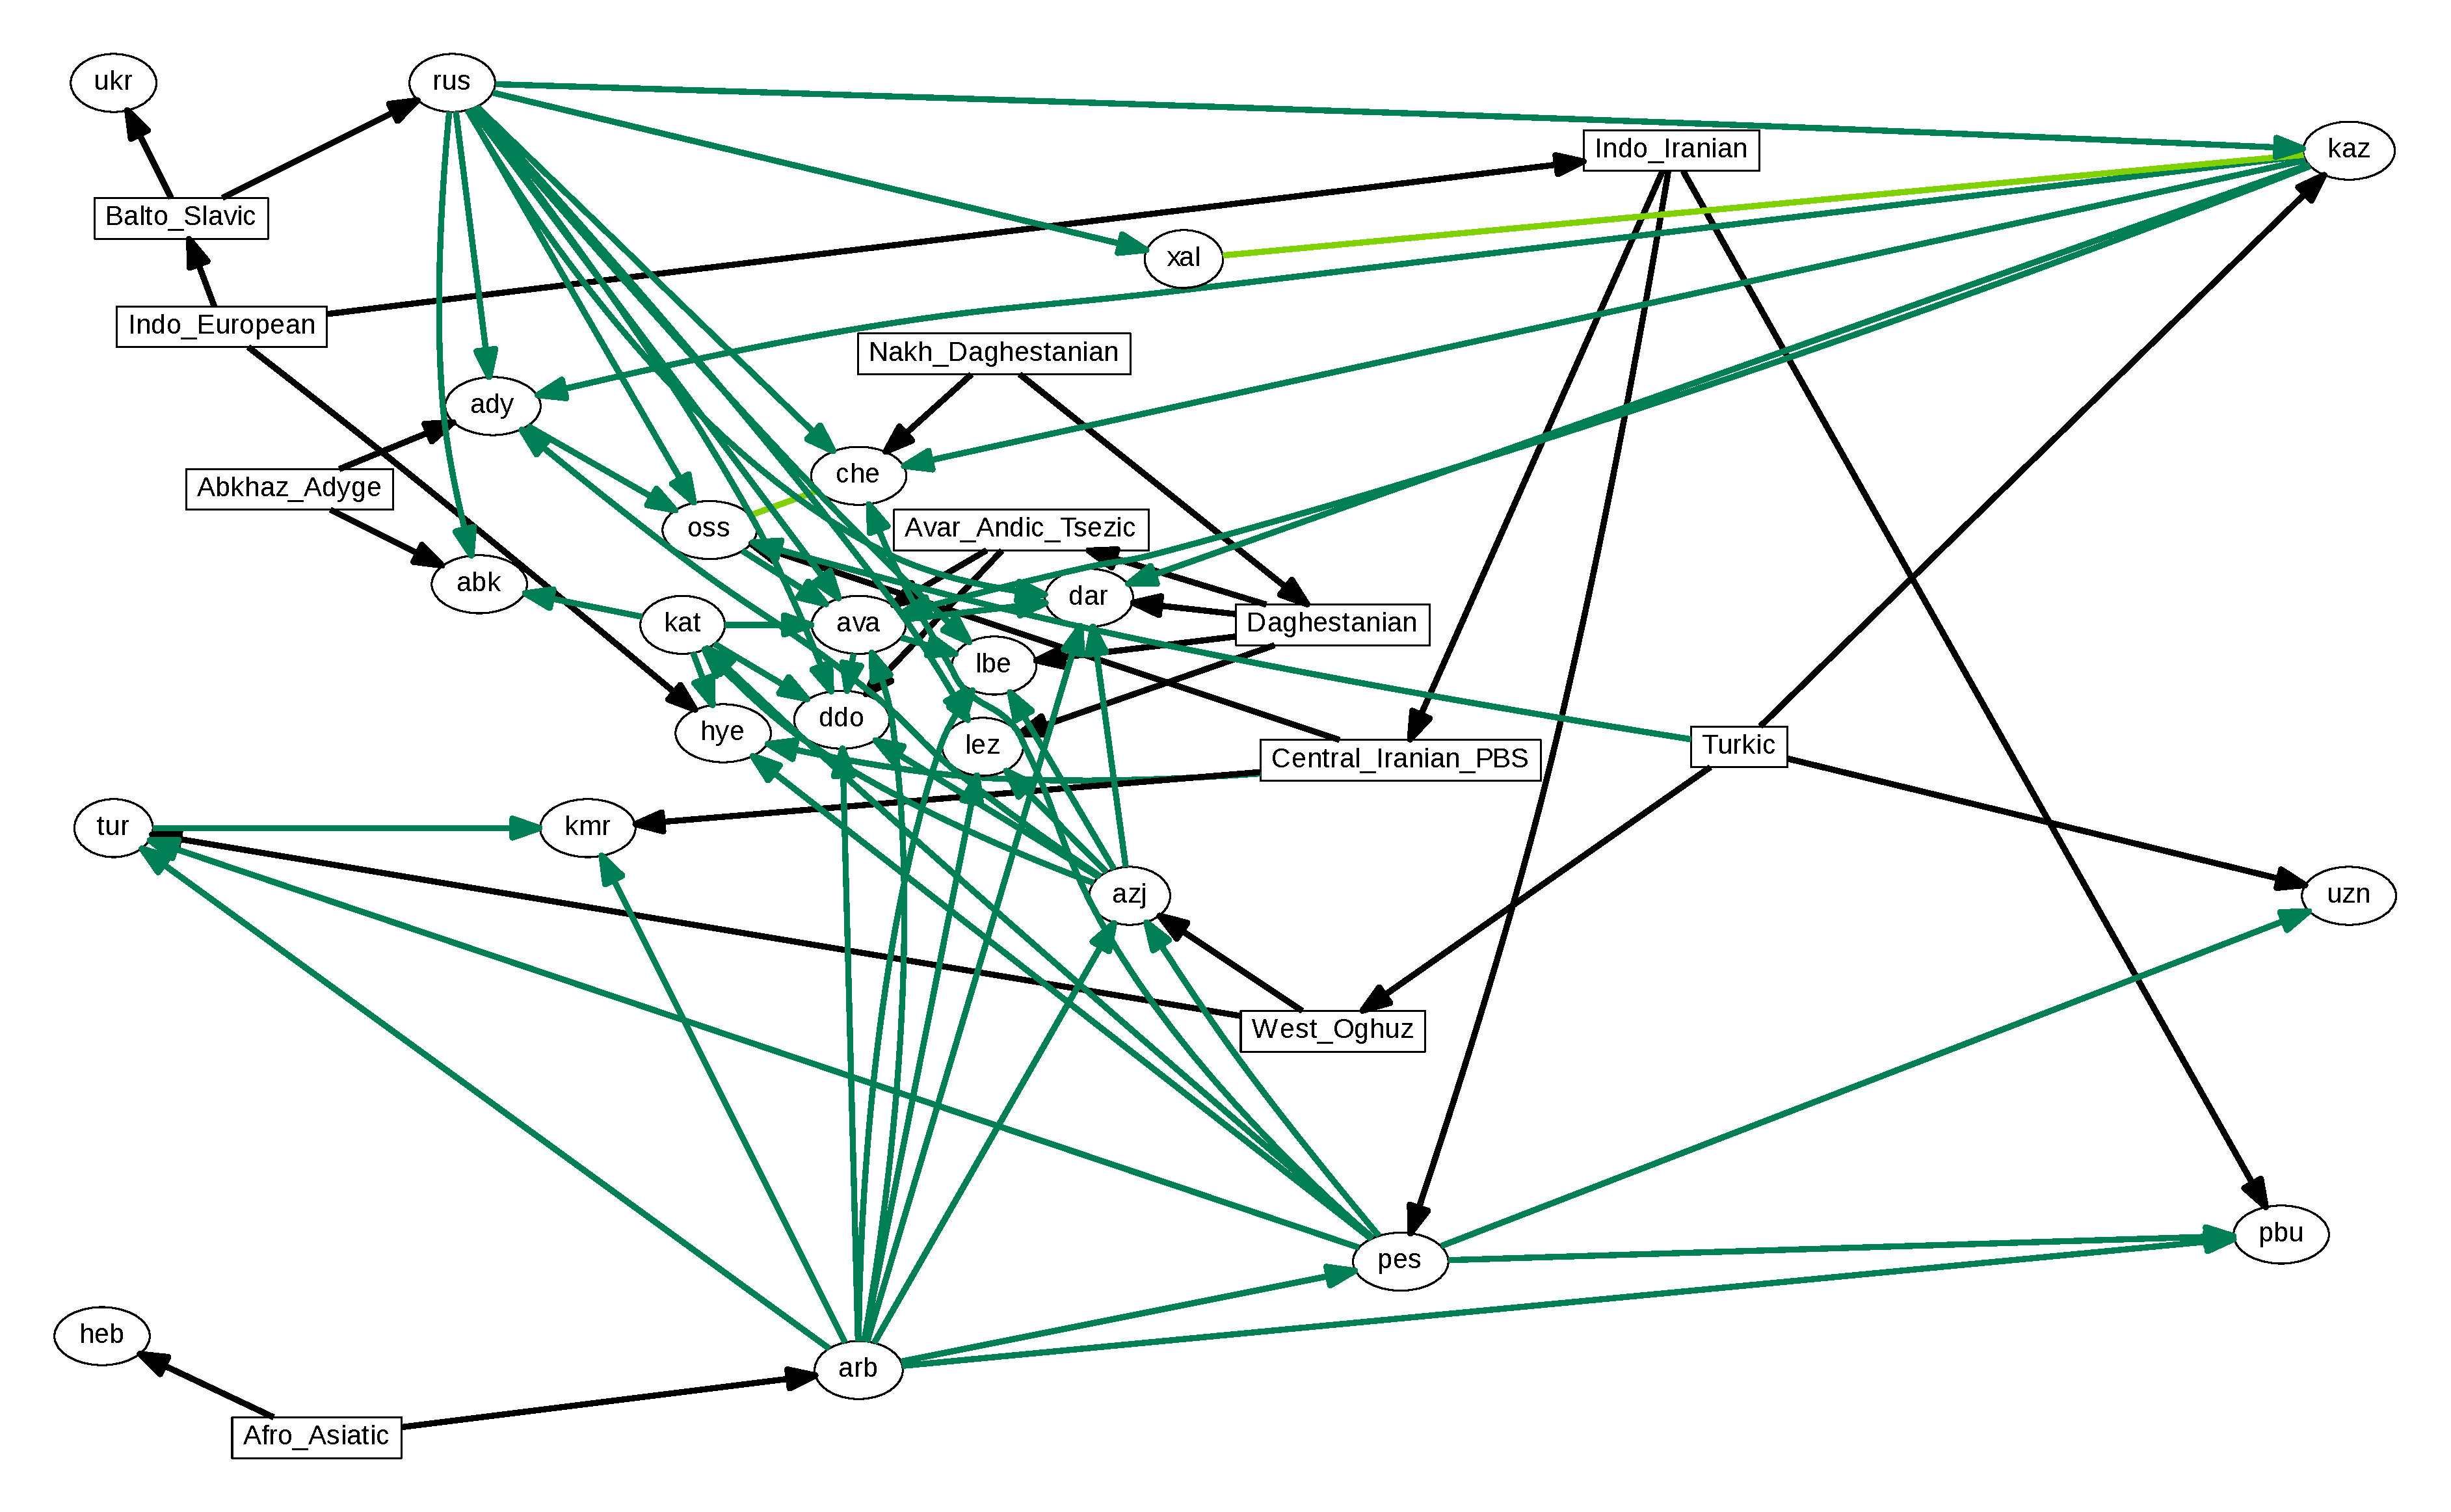
\includegraphics[width=\textwidth]{figures/goldstandard-phylo-caucasus.pdf}
\caption{Gold standard for phylogenetic flow on Caucasian data}
\label{caucasus-goldstandard-phylo}
\end{figure}

After presenting the four test scenarios derived from true linguistic histories, we now turn to the way in which any number of additional test scenarios can be synthesized in order to gain a better picture of the comparative performance of different approaches to lexical flow inference.
